% -------------------------
% Document class
% -------------------------
\documentclass[aspectratio=169]{beamer}

% -------------------------
% Theme & macros
% -------------------------
% -------------------------
% Packages
% -------------------------
\usepackage[T1]{fontenc}
\usepackage{lmodern}
\usepackage{geometry}
\usepackage{xcolor}
\usepackage{graphicx}
\usepackage{tikz}

% Do not set paperwidth/paperheight here.
% Keep original size from:
% \documentclass[aspectratio=169]{beamer}

% -------------------------
% Theme
% -------------------------
\usetheme{Madrid}
% \usecolortheme{default}

% -------------------------
% Colors
% -------------------------
\definecolor{RLBlue}{RGB}{58,53,183}
\definecolor{RLWhite}{RGB}{255,255,255}
\definecolor{RLGreen}{RGB}{95,160,164}
\definecolor{RLOrange}{RGB}{244,189,112}
\definecolor{RLGray}{RGB}{250,249,246}

% Title page colors
\setbeamercolor{title}{fg=RLWhite}
\setbeamercolor{subtitle}{fg=RLWhite}
\setbeamercolor{author}{fg=RLWhite}
\setbeamercolor{institute}{fg=RLWhite}
\setbeamercolor{date}{fg=RLWhite}

% -------------------------
% Main Beamer colors
% -------------------------
\setbeamercolor{structure}{fg=RLBlue}
\setbeamercolor{frametitle}{fg=RLWhite,bg=RLBlue}
\setbeamercolor{block title}{fg=RLWhite,bg=RLGreen}
\setbeamercolor{block body}{bg=RLGray}
\setbeamercolor{alerted text}{fg=RLOrange}


\definecolor{ShortsPanel}{HTML}{2F2A9A}
\definecolor{ShortsText}{HTML}{F5F7FA}
\definecolor{ShortsMuted}{HTML}{C7CDD6}
\definecolor{ShortsAccent}{HTML}{8EDFFF}
\definecolor{ShortsWarm}{HTML}{FFD58A}

% -------------------------
% Footer colors
% -------------------------
\definecolor{FooterLeft}{HTML}{1F6AA5}
\definecolor{FooterCenter}{HTML}{5A57D6}
\definecolor{FooterRight}{HTML}{2D8A57}
\definecolor{FooterContacts}{HTML}{4A3FB8}
\definecolor{FooterContactA}{HTML}{F4F7FB}
\definecolor{FooterContactB}{HTML}{EAF4FF}
\definecolor{FooterContactC}{HTML}{E9FBF8}
\definecolor{FooterContactD}{HTML}{F1ECFF}
\definecolor{FooterContactE}{HTML}{E8F1FF}
\definecolor{FooterIconA}{HTML}{EAF4FF}
\definecolor{FooterIconB}{HTML}{EAF4FF}
\definecolor{FooterIconC}{HTML}{E9FBF8}
\definecolor{FooterIconD}{HTML}{F1ECFF}
\definecolor{FooterIconE}{HTML}{E8F1FF}
\definecolor{FooterIconDark}{HTML}{1F2450}
\definecolor{FooterIconYouTube}{HTML}{E11D48}
\definecolor{FooterIconPhone}{HTML}{0F766E}
\setbeamercolor{author in head/foot}{fg=ShortsText,bg=FooterLeft}
\setbeamercolor{title in head/foot}{fg=ShortsText,bg=FooterCenter}
\setbeamercolor{date in head/foot}{fg=ShortsText,bg=FooterRight}
\setbeamercolor{footer contacts}{fg=ShortsText,bg=FooterContacts}

\setbeamertemplate{navigation symbols}{}

% -------------------------
% Logo placement
% -------------------------
\newcommand{\RLCompanyLogo}{images/company-logo.png}

\addtobeamertemplate{title page}{}{%
  \begin{tikzpicture}[remember picture,overlay]
    \node[anchor=center,yshift=-0.4in]
      at (current page.center)
      {\includegraphics[height=1.15in]{\RLCompanyLogo}};
  \end{tikzpicture}%
}

\makeatletter
\setbeamertemplate{frametitle}{%
  \nointerlineskip%
  \begin{beamercolorbox}[
    wd=\paperwidth,
    ht=0.52in,
    dp=0.08in,
    sep=0pt
  ]{frametitle}%
    \vbox to 0.52in{%
      \vfil%
      \hbox to \paperwidth{%
        \hspace*{0.18in}%
        \begin{minipage}[t]{0.76\paperwidth}%
          {\usebeamerfont{frametitle}\insertframetitle\par}%
          \ifx\insertframesubtitle\@empty\else%
            \vspace{-0.1em}%
            {\usebeamerfont{framesubtitle}\insertframesubtitle\par}%
          \fi%
        \end{minipage}%
        \hfill%
        \raisebox{-0.03in}{\includegraphics[height=0.30in]{\RLCompanyLogo}}%
        \hspace*{0.18in}%
      }%
      \vfil%
    }%
  \end{beamercolorbox}%
}
\makeatother

% -------------------------
% Contact values
% -------------------------
\newcommand{\RLFooterServiceTitle}{Contact us for AI/IT solutions, projects, consulting, and hardware}
\newcommand{\RLFooterTelegram}{@tqqt\_llc}
\newcommand{\RLFooterEmail}{musulmon.lolayev.94@gmail.com}
\newcommand{\RLFooterInstagram}{@tqqt\_llc}
\newcommand{\RLFooterLinkedIn}{linkedin.com/in/tqqt\_llc}
\newcommand{\RLFooterYouTube}{youtube.com/@tqqt\_llc}
\newcommand{\RLFooterPhone}{+998900667801}
\newcommand{\RLFooterWebsite}{tqqt.uz}

% -------------------------
% Icons
% -------------------------
\newcommand{\TelegramIcon}{%
  \tikz[baseline=-0.45ex,x=1pt,y=1pt]{%
    \path[use as bounding box] (-4,-4) rectangle (4,4);
    \fill[white] (0,0) circle (3.6);
    \fill[FooterIconDark]
      (-2.8,0.1) -- (2.9,2.4) -- (1.1,-2.8) --
      (-0.2,-0.7) -- (-1.8,-1.8) -- cycle;
  }%
}

\newcommand{\EmailIcon}{%
  \tikz[baseline=-0.45ex,x=1pt,y=1pt]{%
    \path[use as bounding box] (-4,-4) rectangle (4,4);
    \fill[white] (0,0) circle (3.6);
    \draw[FooterIconDark,line width=0.8pt,rounded corners=0.8pt]
      (-2.6,-1.8) rectangle (2.6,1.8);
    \draw[FooterIconDark,line width=0.8pt]
      (-2.6,1.8) -- (0,-0.4) -- (2.6,1.8);
    \draw[FooterIconDark,line width=0.7pt]
      (-2.6,-1.8) -- (-0.8,0.3);
    \draw[FooterIconDark,line width=0.7pt]
      (2.6,-1.8) -- (0.8,0.3);
  }%
}

\newcommand{\InstagramIcon}{%
  \tikz[baseline=-0.45ex,x=1pt,y=1pt]{%
    \path[use as bounding box] (-4,-4) rectangle (4,4);
    \fill[white] (0,0) circle (3.6);
    \draw[FooterIconDark,line width=0.8pt,rounded corners=1.2pt]
      (-2.35,-2.35) rectangle (2.35,2.35);
    \draw[FooterIconDark,line width=0.75pt] (0,0) circle (1.15);
    \fill[FooterIconDark] (1.75,1.75) circle (0.35);
  }%
}

\newcommand{\LinkedInIcon}{%
  \tikz[baseline=-0.45ex,x=1pt,y=1pt]{%
    \path[use as bounding box] (-4,-4) rectangle (4,4);
    \fill[white] (0,0) circle (3.6);
    \node[text=FooterIconDark,font=\bfseries\tiny] at (0,-0.15) {in};
  }%
}

\newcommand{\YouTubeIcon}{%
  \tikz[baseline=-0.45ex,x=1pt,y=1pt]{%
    \path[use as bounding box] (-4,-4) rectangle (4,4);
    \fill[white] (0,0) circle (3.6);
    \fill[FooterIconDark,rounded corners=1.0pt] (-2.7,-1.65) rectangle (2.7,1.65);
    \path[fill=white] (1.1,0) -- (-0.9,1.1) -- (-0.9,-1.1) -- cycle;
  }%
}

\newcommand{\PhoneIcon}{%
  \tikz[baseline=-0.45ex,x=1pt,y=1pt]{%
    \path[use as bounding box] (-4,-4) rectangle (4,4);
    \fill[white] (0,0) circle (3.6);
    \draw[FooterIconDark,line width=0.85pt,rounded corners=0.9pt]
      (-1.75,-2.85) rectangle (1.75,2.85);
    \draw[FooterIconDark,line width=0.55pt]
      (-1.05,-1.75) rectangle (1.05,1.65);
    \fill[FooterIconDark] (-0.45,2.25) rectangle (0.45,2.4);
    \fill[FooterIconDark] (0,-2.35) circle (0.28);
  }%
}

\newcommand{\WebsiteIcon}{%
  \tikz[baseline=-0.45ex,x=1pt,y=1pt]{%
    \path[use as bounding box] (-4,-4) rectangle (4,4);
    \fill[white] (0,0) circle (3.6);
    \draw[FooterIconDark,line width=0.75pt] (0,0) circle (2.45);
    \draw[FooterIconDark,line width=0.65pt] (-2.45,0) -- (2.45,0);
    \draw[FooterIconDark,line width=0.65pt] (0,-2.45) -- (0,2.45);
    \draw[FooterIconDark,line width=0.55pt]
      (-2.1,1.75) .. controls (0,0.85) .. (2.1,1.75);
    \draw[FooterIconDark,line width=0.55pt]
      (-2.1,-1.75) .. controls (0,-0.85) .. (2.1,-1.75);
  }%
}

% -------------------------
% Footer: two rows
% -------------------------
\newlength{\RLFooterTopHeight}
\newlength{\RLFooterBottomHeight}
\setlength{\RLFooterTopHeight}{0.13in}
\setlength{\RLFooterBottomHeight}{0.13in}

\setbeamertemplate{footline}{%
  \leavevmode%
  \vbox{%
    % Row 1: title | service title | page number
    \hbox{%
      \begin{beamercolorbox}[
        wd=.22\paperwidth,
        ht=\RLFooterTopHeight,
        dp=0pt,
        sep=0pt
      ]{author in head/foot}%
        \vbox to \RLFooterTopHeight{%
          \vfil
          \hbox to \linewidth{%
            \hspace*{0.10in}%
            {\bfseries\fontsize{6.2}{6.8}\selectfont \inserttitle}%
            \hfil
          }%
          \vfil
        }%
      \end{beamercolorbox}%

      \begin{beamercolorbox}[
        wd=.60\paperwidth,
        ht=\RLFooterTopHeight,
        dp=0pt,
        sep=0pt
      ]{title in head/foot}%
        \vbox to \RLFooterTopHeight{%
          \vfil
          \hbox to \linewidth{%
            \hfil
            {\bfseries\fontsize{6.0}{6.6}\selectfont \RLFooterServiceTitle}%
            \hfil
          }%
          \vfil
        }%
      \end{beamercolorbox}%

      \begin{beamercolorbox}[
        wd=.18\paperwidth,
        ht=\RLFooterTopHeight,
        dp=0pt,
        sep=0pt
      ]{date in head/foot}%
        \vbox to \RLFooterTopHeight{%
          \vfil
          \hbox to \linewidth{%
            \hfil
            {\fontsize{5.8}{6.2}\selectfont \insertframenumber/\inserttotalframenumber}%
            \hspace*{0.08in}%
          }%
          \vfil
        }%
      \end{beamercolorbox}%
    }%

    % Row 2: all contacts
    \hbox{%
      \begin{beamercolorbox}[
        wd=\paperwidth,
        ht=\RLFooterBottomHeight,
        dp=0pt,
        sep=0pt
        ]{footer contacts}%
        \vbox to \RLFooterBottomHeight{%
          \vfil
          \hbox to \linewidth{%
            \hspace*{0.10in}%
            \begin{tabular}{@{}l@{\hspace{0.02in}}l@{\hspace{0.05in}}l@{\hspace{0.02in}}l@{\hspace{0.05in}}l@{\hspace{0.02in}}l@{\hspace{0.05in}}l@{\hspace{0.02in}}l@{\hspace{0.05in}}l@{\hspace{0.02in}}l@{\hspace{0.05in}}l@{\hspace{0.02in}}l@{\hspace{0.05in}}l@{\hspace{0.02in}}l@{}}
              \TelegramIcon & {\color{FooterContactA}\fontsize{3.7}{4.1}\selectfont \RLFooterTelegram}
                & \EmailIcon & {\color{FooterContactB}\fontsize{3.7}{4.1}\selectfont \RLFooterEmail}
                & \InstagramIcon & {\color{FooterContactC}\fontsize{3.7}{4.1}\selectfont \RLFooterInstagram}
                & \LinkedInIcon & {\color{FooterContactD}\fontsize{3.7}{4.1}\selectfont \RLFooterLinkedIn}
                & \YouTubeIcon & {\color{FooterContactE}\fontsize{3.7}{4.1}\selectfont \RLFooterYouTube}
                & \PhoneIcon & {\color{FooterContactB}\fontsize{3.7}{4.1}\selectfont \RLFooterPhone}
                & \WebsiteIcon & {\color{FooterContactC}\fontsize{3.7}{4.1}\selectfont \RLFooterWebsite}
            \end{tabular}%
            \hfil
          }%
          \vfil
        }%
      \end{beamercolorbox}%
    }%
  }%
}

% Packages
\usepackage{amsmath,amssymb}
\usepackage{tikz}
\usepackage{pgfplots}
\usetikzlibrary{positioning}


\pgfplotsset{compat=1.18}

% -------------------------
% RL Teaching Blocks
% -------------------------

\newenvironment{rlintuition}{
  \begin{block}{Intuition}
}{
  \end{block}
}

\newenvironment{rldefinition}{
  \begin{block}{Definition}
}{
  \end{block}
}

\newenvironment{rlpitfall}{
  \begin{alertblock}{Common Pitfall}
}{
  \end{alertblock}
}

\newenvironment{rlquestion}{
  \begin{block}{Think About This}
}{
  \end{block}
}


% -------------------------
% Title info
% -------------------------
\title{Advanced AI}
\subtitle{Module 0: Statistics for Advanced AI}
\author{Musulmon Lolaev}
\institute{TQQT LLC}
\date{\today}

\newif\iflectureonly
\newif\ifshowpauses
\showpausestrue

% Set \showpausesfalse to build a static version with all overlays shown at once.
\AtBeginDocument{%
  \let\beamerpause\pause
  \renewcommand{\pause}[1][]{\ifshowpauses\beamerpause[#1]\fi}
}

\begin{document}

\begin{frame}
\titlepage
\end{frame}

% \section{Module 0: Statistics for Advanced AI}

\begin{frame}{Why Statistics Before Machine Learning}
\begin{itemize}
  \item Every ML model is trained on a \textbf{sample} and evaluated by \textbf{estimating} how well it will generalize.
  \pause
  \item Loss functions (cross-entropy, MSE) are maximum-likelihood objectives in disguise --- Lecture 5.
  \pause
  \item Bayes' theorem underlies methods from Naive Bayes to diffusion models --- Lecture 2.
  \pause
  \item This module builds the probability and estimation vocabulary that Modules 1--3 assume.
\end{itemize}
\end{frame}

\begin{frame}{Reading Resources}
\begin{itemize}
  \item Primary reference for Module 0, Lectures 1--5: Illowsky \& Dean, \textit{Introductory Statistics 2e} (OpenStax), free at \url{https://openstax.org/details/books/introductory-statistics-2e}.
  \pause
  \item We omit topics not critical for AI: chi-square tests, two-sample $t$-tests, ANOVA, and study-design methodology.
  \pause
  \item Hypothesis testing is deferred to Lecture 10 (Statistical Model Evaluation), its most relevant context for this course.
\end{itemize}
\end{frame}


% \section{Lecture 1, Part 0: Data \& Descriptive Statistics}

\begin{frame}
\vfill
\centering
{\color{RLBlue}\large Lecture 1}

\vspace{0.3em}
{\color{RLBlue}\Large\bfseries Part 0}

\vspace{0.6em}
{\Large Data \& Descriptive Statistics}
\vfill
\end{frame}

\begin{frame}{Learning Goals}
\begin{itemize}
  \item Distinguish data types (categorical vs. numerical, discrete vs. continuous) and read frequency distributions, histograms, and box plots.
  \pause
  \item Compute and interpret measures of center (mean, median, mode) and spread (variance, standard deviation, IQR) -- and explain \emph{why} each one is needed, not just how to compute it.
  \pause
  \item Recognize when a single summary statistic hides the real structure of the data (Anscombe's quartet).
\end{itemize}
\end{frame}

\begin{frame}{Data Types}
\begin{columns}[T]
\column{0.48\textwidth}
\textbf{Categorical (qualitative)}
\begin{itemize}
  \item nominal: no natural order (e.g. eye colour, city of birth)
  \pause
  \item ordinal: ordered, unequal spacing (e.g. rating: low/medium/high)
\end{itemize}

\pause
\column{0.48\textwidth}
\textbf{Numerical (quantitative)}
\begin{itemize}
  \item discrete: countable (e.g. number of children in a family)
  \pause
  \item continuous: measured on a scale (e.g. salary, height)
\end{itemize}
\end{columns}

\pause
\begin{rlintuition}
The data type determines which summary statistics and plots are valid: means and standard deviations only make sense for numerical data; categorical data is summarized with counts and proportions.
\end{rlintuition}
\end{frame}

\begin{frame}{Population, Sample, and Notation}
\begin{rldefinition}
A \textbf{population} is every unit we care about; a \textbf{sample} is the subset we actually measure. A sample of size $n$ is written
\[
x_1, x_2, \dots, x_n,
\qquad
x_i = \text{the } i\text{-th observation}.
\]
\end{rldefinition}
\pause
\begin{itemize}
  \item Our 600 salaries are a \textbf{sample}; the population is every employee in the industry -- too large to measure.
  \pause
  \item \textbf{Example:} five salaries (\$1000s) $\{31, 45, 47, 52, 88\}$ give $n = 5$, $x_1 = 31$, $x_3 = 47$, $x_5 = 88$.
  \pause
  \item \textbf{Summation:} $\sum_{i=1}^{n} x_i = x_1 + x_2 + \dots + x_n$ -- ``add up all $n$ observations''.
  \pause
  \item Latin letters ($\bar{x}$, $s$) are computed \emph{from the sample}; Greek letters ($\mu$, $\sigma$) describe the \emph{population} we cannot see.
\end{itemize}
\end{frame}

% ─── Frequency distributions & histograms ───────────────────────────────────
\begin{frame}{Frequency Distributions \& Histograms}
\begin{columns}[T]
\column{0.50\textwidth}
\small
\begin{itemize}
  \item A \textbf{frequency distribution} counts observations per value or class.
  \pause
  \item A \textbf{histogram} plots those counts as bars -- it shows the \emph{shape} of the data: symmetric, skewed, multi-modal.
  \pause
  \item \textbf{Real event:} 600 employee salaries are \emph{right-skewed} -- most sit between \$40k and \$60k, and a thin tail of high earners reaches \$151k.
  \pause
  \item \textbf{Why:} ``the average salary is \$52k'' hides that half the staff earn below \$48k. The shape shows it; the number alone does not.
\end{itemize}
\column{0.48\textwidth}
\centering
\includegraphics[width=\linewidth]{figures/data_probability/data_probability_salary_histogram.pdf}
\end{columns}
\end{frame}

\begin{frame}{Building a Histogram for a Continuous Variable}
\small
A continuous variable almost never repeats a value, so counting each value separately is useless -- group the values into \textbf{classes} first.
\begin{columns}[T]
\column{0.54\textwidth}
\begin{enumerate}
  \item Range $=\max-\min=\$151\text{k}-\$27\text{k}=\$124\text{k}$.
  \pause
  \item Choose the number of classes $k$ (usually 5--10); here $k=7$.
  \pause
  \item Class width $=\text{range}/k=124/7\approx17.7$, rounded up to a convenient \$20k.
  \pause
  \item Count the observations falling in each class.
  \pause
  \item Draw one bar per class, \textbf{bars touching}: the scale is continuous, so gaps would suggest impossible salaries.
\end{enumerate}
\column{0.44\textwidth}
\centering
\scriptsize
\begin{tabular}{lrr}
\hline
Salary class & Freq. & \% \\
\hline
\$20--40k   & 156 & 26.0 \\
\$40--60k   & 311 & 51.8 \\
\$60--80k   &  89 & 14.8 \\
\$80--100k  &  32 &  5.3 \\
\$100--120k &   7 &  1.2 \\
\$120--140k &   3 &  0.5 \\
\$140--160k &   2 &  0.3 \\
\hline
Total       & 600 &      \\
\hline
\end{tabular}
\end{columns}
\end{frame}

% ─── Measures of center: the mean ───────────────────────────────────────────
\begin{frame}{Why Do We Need the Mean?}
\begin{rldefinition}
For a sample $x_1, \dots, x_n$:
\[
\bar{x} = \frac{1}{n}\sum_{i=1}^{n} x_i
\]
\end{rldefinition}
\pause
\begin{itemize}
  \item \textbf{Why:} decisions need one number, not a spreadsheet of 600 salaries. The mean compresses a whole dataset into one value that can be tracked over time or plugged into a formula (expected cost = mean cost $\times$ volume).
  \pause
  \item \textbf{Numerical example:} the five salaries (\$1000s) $\{31, 45, 47, 52, 88\}$ give $\bar{x} = \frac{31+45+47+52+88}{5} = \frac{263}{5} = 52.6$.
  \pause
  \item \textbf{Everyday means:} a student's grade average, the average monthly temperature in a weather report, a car's average fuel consumption, a player's average points per game -- all the same formula.
\end{itemize}
\end{frame}

\begin{frame}{Why Do We Need the Median?}
\begin{rldefinition}
Sort the sample. The \textbf{median} is the middle value: the $\frac{n+1}{2}$-th observation when $n$ is odd, and the average of the two middle observations when $n$ is even.
\end{rldefinition}
\pause
\begin{itemize}
  \item \textbf{Odd $n$:} $\{31, 45, 47, 52, 88\}$ is sorted and $n = 5$, so the median is the 3rd value, $47$.
  \pause
  \item \textbf{Even $n$:} drop the 88 to get $\{31, 45, 47, 52\}$ with $n = 4$; the median is $\frac{45 + 47}{2} = 46$.
  \pause
  \item For the first set $\bar{x} = 52.6$, which is larger than \emph{four of the five} salaries -- the single \$88k earner pulls it up, while the median stays on the middle person.
  \pause
  \item \textbf{Why:} the median describes a \emph{typical} member of the sample; the mean describes what each would get if the total were shared equally.
\end{itemize}
\end{frame}

\begin{frame}{Real Event: When the Mean Misleads}
\begin{columns}[T]
\column{0.50\textwidth}
\small
\begin{itemize}
  \item Nine people are in a bar, net worth \$20K--\$150K. Mean $\approx$ \$97K, median $\approx$ \$121K -- close together.
  \pause
  \item A billionaire walks in. The \textbf{mean} jumps to \$15{,}000{,}087{,}166 -- nobody in the room is close to that. The \textbf{median} barely moves, to \$122K.
  \pause
  \item \textbf{Why:} the median only cares about the middle-ranked value; the mean sums every value, so one huge outlier dominates the sum.
\end{itemize}
\column{0.48\textwidth}
\centering
\includegraphics[width=\linewidth]{figures/data_probability/data_probability_billionaire_bar.pdf}
\end{columns}
\end{frame}

\begin{frame}{Mean vs. Median vs. Mode: Choosing a Center}
\begin{itemize}
  \item \textbf{Why this matters in practice:} national statistics agencies report \emph{median} household income, not mean -- a handful of billionaires would make ``mean income'' meaningless for a typical household. House prices are reported the same way: a few mansions would drag the mean far above what an ordinary buyer pays.
  \pause
  \item The \textbf{mode} is the most frequent value -- the only center defined for categorical data (the most common blood type, the shoe size a shop sells most).
  \pause
  \item \textbf{Rule of thumb:} mean for roughly symmetric data and for totals (a shop's daily takings); median for skewed data or extreme outliers (income, house prices, waiting times); mode for categorical data.
\end{itemize}
\end{frame}

% ─── Measures of spread: variance & std ─────────────────────────────────────
\begin{frame}{Why Do We Need Variance?}
\begin{rldefinition}
\[
s^2 = \frac{1}{n-1}\sum_{i=1}^{n}(x_i - \bar{x})^2
\qquad
s = \sqrt{s^2}
\]
\end{rldefinition}
\pause
\begin{itemize}
  \item \textbf{Why:} the mean alone cannot distinguish ``reliable'' from ``risky.'' Two datasets can share the exact same mean and still behave completely differently.
  \pause
  \item \textbf{Numerical example:} your commute takes $\{30, 29, 31, 30, 30\}$ minutes by bus and $\{18, 42, 25, 35, 30\}$ by car. Both average $30$ minutes, but $s^2_{\text{bus}} = \frac{2}{4} = 0.5$ and $s^2_{\text{car}} = \frac{338}{4} = 84.5$ -- by car you are sometimes 12 minutes late.
  \pause
  \item $s^2$ divides by $n-1$ (Bessel's correction) to give an unbiased estimate of the \emph{population} variance from a sample.
\end{itemize}
\end{frame}

\begin{frame}{Real Event: Same Mean, Different Variance}
\begin{columns}[T]
\column{0.50\textwidth}
\small
\begin{itemize}
  \item \textbf{Bottling line:} the label says $500$ml; the law allows $495$--$505$ml. Two machines both average exactly $500$ml.
  \pause
  \item \textbf{Machine A}, std $=2$ml: the limits sit $2.5$ standard deviations out, so \textbf{11 of 1000} bottles are rejected.
  \pause
  \item \textbf{Machine B}, std $=4$ml: the same limits are only $1.25$ standard deviations out -- \textbf{210 of 1000} rejected, one bottle in five.
  \pause
  \item Doubling the spread multiplied the waste by $19$; the mean never moved.
\end{itemize}
\column{0.48\textwidth}
\centering
\includegraphics[width=\linewidth]{figures/data_probability/data_probability_variance_bottles.pdf}
\end{columns}
\end{frame}

\begin{frame}{Why This Matters: Variance Determines Risk}
\begin{itemize}
  \item The bottler must control the \emph{spread}, not just the average, because the spread is what sets the share of mislabelled bottles. (This is the idea behind ``Six Sigma'' quality control.)
  \pause
  \item Same story elsewhere: a bus line with a reliable timetable, a clinic with predictable waiting times, an oven that holds its temperature -- the average alone never says how often things go wrong.
  \pause
  \item \textbf{Later in this course:} a model whose accuracy swings from run to run is riskier than a steady one with the same average -- the spread decides again.
\end{itemize}
\end{frame}

\begin{frame}{Quartiles and the Five-Number Summary}
\begin{rldefinition}
Sort the data and split it at the median. $Q_1$ is the median of the lower half and $Q_3$ the median of the upper half, so a quarter of the data lies below $Q_1$ and a quarter above $Q_3$. The \textbf{five-number summary} is $\min$, $Q_1$, median, $Q_3$, $\max$.
\end{rldefinition}
\pause
\begin{itemize}
  \item \textbf{Worked example} -- nine salaries (\$1000s), sorted, median in bold:
  \[
    31,\; 38,\; 42,\; 45,\; \mathbf{47},\; 49,\; 52,\; 61,\; 88
  \]
  \pause
  \item Lower half $\{31,38,42,45\}$ gives $Q_1 = \frac{38+42}{2} = 40$; upper half $\{49,52,61,88\}$ gives $Q_3 = \frac{52+61}{2} = 56.5$.
  \pause
  \item Five-number summary: $31,\; 40,\; 47,\; 56.5,\; 88$ -- the centre \emph{and} the spread, in five numbers.
\end{itemize}
\end{frame}

\begin{frame}{IQR \& Box Plots}
\begin{columns}[T]
\column{0.50\textwidth}
\small
\begin{itemize}
  \item \textbf{IQR} $= Q_3 - Q_1$: spread of the middle 50\% -- like the median, robust to extreme outliers.
  \pause
  \item Outliers: beyond $Q_1 - 1.5\,\text{IQR}$ or $Q_3 + 1.5\,\text{IQR}$. For the nine salaries, $\text{IQR} = 16.5$ and the upper fence is $81.25$, so \$88k is flagged.
  \pause
  \item A \textbf{box plot} draws $Q_1$, median, $Q_3$, whiskers, outliers -- faster to compare groups than several histograms.
  \pause
  \item \textbf{Real event:} waiting times at three branches of a service centre. Branch C is both the slowest \emph{and} the most variable -- a single average would not show \emph{which} branch to fix.
\end{itemize}
\column{0.48\textwidth}
\centering
\includegraphics[width=\linewidth]{figures/data_probability/data_probability_boxplot_branches.pdf}
\end{columns}
\end{frame}

\begin{frame}{Why We Always Plot the Data: Anscombe's Quartet}
\centering
\includegraphics[width=0.96\textwidth]{figures/data_probability/data_probability_anscombe.pdf}

\vspace{0.4em}
\footnotesize All four datasets share mean $x=9.0$, mean $y\approx7.50$, variance $x=11.0$, correlation $\approx 0.816$, and the same regression line $y = 3.00 + 0.5x$.
\end{frame}

\begin{frame}{Anscombe's Quartet: The Lesson}
\begin{itemize}
  \item \textbf{Real event:} statistician Francis Anscombe published these four datasets in 1973 specifically to warn against trusting summary statistics without plotting the data.
  \pause
  \item Set I: a normal linear relationship with scatter. Set II: a perfect \emph{curve} -- a line is the wrong model entirely. Set III: a perfect line broken by one outlier that pulls the fitted slope off. Set IV: no relationship at all except one high-leverage point that fakes a strong correlation.
  \pause
  \item \textbf{Why this matters for ML:} reporting ``$R^2=0.67$, mean=9.0, std=3.3'' for a dataset tells you almost nothing about whether a linear model is appropriate, whether outliers are driving your fit, or whether the relationship is even real -- always visualize residuals and scatter plots, not just summary numbers, before trusting a model.
\end{itemize}
\end{frame}

% \section{Lecture 1, Part 1: Probability}

\begin{frame}
\vfill
\centering
{\color{RLBlue}\large Lecture 1}

\vspace{0.3em}
{\color{RLBlue}\Large\bfseries Part 1}

\vspace{0.6em}
{\Large Probability}
\vfill
\end{frame}

\begin{frame}{Learning Goals}
\begin{itemize}
  \item Define sample spaces and events, and apply the complement, addition, and multiplication rules of probability.
  \pause
  \item Distinguish mutual exclusivity from independence, and empirical from classical probability.
\end{itemize}
\end{frame}

% ─── Probability foundations ────────────────────────────────────────────────
\begin{frame}{Sample Space, Event \& Probability}
\begin{rldefinition}
\textbf{Sample space} $\Omega$ -- everything that could happen, written down before you look. Rolling a die: $\Omega = \{1,2,3,4,5,6\}$. Tossing a coin: $\Omega = \{\text{heads},\text{tails}\}$. Tomorrow: $\Omega = \{\text{rain},\text{no rain}\}$.

\smallskip
\textbf{Event} $A \subseteq \Omega$ -- a yes/no question about the outcome, written as the set of outcomes that answer ``yes''. ``The die shows an even number'' is $A = \{2,4,6\}$.

\smallskip
\textbf{Probability} $P$ -- one number $P(A) \in [0,1]$ per event: $0$ means impossible, $1$ means certain, and $P(\Omega) = 1$ because \emph{something} must happen. For a fair die, $P(A) = \tfrac{3}{6} = \tfrac12$.
\end{rldefinition}
\pause
\begin{itemize}
  \item \textbf{Why bother with sets?} Once the question is a set, ``or'' becomes $\cup$, ``and'' becomes $\cap$, ``not'' becomes the complement -- and the three rules on the next slide do the counting for us.
\end{itemize}
\end{frame}

\begin{frame}{The Three Probability Rules}
\begin{itemize}
  \item \textbf{Complement rule:} $P(A^c) = 1 - P(A)$ -- ``at least one'' is nearly always easier to get as $1 - P(\text{none})$.
  \pause
  \item \textbf{Addition rule:} $P(A \cup B) = P(A) + P(B) - P(A \cap B)$.
  \pause
  \item \textbf{Multiplication rule:} $P(A \cap B) = P(A)\,P(B \mid A)$, where $P(B \mid A)$ is the probability of $B$ \emph{given} that $A$ has happened -- Lecture 2 develops this.
  \pause
  \item \textbf{Example} -- one card drawn from 52: $P(\heartsuit) = \tfrac{13}{52}$, $P(\mathrm{K}) = \tfrac{4}{52}$, $P(\heartsuit \cap \mathrm{K}) = \tfrac{1}{52}$, so $P(\heartsuit \cup \mathrm{K}) = \tfrac{13 + 4 - 1}{52} = \tfrac{16}{52}$: subtracting the overlap avoids counting the king of hearts twice.
\end{itemize}
\end{frame}

\begin{frame}{Real Event: The Birthday Problem}
\begin{columns}[T]
\column{0.50\textwidth}
\small
\begin{itemize}
  \item \textbf{Question:} in a room of $n$ people, $P(\text{2 share a birthday})=$?
  \pause
  \item \textbf{Why the complement rule:} counting shared-birthday cases directly is hard. Easier: $P(\text{all different})$, then subtract from 1:
  $P(\text{share}) = 1 - \prod_{k=1}^{n-1}\frac{365-k}{365}$
  \pause
  \item \textbf{Result:} at $n=23$, $P(\text{share})=0.507$. Most guess $n\approx180$ is needed -- intuition about probability is often wrong.
\end{itemize}
\column{0.48\textwidth}
\centering
\includegraphics[width=\linewidth]{figures/data_probability/data_probability_birthday_problem.pdf}
\end{columns}
\end{frame}

\begin{frame}{Mutual Exclusivity vs. Independence}
\begin{itemize}
  \item $A$ and $B$ are \textbf{mutually exclusive} if $A \cap B = \emptyset$, so $P(A \cap B) = 0$.
  \pause
  \item $A$ and $B$ are \textbf{independent} if $P(A \cap B) = P(A)\,P(B)$, equivalently $P(B \mid A) = P(B)$.
  \pause
  \item \textbf{Numerical example:} roll a die. $A=$``even''$=\{2,4,6\}$, $P(A)=\tfrac12$; $B=$``$>4$''$=\{5,6\}$, $P(B)=\tfrac13$. $A\cap B=\{6\}$: $P(A\cap B)=\tfrac16=P(A)P(B)$ -- independent, yet clearly \emph{not} mutually exclusive.
  \pause
  \item These are not the same concept: two mutually exclusive events with nonzero probability are always \emph{dependent}, since $P(A\cap B) = 0 \neq P(A)P(B)$.
\end{itemize}
\pause
\begin{rlpitfall}
Confusing ``mutually exclusive'' with ``independent'' is a common error. If two events can never happen together, learning that one happened tells you the other definitely did not --- that is strong dependence, not independence.
\end{rlpitfall}
\end{frame}

\begin{frame}{Empirical vs. Classical Probability}
\begin{itemize}
  \item \textbf{Classical probability}: $P(A) = |A| / |\Omega|$ when all outcomes are equally likely (e.g. a fair die).
  \pause
  \item \textbf{Empirical probability}: $P(A) \approx \dfrac{\text{count of } A \text{ in observed data}}{\text{total observations}}$, estimated from a sample.
  \pause
  \item \textbf{Real event:} a weather forecast of ``70\% chance of rain'' is empirical -- it comes from historical frequency: of all past days with today's atmospheric conditions, rain occurred on about 70\% of them. There is no equally-likely sample space to count from classically.
  \pause
  \item Machine learning almost always relies on empirical probability: class frequencies in a training set, token frequencies in a corpus, click-through rates in logged data.
\end{itemize}
\pause
\begin{rlquestion}
If a spam classifier is trained on a dataset where 90\% of emails are spam, is the empirical $P(\text{spam})$ estimated from that dataset a good estimate of $P(\text{spam})$ for real-world email traffic?
\end{rlquestion}
\end{frame}

\begin{frame}{Summary}
\begin{itemize}
  \item Data type (categorical/numerical, discrete/continuous) determines which statistics and plots are valid.
  \pause
  \item Mean: one number for decisions and totals. Median: survives outliers/skew. Mode: only option for categorical data.
  \pause
  \item Variance/std/IQR answer a question the mean cannot: how reliable, risky, or spread out is the data? Same mean can hide very different behavior.
  \pause
  \item Anscombe's quartet: summary statistics are not a substitute for plotting the data.
  \pause
  \item Probability rules (complement, addition, multiplication) let us compute probabilities of complex events from simpler ones -- and empirical probability is how ML estimates them from data.
\end{itemize}
\end{frame}


% \section{Lecture 2, Part 0: Conditional Probability \& Independence}

\begin{frame}
\vfill
\centering
{\color{RLBlue}\large Lecture 2}

\vspace{0.3em}
{\color{RLBlue}\Large\bfseries Part 0}

\vspace{0.6em}
{\Large Conditional Probability \& Independence}
\vfill
\end{frame}

\begin{frame}{Learning Goals}
\begin{itemize}
  \item Compute conditional probabilities $P(B \mid A)$ and read them as a restriction of the sample space.
  \pause
  \item Use tree diagrams and contingency tables to get joint, marginal, and conditional probabilities straight from counts.
  \pause
  \item Check independence from a table, and recognize when pooling groups reverses a comparison.
\end{itemize}
\end{frame}

% ─── Motivation ─────────────────────────────────────────────────────────────
\begin{frame}{Why Do We Need Conditional Probability?}
\begin{itemize}
  \item \textbf{Why:} a probability is a statement about what we know. When we learn something new the number has to change -- otherwise it was never describing our situation.
  \pause
  \item \textbf{Numerical example:} roll a fair die, $P(6) = \tfrac16$. A friend peeks and says ``it is even''. Only $\{2,4,6\}$ are still possible, so now $P(6) = \tfrac13$. The die never moved; our information did.
  \pause
  \item \textbf{Everyday:} ``30\% chance of rain'' becomes a much larger number the moment you look outside and the sky is already dark.
  \pause
  \item Almost every useful question has this shape: the chance a patient is ill \emph{given} the test was positive, the chance an email is spam \emph{given} it says ``free prize'', the chance a student takes the bus \emph{given} that they own a bike.
\end{itemize}
\end{frame}

\begin{frame}{Conditional Probability}
\begin{rldefinition}
\textbf{Conditional probability} $P(B \mid A)$ -- the probability of $B$ once we already know that $A$ happened. Read the bar as ``given''.
\[
P(B \mid A) = \frac{P(A \cap B)}{P(A)}, \qquad P(A) > 0 .
\]
\smallskip
\textbf{Where it comes from:} knowing $A$ rules out everything outside it, so $A$ becomes the new sample space -- count the part of $A$ that is also in $B$.\\
\textbf{Die:} $A = \text{``even''} = \{2,4,6\}$, $B = \{6\}$: $\frac{1/6}{1/2} = \tfrac13$, i.e. $1$ of the $3$ even faces.
\end{rldefinition}
\pause
\begin{itemize}
  \item Multiply both sides by $P(A)$ to recover Lecture 1's multiplication rule: $P(A \cap B) = P(A)\,P(B \mid A)$.
\end{itemize}
\end{frame}

\begin{frame}{Conditioning Shrinks the Sample Space}
\centering
\includegraphics[width=0.68\textwidth]{figures/conditional_bayes/conditional_bayes_restrict_space.pdf}

\vspace{0.25em}
\footnotesize
Nobody's journey changes -- only \emph{which} students we still count. The numerator falls from $45$ to $15$, the denominator from $100$ to $60$, and $0.45$ becomes $0.25$. That new denominator is what the bar in $P(B \mid A)$ tells you to use.
\end{frame}

% ─── Trees ──────────────────────────────────────────────────────────────────
\begin{frame}{The Multiplication Rule \& Tree Diagrams}
\small
A tree splits an experiment into stages. Follow a path and \textbf{multiply along the branches}: $P(A \cap B) = P(A)\,P(B \mid A)$.
\vspace{0.3em}

\centering
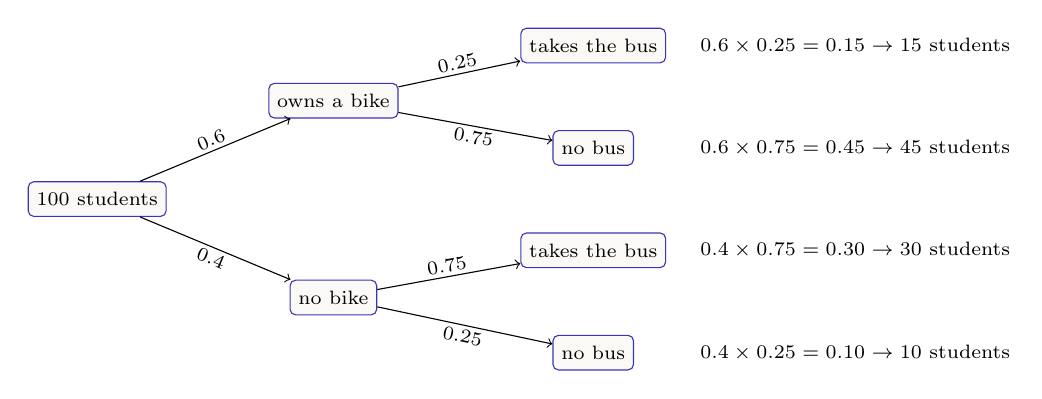
\begin{tikzpicture}[
  font=\scriptsize,
  box/.style={draw=RLBlue, fill=RLGray, rounded corners=2pt, inner sep=3pt,
              minimum height=4.4mm, align=center},
  lbl/.style={font=\scriptsize, inner sep=1.5pt}
]
  \node[box] (root) at (0,0) {100 students};
  \node[box] (bk) at (3.0,1.25) {owns a bike};
  \node[box] (nb) at (3.0,-1.25) {no bike};
  \node[box] (b1) at (6.3,1.95) {takes the bus};
  \node[box] (b2) at (6.3,0.65) {no bus};
  \node[box] (b3) at (6.3,-0.65) {takes the bus};
  \node[box] (b4) at (6.3,-1.95) {no bus};
  \draw[->] (root) -- node[lbl,above,sloped] {$0.6$} (bk);
  \draw[->] (root) -- node[lbl,below,sloped] {$0.4$} (nb);
  \draw[->] (bk) -- node[lbl,above,sloped] {$0.25$} (b1);
  \draw[->] (bk) -- node[lbl,below,sloped] {$0.75$} (b2);
  \draw[->] (nb) -- node[lbl,above,sloped] {$0.75$} (b3);
  \draw[->] (nb) -- node[lbl,below,sloped] {$0.25$} (b4);
  \node[lbl,right] at (7.6,1.95) {$0.6 \times 0.25 = 0.15 \rightarrow 15$ students};
  \node[lbl,right] at (7.6,0.65) {$0.6 \times 0.75 = 0.45 \rightarrow 45$ students};
  \node[lbl,right] at (7.6,-0.65) {$0.4 \times 0.75 = 0.30 \rightarrow 30$ students};
  \node[lbl,right] at (7.6,-1.95) {$0.4 \times 0.25 = 0.10 \rightarrow 10$ students};
\end{tikzpicture}

\vspace{0.2em}
\footnotesize The four paths cover every student exactly once, so the products sum to $1$ -- and those four counts are exactly the four cells of the table on the next slide.
\end{frame}

\begin{frame}{Worked Example: Two Socks From the Drawer}
\begin{itemize}
  \item A drawer holds $10$ socks: $6$ black and $4$ white. You pull out two in the dark.
  \pause
  \item $P(\text{1st black}) = \tfrac{6}{10}$. That sock is now gone, so $5$ black remain among $9$: $P(\text{2nd black} \mid \text{1st black}) = \tfrac59$.
  \pause
  \item Multiply along the branch: $P(\text{both black}) = \tfrac{6}{10} \times \tfrac59 = \tfrac{30}{90} = \tfrac13$.
  \pause
  \item \textbf{Why the conditioning matters:} had you put the first sock back, the draws would be independent and the answer would be $\tfrac{6}{10} \times \tfrac{6}{10} = 0.36$. Drawing without replacement makes the second draw depend on the first.
  \pause
  \item Either colour counts as a pair, and white works the same way: $\tfrac{4}{10} \times \tfrac39 = \tfrac{12}{90}$. So $P(\text{pair}) = \tfrac{30}{90} + \tfrac{12}{90} \approx 0.47$ -- less than half the time.
\end{itemize}
\end{frame}

% ─── Contingency tables ─────────────────────────────────────────────────────
\begin{frame}{Contingency Tables}
\small
A \textbf{contingency table} counts how many members of a sample fall into each combination of two attributes, with the row and column totals written in the margins.
\vspace{0.4em}

\begin{columns}[T]
\column{0.44\textwidth}
\centering
\small
\begin{tabular}{l|rr|r}
            & Bus & No bus & Total \\
\hline
Owns a bike & 15  & 45     & 60 \\
No bike     & 30  & 10     & 40 \\
\hline
Total       & 45  & 55     & 100 \\
\end{tabular}
\column{0.54\textwidth}
\small
\begin{itemize}
  \item \textbf{Joint} -- an inner cell over the grand total: $P(\text{bike} \cap \text{bus}) = \tfrac{15}{100} = 0.15$.
  \pause
  \item \textbf{Marginal} -- a margin total over the grand total: $P(\text{bus}) = \tfrac{45}{100} = 0.45$.
  \pause
  \item \textbf{Conditional} -- a cell over \emph{its own} row or column total: $P(\text{bus} \mid \text{bike}) = \tfrac{15}{60} = 0.25$.
\end{itemize}
\end{columns}
\pause
\begin{rlintuition}
Conditioning is choosing a denominator: the whole table for a joint probability, one row or column for a conditional one.
\end{rlintuition}
\end{frame}

\begin{frame}{Independence Checked From a Table}
\begin{itemize}
  \item Lecture 1 defined independence as $P(A \cap B) = P(A)P(B)$, equivalently $P(B \mid A) = P(B)$. A table turns that into a two-second check.
  \pause
  \item \textbf{Dependent:} $P(\text{bus}) = 0.45$, but $P(\text{bus} \mid \text{bike}) = 0.25$ and $P(\text{bus} \mid \text{no bike}) = 0.75$. Knowing about the bike moves the answer, so the two are \emph{not} independent.
  \pause
  \item \textbf{Independent:} in the same year group $40$ students wear glasses, and $18$ of them take the bus. $P(\text{bus} \mid \text{glasses}) = \tfrac{18}{40} = 0.45 = P(\text{bus})$ -- glasses tell you nothing about the bus.
  \pause
  \item \textbf{Shortcut for any cell:} under independence a cell should hold $\frac{\text{row total} \times \text{column total}}{n}$. That predicts $\frac{60 \times 45}{100} = 27$ bike-and-bus students, but the table says $15$; for glasses-and-bus it predicts $\frac{40 \times 45}{100} = 18$, exactly what we see.
\end{itemize}
\end{frame}

% ─── Simpson's paradox ──────────────────────────────────────────────────────
\begin{frame}{Real Event: Simpson's Paradox (Berkeley, 1973)}
\begin{columns}[T]
\column{0.42\textwidth}
\centering
\scriptsize
\begin{tabular}{l|rr|rr}
     & \multicolumn{2}{c|}{Men} & \multicolumn{2}{c}{Women} \\
Dept & applied & adm. & applied & adm. \\
\hline
A & 825 & 62\% & 108 & 82\% \\
B & 560 & 63\% &  25 & 68\% \\
C & 325 & 37\% & 593 & 34\% \\
D & 417 & 33\% & 375 & 35\% \\
E & 191 & 28\% & 393 & 24\% \\
F & 373 &  6\% & 341 &  7\% \\
\hline
\textbf{All six} & \textbf{2691} & \textbf{45\%} & \textbf{1835} & \textbf{30\%} \\
\end{tabular}

\vspace{0.4em}
{\scriptsize The six largest departments, Berkeley graduate admissions, autumn 1973.}
\column{0.56\textwidth}
\small
\begin{itemize}
  \item Pooled over all six departments, $45\%$ of the men were admitted against $30\%$ of the women -- an apparently clear gap.
  \pause
  \item Taken one department at a time the gap mostly \emph{reverses}: women were admitted at the higher rate in A, B, D and F -- four of the six.
  \pause
  \item \textbf{Why:} over half the men applied to A and B, which accepted about $64\%$ and $63\%$ of everyone who applied. Nearly three quarters of the women applied to C, E and F, which accepted $35\%$, $25\%$ and $6\%$.
  \pause
  \item Nobody's admission rate was changed by the pooling. The applicants simply were not spread evenly across easy and hard departments.
\end{itemize}
\end{columns}
\end{frame}

\begin{frame}{Simpson's Paradox: The Lesson}
\begin{itemize}
  \item $P(\text{admitted} \mid \text{woman}) < P(\text{admitted} \mid \text{man})$, and yet $P(\text{admitted} \mid \text{woman}, \text{dept})$ is the \emph{larger} of the two in most departments. Both statements are true of the same data.
  \pause
  \item Pooling groups can reverse a comparison whenever the groups differ in size \emph{and} in their underlying rates. The arithmetic is fine -- the two questions are simply not the same question.
  \pause
  \item \textbf{Everyday version:} a hospital with the worse overall survival rate can be the better hospital at every single operation, if it takes the hardest cases.
  \pause
  \item \textbf{Why this matters later:} a model fitted to pooled data can learn a relationship that holds in no subgroup at all. Always ask what the data was already conditioned on before it reached you.
\end{itemize}
\end{frame}

% \section{Lecture 2, Part 1: Bayes' Theorem}

\begin{frame}
\vfill
\centering
{\color{RLBlue}\large Lecture 2}

\vspace{0.3em}
{\color{RLBlue}\Large\bfseries Part 1}

\vspace{0.6em}
{\Large Bayes' Theorem}
\vfill
\end{frame}

\begin{frame}{Learning Goals}
\begin{itemize}
  \item Use the law of total probability to build an overall probability out of group-by-group pieces.
  \pause
  \item State Bayes' theorem, derive it from the multiplication rule, and use it to turn $P(B \mid A)$ into $P(A \mid B)$.
  \pause
  \item Name the three pieces -- prior, likelihood, posterior -- that the rest of the course reuses.
  \pause
  \item Explain why the base rate decides what a positive test result actually means.
\end{itemize}
\end{frame}

% ─── Law of total probability ───────────────────────────────────────────────
\begin{frame}{The Law of Total Probability}
\begin{rldefinition}
Split the sample space into groups $A_1, \dots, A_k$ that never overlap and together cover everything -- a \textbf{partition}, such as ``owns a bike'' and ``no bike''. Then
\[
P(B) = \sum_{i=1}^{k} P(B \mid A_i)\,P(A_i).
\]
\smallskip
\textbf{In words:} work out the chance of $B$ separately inside each group, then average those answers, weighting each group by how big it is.
\end{rldefinition}
\pause
\begin{itemize}
  \item \textbf{Students:} $P(\text{bus}) = 0.25 \times 0.6 + 0.75 \times 0.4 = 0.15 + 0.30 = 0.45$ -- exactly the $45/100$ sitting in the table's margin.
\end{itemize}
\end{frame}

\begin{frame}{Total Probability Is a Weighted Average}
\centering
\includegraphics[width=0.62\textwidth]{figures/conditional_bayes/conditional_bayes_total_probability.pdf}

\vspace{0.25em}
\footnotesize
Bar width is group size and shading is that group's bus rate, so the orange \emph{area} is the $45$ bus takers. The overall $0.45$ must land between $0.25$ and $0.75$, nearer $0.25$ because the bike group is bigger.
\end{frame}

% ─── Bayes ──────────────────────────────────────────────────────────────────
\begin{frame}{Bayes' Theorem}
\begin{rldefinition}
\textbf{Bayes' theorem} turns one conditional probability into the other:
\[
P(A \mid B) = \frac{P(B \mid A)\,P(A)}{P(B)} .
\]
\textbf{Two-line derivation:} the multiplication rule written both ways round gives $P(A \cap B) = P(A)P(B \mid A)$ and $P(A \cap B) = P(B)P(A \mid B)$; set them equal and divide by $P(B)$.
\end{rldefinition}
\pause
\begin{itemize}
  \item The denominator comes from the law of total probability: $P(B) = P(B \mid A)P(A) + P(B \mid A^c)P(A^c)$.
  \pause
  \item \textbf{Check it on the students:} $P(\text{bike} \mid \text{bus}) = \frac{0.25 \times 0.6}{0.45} = \frac{0.15}{0.45} = \tfrac13$, and the table agrees -- of the $45$ bus takers, $15$ own a bike.
\end{itemize}
\end{frame}

\begin{frame}{Prior, Likelihood, Posterior}
\begin{itemize}
  \item The three pieces of Bayes' theorem carry names that reappear in every later module:
  \begin{itemize}
    \item $P(A)$ -- the \textbf{prior}: what we believed before seeing any evidence.
    \item $P(B \mid A)$ -- the \textbf{likelihood}: how well the cause $A$ explains the evidence $B$.
    \item $P(A \mid B)$ -- the \textbf{posterior}: what we believe once we have seen it.
  \end{itemize}
  \pause
  \item \textbf{Everyday:} before looking outside, $P(\text{rain})$ is the prior. ``The pavement is wet'' is the evidence. $P(\text{wet} \mid \text{rain})$ is high, so the posterior $P(\text{rain} \mid \text{wet})$ rises -- but not to certainty, because a street cleaner also leaves wet pavement.
  \pause
  \item Bayes' theorem is the rule for updating a belief with evidence, which is exactly what learning from data means.
\end{itemize}
\end{frame}

\begin{frame}{Why Do We Need Bayes' Theorem?}
\begin{itemize}
  \item \textbf{Why:} the conditional probability we can \emph{measure} is almost always the reverse of the one we actually \emph{want}.
  \pause
  \item A test is checked on people already known to be ill, which gives $P(\text{positive} \mid \text{ill})$ -- a property of the test. The patient wants $P(\text{ill} \mid \text{positive})$, which also depends on how common the illness is.
  \pause
  \item \textbf{The two are not interchangeable:} $P(\text{wet grass} \mid \text{it rained})$ is close to $1$, while $P(\text{it rained} \mid \text{wet grass})$ is far lower -- sprinklers exist.
  \pause
  \item Same shape everywhere: a fire alarm's $P(\text{alarm} \mid \text{fire})$ versus $P(\text{fire} \mid \text{alarm})$; a filter's $P(\text{``free prize''} \mid \text{spam})$ versus $P(\text{spam} \mid \text{``free prize''})$.
\end{itemize}
\pause
\begin{rlpitfall}
Swapping the two has a name -- the \textbf{prosecutor's fallacy}. ``Only $1$ innocent person in a million would match'' is $P(\text{match} \mid \text{innocent})$, not $P(\text{innocent} \mid \text{match})$.
\end{rlpitfall}
\end{frame}

\begin{frame}{Real Event: What a Positive Test Really Means}
\begin{columns}[T]
\column{0.50\textwidth}
\small
\begin{itemize}
  \item \textbf{Base rate:} $1$ person in $100$ has the disease -- how common it is before any test. Of $10{,}000$ people, $100$ are ill and $9{,}900$ healthy.
  \pause
  \item The test \emph{never misses}: all $100$ ill test positive. But it wrongly flags $5$ in every $100$ healthy people -- $495$ more.
  \pause
  \item $100 + 495 = 595$ positives, only $100$ ill: $P(\text{ill} \mid \text{positive}) = \tfrac{100}{595} \approx \tfrac16 \approx 17\%$.
  \pause
  \item \textbf{Why:} $5\%$ of a huge group beats $100\%$ of a tiny one -- healthy people outnumber ill $99$ to $1$, so about \emph{five} false alarms per real case.
\end{itemize}
\column{0.48\textwidth}
\centering
\includegraphics[width=\linewidth]{figures/conditional_bayes/conditional_bayes_screening.pdf}
\end{columns}
\end{frame}

\begin{frame}{Why This Matters: Base Rates}
\begin{columns}[T]
\column{0.50\textwidth}
\small
\begin{itemize}
  \item Nothing about the test changes along this curve -- only how common the disease is.
  \pause
  \item At $1$ in $1000$ the same positive result means a $2\%$ chance; at $1$ in $10$ it means $69\%$.
  \pause
  \item \textbf{Why screening a healthy population is hard:} when almost everybody is well, even a small false-alarm rate produces more false positives than real cases -- so a positive screen is followed by a second, different test.
  \pause
  \item \textbf{Later in this course:} the same arithmetic is why accuracy is a useless score for rare events -- always answering ``healthy'' here would be $99\%$ accurate.
\end{itemize}
\column{0.48\textwidth}
\centering
\includegraphics[width=\linewidth]{figures/conditional_bayes/conditional_bayes_base_rate.pdf}
\end{columns}
\end{frame}

\begin{frame}{Where This Goes Next}
\begin{itemize}
  \item \textbf{Module 0, Lecture 6 -- Bayesian inference:} let $A$ be an unknown quantity and $B$ the data we collected. Bayes' theorem then updates a prior over that quantity into a posterior, and MAP estimation simply picks the posterior's peak.
  \pause
  \item \textbf{Module 3, Lecture 6 -- Naive Bayes:} classify an email by comparing $P(\text{spam})\,P(\text{words} \mid \text{spam})$ against the same product for ``not spam''. ``Naive'' means it assumes the words are independent given the class -- the independence we checked from a table today.
  \pause
  \item \textbf{Module 1, Lecture 14 -- classification metrics:} the base-rate arithmetic on the previous slide is why accuracy alone is the wrong score for a rare event.
  \pause
  \item The prior/likelihood/posterior vocabulary then reappears in generative models, in regularization, and in alignment.
\end{itemize}
\end{frame}

\begin{frame}{Summary}
\begin{itemize}
  \item $P(B \mid A) = P(A \cap B)/P(A)$: conditioning shrinks the sample space to $A$ and re-counts inside it.
  \pause
  \item Tree diagrams multiply along branches; contingency tables give joint, marginal, and conditional probabilities by changing the denominator.
  \pause
  \item Independence means the conditional equals the marginal -- and pooling groups with different rates can reverse a comparison completely (Simpson's paradox).
  \pause
  \item Law of total probability: average the group-by-group answers, weighted by group size.
  \pause
  \item Bayes' theorem reverses the conditioning. What a positive test means depends as much on the base rate as on the test itself.
\end{itemize}
\end{frame}


\section{Lecture 3, Part 0: Discrete Random Variables}

\begin{frame}
\vfill
\centering
{\color{RLBlue}\large Lecture 3}

\vspace{0.3em}
{\color{RLBlue}\Large\bfseries Part 0}

\vspace{0.6em}
{\Large Discrete Random Variables}
\vfill
\end{frame}

\begin{frame}{Learning Goals}
\begin{itemize}
  \item Write a quantity that depends on chance as a \textbf{random variable}, and list what it can be with a probability mass function.
  \pause
  \item Compute the \textbf{expectation} and \textbf{variance} of a random variable, and say how each relates to the sample mean and sample variance of Lecture 1.
  \pause
  \item Predict what happens to both when the variable is shifted or rescaled.
\end{itemize}
\end{frame}

% ─── Random variables ───────────────────────────────────────────────────────
\begin{frame}{Why Do We Need a Random Variable?}
\begin{itemize}
  \item \textbf{Why:} so far every probability has been attached to an \emph{event} -- ``the die is even'', ``the student takes the bus''. But most questions are about a \emph{number}: how many, how long, how much.
  \pause
  \item Writing ``the number of customers who buy a pastry'' in full each time is unworkable. Give it a letter, $X$, and we can add it, average it, and compare it.
  \pause
  \item \textbf{Everyday:} roll two dice and let $X$ be the sum. Rolling is chance; $X$ is the number chance produced. Board games are decided by $X$, not by which die showed what.
  \pause
  \item \textbf{Discrete} means the possible values can be listed: $0, 1, 2, \dots$ Lecture 4 does the continuous case, where they cannot.
\end{itemize}
\end{frame}

\begin{frame}{Random Variables and the Probability Mass Function}
\begin{rldefinition}
A \textbf{random variable} $X$ attaches a number to every outcome. \emph{Two dice:} the outcome is the pair $(3,4)$, and $X$, their sum, is $7$.

\smallskip
Its \textbf{probability mass function} $p(x) = P(X = x)$ lists how likely each value is. Every $p(x) \ge 0$, and they add to $1$ because $X$ must take \emph{some} value.
\end{rldefinition}
\pause
\begin{itemize}
  \item \textbf{Running example -- a coffee shop.} Let $X$ be the number of pastries in one order:
  \[
    p(0) = 0.7, \qquad p(1) = 0.2, \qquad p(2) = 0.1,
    \qquad \textstyle\sum_x p(x) = 1 .
  \]
  \pause
  \item This is the frequency distribution of Lecture 1 with one change: those were \emph{counts} from a sample we measured, these are \emph{probabilities} for a customer we have not served yet.
\end{itemize}
\end{frame}

\begin{frame}{Real Event: Why 7 Wins at Board Games}
\begin{columns}[T]
\column{0.50\textwidth}
\small
\begin{itemize}
  \item Each bar is $p(x)$; the number above it is how many of the $36$ equally likely pairs give that sum.
  \pause
  \item There is one way to roll $2$ ($1{+}1$) but six ways to roll $7$ ($1{+}6$, $2{+}5$, \dots, $6{+}1$), so $p(7) = \tfrac{6}{36} = \tfrac16$ -- six times more likely than $2$.
  \pause
  \item \textbf{Why it is a real event:} Monopoly's orange properties sit six to nine squares past Jail -- the stretch a player leaving Jail is most likely to reach -- and backgammon openings are built on the same table.
\end{itemize}
\column{0.48\textwidth}
\centering
\includegraphics[width=\linewidth]{figures/discrete_rv/discrete_rv_two_dice_pmf.pdf}
\end{columns}
\end{frame}

% ─── Expectation ────────────────────────────────────────────────────────────
\begin{frame}{Why Do We Need Expectation?}
\begin{rldefinition}
The \textbf{expectation} $E[X]$ is the average value of $X$ in the long run, with each value weighted by how likely it is:
\[
E[X] = \sum_x x\,p(x) .
\]
It is also written $\mu$ -- the same Greek letter Lecture 1 used for a population mean, because that is exactly what it is.
\end{rldefinition}
\pause
\begin{itemize}
  \item \textbf{Coffee shop:} $E[X] = 0(0.7) + 1(0.2) + 2(0.1) = 0.4$ pastries per order -- so $100$ customers should buy about $40$ pastries.
  \pause
  \item \textbf{Note:} $0.4$ is not a possible order. An expectation is a long-run average, not a prediction of any single case -- like ``$1.8$ children per family''.
\end{itemize}
\end{frame}

\begin{frame}{Worked Example: Is the Raffle Ticket Worth It?}
\begin{itemize}
  \item A school sells $500$ raffle tickets at \$2 each. One ticket wins a \$400 bicycle.
  \pause
  \item Let $X$ be your \emph{net} gain. You either win the bicycle having paid \$2, or you just lose the \$2:
  \[
    p(398) = \tfrac{1}{500}, \qquad p(-2) = \tfrac{499}{500}.
  \]
  \pause
  \item $E[X] = 398 \cdot \tfrac{1}{500} - 2 \cdot \tfrac{499}{500} = \tfrac{398 - 998}{500} = -\tfrac{600}{500} = -\$1.20$.
  \pause
  \item \textbf{Reading it:} every ticket costs the buyer \$1.20 on average, and the school keeps \$600 of the \$1000 raised. No single buyer ever loses \$1.20 -- they lose \$2 or win \$398 -- yet the school can budget on it exactly.
\end{itemize}
\end{frame}

\begin{frame}{Expectation Is Where the Sample Mean Lands}
\begin{columns}[T]
\column{0.50\textwidth}
\small
\begin{itemize}
  \item Lecture 1's $\bar{x}$ was computed \emph{from data we had}. $E[X]$ is a property of the \emph{process}, fixed before any data exists.
  \pause
  \item Roll a die again and again, keeping the running $\bar{x}$. Three independent runs wander at first, then settle on $E[X] = 3.5$.
  \pause
  \item After $10$ rolls the three runs read $4.10$, $3.60$, $3.90$; after $2000$ they read $3.54$, $3.51$, $3.49$.
  \pause
  \item \textbf{Why this matters:} it is why measuring more data helps at all. Lecture 5 makes the rate precise -- the law of large numbers and the CLT.
\end{itemize}
\column{0.48\textwidth}
\centering
\includegraphics[width=\linewidth]{figures/discrete_rv/discrete_rv_running_mean.pdf}
\end{columns}
\end{frame}

% ─── Variance ───────────────────────────────────────────────────────────────
\begin{frame}{Why Do We Need the Variance of a Random Variable?}
\begin{rldefinition}
The \textbf{variance} is the expected squared distance from the mean, written $\sigma^2$:
\[
\mathrm{Var}(X) = E\!\left[(X - \mu)^2\right] = E[X^2] - \mu^2 ,
\qquad \sigma = \sqrt{\mathrm{Var}(X)} .
\]
The second form is the one to compute with: square the values, average them, subtract the square of the mean.
\end{rldefinition}
\pause
\begin{itemize}
  \item \textbf{Coffee shop:} $E[X^2] = 0^2(0.7) + 1^2(0.2) + 2^2(0.1) = 0.6$, so $\mathrm{Var}(X) = 0.6 - 0.4^2 = 0.44$ and $\sigma \approx 0.66$.
  \pause
  \item Same idea as Lecture 1's $s^2$, and same reason: the mean alone cannot tell a steady process from an erratic one.
\end{itemize}
\end{frame}

\begin{frame}{Worked Example: Two Raffles, Same Expectation}
\begin{itemize}
  \item \textbf{Raffle A} (from the previous slide): one \$400 prize among $500$ tickets, $E[X] = -\$1.20$.
  \pause
  \item \textbf{Raffle B}: same $500$ tickets at \$2, but \emph{fifty} \$8 prizes. Net gain is $+\$6$ with probability $\tfrac{50}{500} = 0.1$, else $-\$2$:
  $E[X] = 6(0.1) - 2(0.9) = -\$1.20$ -- \emph{identical}.
  \pause
  \item But $\mathrm{Var}_A = 320.8 - 1.44 = 319.36$, giving $\sigma_A \approx \$17.87$, while $\mathrm{Var}_B = 7.2 - 1.44 = 5.76$, giving $\sigma_B = \$2.40$.
  \pause
  \item \textbf{Why:} the expectation says what the school raises; the variance says what the \emph{buyer} experiences. Raffle A is a lottery, Raffle B is a mild discount -- and no expectation can tell them apart.
\end{itemize}
\end{frame}

\begin{frame}{Shifting and Scaling}
\begin{rldefinition}
For constants $a$ and $b$:
\[
E[aX + b] = a\,E[X] + b ,
\qquad
\mathrm{Var}(aX + b) = a^2\,\mathrm{Var}(X) .
\]
Adding $b$ moves the whole distribution without stretching it, so the spread is untouched; the $a^2$ appears because variance is measured in squared units.
\end{rldefinition}
\pause
\begin{itemize}
  \item \textbf{Coffee shop:} a pastry costs \$2, so pastry revenue is $R = 2X$ with $E[R] = \$0.80$ and $\sigma_R = 2(0.66) = \$1.33$.
  \pause
  \item Every order also includes a \$3 coffee, so the bill is $T = 2X + 3$: $E[T] = \$3.80$, and $\mathrm{Var}(T) = 1.76$ -- exactly $\mathrm{Var}(R)$, because a fixed \$3 adds no uncertainty.
\end{itemize}
\end{frame}

% ═══════════════════════════════════════════════════════════════════════════

\section{Lecture 3, Part 1: Key Distributions}

\begin{frame}
\vfill
\centering
{\color{RLBlue}\large Lecture 3}

\vspace{0.3em}
{\color{RLBlue}\Large\bfseries Part 1}

\vspace{0.6em}
{\Large Key Distributions}
\vfill
\end{frame}

\begin{frame}{Learning Goals}
\begin{itemize}
  \item Recognize the Bernoulli, Binomial, Categorical, and Multinomial distributions from the question being asked.
  \pause
  \item Use the Poisson distribution for counts of events in a fixed window, and say when it replaces the Binomial.
  \pause
  \item Explain what a Dirichlet distribution is a distribution \emph{over}, and why that is useful.
\end{itemize}
\end{frame}

\begin{frame}{Why Do We Need Named Distributions?}
\begin{itemize}
  \item \textbf{Why:} the same handful of shapes keep reappearing. Once a situation is recognized as one of them, the whole PMF, its expectation, and its variance come for free -- no counting required.
  \pause
  \item Four everyday questions, four different shapes:
  \begin{itemize}
    \item Did \emph{this one} customer buy a pastry? -- \textbf{Bernoulli}
    \item How many of the next \emph{ten} did? -- \textbf{Binomial}
    \item Which \emph{size} of cup did this customer pick? -- \textbf{Categorical}
    \item How many customers walk in during the next \emph{ten minutes}? -- \textbf{Poisson}
  \end{itemize}
  \pause
  \item A named distribution is also a claim about the world, and it can be wrong -- which is why the last one gets checked against real counts.
\end{itemize}
\end{frame}

% ─── Bernoulli & Binomial ───────────────────────────────────────────────────
\begin{frame}{Bernoulli: One Yes-or-No Trial}
\begin{rldefinition}
A \textbf{Bernoulli} variable takes the value $1$ with probability $p$ and $0$ otherwise -- a single yes/no question. \emph{A coin:} $p = 0.5$. \emph{A newborn being a girl:} $p \approx 0.49$.
\[
E[Y] = p, \qquad \mathrm{Var}(Y) = p(1-p).
\]
\end{rldefinition}
\pause
\begin{itemize}
  \item \textbf{From Part 0:} let $Y = 1$ if the order contains \emph{any} pastry. Then $p = p(1) + p(2) = 0.2 + 0.1 = 0.3$, so $E[Y] = 0.3$ and $\mathrm{Var}(Y) = 0.3 \times 0.7 = 0.21$.
  \pause
  \item The spread is largest at $p = 0.5$ and vanishes at $p = 0$ or $1$: a question whose answer is already known carries no uncertainty.
\end{itemize}
\end{frame}

\begin{frame}{Binomial: Counting Successes in $n$ Trials}
\begin{rldefinition}
Repeat the same Bernoulli trial $n$ times, independently, and count the successes. That count is \textbf{Binomial}$(n, p)$:
\[
P(X = k) = \binom{n}{k} p^k (1-p)^{n-k},
\qquad E[X] = np, \qquad \mathrm{Var}(X) = np(1-p).
\]
The $\binom{n}{k}$ counts the orders in which those $k$ successes could arrive; $p^k(1-p)^{n-k}$ is the probability of any one such order.
\end{rldefinition}
\pause
\begin{itemize}
  \item \textbf{Both conditions matter:} the same $p$ every time, and no trial affecting another. Drawing socks without replacement in Lecture 2 broke the second, which is why that answer was not binomial.
\end{itemize}
\end{frame}

\begin{frame}{Real Event: How Many of the Next Ten Buy a Pastry?}
\begin{columns}[T]
\column{0.50\textwidth}
\small
\begin{itemize}
  \item Ten customers, each buying a pastry with probability $p = 0.3$: $X \sim$ Binomial$(10, 0.3)$.
  \pause
  \item $P(X = 3) = \binom{10}{3}(0.3)^3(0.7)^7 = 120 \times 0.027 \times 0.0824 \approx 0.267$ -- the single most likely count, and it happens only about once in four batches.
  \pause
  \item $E[X] = 10 \times 0.3 = 3$, $\sigma = \sqrt{2.1} \approx 1.45$.
  \pause
  \item \textbf{Why the baker cares:} baking exactly three is wrong most of the time. $P(X \ge 6) \approx 0.047$ -- roughly one batch in twenty sells out at six or more.
\end{itemize}
\column{0.48\textwidth}
\centering
\includegraphics[width=\linewidth]{figures/discrete_rv/discrete_rv_binomial.pdf}
\end{columns}
\end{frame}

% ─── Categorical & Multinomial ──────────────────────────────────────────────
\begin{frame}{Categorical and Multinomial: More Than Two Options}
\begin{rldefinition}
A \textbf{Categorical} variable picks one of $k$ options, with probabilities $p_1, \dots, p_k$ that add to $1$ -- a Bernoulli with more than two answers. \emph{Cup size:} small $0.2$, medium $0.5$, large $0.3$.

\smallskip
A \textbf{Multinomial} counts how many of $n$ independent picks landed in each option -- a Binomial with more than two answers. Expected counts are $n p_i$.
\end{rldefinition}
\pause
\begin{itemize}
  \item \textbf{Ten customers:} expect $2$ small, $5$ medium, $3$ large -- but any single morning will differ, exactly as the Binomial bars showed.
  \pause
  \item \textbf{Later in this course:} a classifier's output layer produces $p_1, \dots, p_k$ that add to $1$ -- that is the softmax, and it is a Categorical distribution over the classes.
\end{itemize}
\end{frame}

% ─── Poisson ────────────────────────────────────────────────────────────────
\begin{frame}{Poisson: Counting Events in a Window}
\begin{rldefinition}
The \textbf{Poisson} distribution counts how many events land in a fixed window of time or space, when they arrive independently at an average rate $\lambda$ per window:
\[
P(X = k) = \frac{e^{-\lambda}\lambda^{k}}{k!},
\qquad E[X] = \lambda, \qquad \mathrm{Var}(X) = \lambda .
\]
\emph{Everyday:} calls to a help desk per hour, buses arriving per ten minutes, typos per page.
\end{rldefinition}
\pause
\begin{itemize}
  \item There is no ``$n$'' here: we never count the customers who \emph{did not} walk in. That is the practical difference from the Binomial.
  \pause
  \item \textbf{The mean equals the variance} -- a strong, checkable claim, and the first thing to test on real counts.
\end{itemize}
\end{frame}

\begin{frame}{Real Event: Arrivals at the Coffee Shop}
\begin{columns}[T]
\column{0.50\textwidth}
\small
\begin{itemize}
  \item Customers arrive independently at $\lambda = 4$ per ten minutes. Bars are $3000$ observed windows; dots are the Poisson formula.
  \pause
  \item Observed mean $3.96$, variance $3.84$ -- close to each other and to $\lambda$, as Poisson requires.
  \pause
  \item $P(X = 0) = e^{-4} \approx 0.018$: one window in $55$ is empty. $P(X \ge 8) \approx 0.051$: one in twenty is a rush.
  \pause
  \item \textbf{Why staffing needs this:} a ten-hour day holds $60$ windows, so four on average still brings about three rushes.
\end{itemize}
\column{0.48\textwidth}
\centering
\includegraphics[width=\linewidth]{figures/discrete_rv/discrete_rv_poisson.pdf}
\end{columns}
\end{frame}

\begin{frame}{Binomial or Poisson?}
\begin{itemize}
  \item \textbf{Binomial} when there is a fixed number of trials and both outcomes are visible: $10$ customers, each buys or does not.
  \pause
  \item \textbf{Poisson} when only the events are visible and the window is what is fixed: customers arriving, with no count of the people who stayed home.
  \pause
  \item \textbf{They meet:} split the ten minutes into $600$ seconds, each with a tiny $p = \tfrac{1}{150}$ chance of an arrival. Then $np = 4$, and Binomial$(600, \tfrac{1}{150})$ agrees with Poisson$(4)$ to within $0.001$ at every count.
  \pause
  \item \textbf{So:} the Poisson is what the Binomial becomes when $n$ is huge, $p$ is tiny, and only the product $np = \lambda$ matters.
\end{itemize}
\end{frame}

% ─── Dirichlet ──────────────────────────────────────────────────────────────
\begin{frame}{Why Do We Need a Distribution Over the Shares?}
\begin{itemize}
  \item Every distribution so far assumed we \emph{know} $p_1, \dots, p_k$. We never do. The cup-size shares $0.2, 0.5, 0.3$ came from counting a few mornings' orders.
  \pause
  \item \textbf{Numerical example:} the first four orders were $1$ small, $2$ medium, $1$ large. Read literally that says the shares are $0.25, 0.50, 0.25$ -- but with only four orders nobody would be surprised if the truth were $0.10, 0.60, 0.30$, or $0.40, 0.40, 0.20$.
  \pause
  \item So the shares themselves are uncertain, and we need a way to say \emph{which sets of shares are plausible} -- not one answer, but a spread of answers.
  \pause
  \item That is awkward, because the answer is three numbers at once and they must always add to $1$. A distribution over a single number will not do it.
\end{itemize}
\end{frame}

\begin{frame}{The Dirichlet: A Distribution Over the Bar Heights}
\begin{columns}[T]
\column{0.50\textwidth}
\small
\begin{itemize}
  \item A \textbf{Dirichlet} draws a whole set of shares at once, always adding to $1$. Each thin line is one draw.
  \pause
  \item Its parameter $\alpha$ counts \textbf{orders already seen}. Top: $(0.8, 2, 1.2)$, about four -- wide scatter. Bottom: $(8, 20, 12)$, about forty -- tight.
  \pause
  \item \textbf{Updating is counting:} three more mediums, add $3$ to the middle entry.
  \pause
  \item \textbf{In AI:} a softmax gives shares with no sense of how sure it is; predict $\alpha$ instead and the network can say ``I have barely seen this'' -- the idea behind LDA (Module 3) and AlphaZero's move priors (Module 5).
\end{itemize}
\column{0.48\textwidth}
\centering
\includegraphics[width=0.96\linewidth]{figures/discrete_rv/discrete_rv_dirichlet.pdf}
\end{columns}
\end{frame}

\begin{frame}{Where This Goes Next}
\begin{itemize}
  \item \textbf{Lecture 4 -- continuous random variables:} the same ideas when the values cannot be listed. The bars become a curve and the sum becomes an integral.
  \pause
  \item \textbf{Lecture 5 -- CLT and maximum likelihood:} the Binomial and Bernoulli are the first distributions we will fit to data, and Bernoulli likelihood is exactly the cross-entropy loss.
  \pause
  \item \textbf{Lecture 6 -- Bayesian inference:} the Dirichlet becomes the prior over a Categorical, updated by counts into a posterior.
  \pause
  \item \textbf{Lecture 7 -- information theory:} entropy measures how uncertain one of these distributions is, in bits.
\end{itemize}
\end{frame}

\begin{frame}{Summary}
\begin{itemize}
  \item A random variable turns an outcome into a number; its PMF lists the values and their probabilities, and they sum to $1$.
  \pause
  \item $E[X] = \sum_x x\,p(x)$ is the population version of Lecture 1's $\bar{x}$; $\mathrm{Var}(X) = E[X^2] - \mu^2$ is the population version of $s^2$. Shifting leaves the variance alone; scaling by $a$ multiplies it by $a^2$.
  \pause
  \item Bernoulli for one yes/no trial, Binomial for successes in $n$ of them; Categorical and Multinomial are the same pair with more than two options.
  \pause
  \item Poisson counts events in a window at rate $\lambda$, with mean and variance both equal to $\lambda$ -- and it is the Binomial's limit when $n$ is large and $p$ small.
  \pause
  \item A Dirichlet is a distribution over a Categorical's probabilities -- uncertainty about the shape itself.
\end{itemize}
\end{frame}


% \section{Lecture 4, Part 0: Continuous Random Variables}

\begin{frame}
\vfill
\centering
{\color{RLBlue}\large Lecture 4}

\vspace{0.3em}
{\color{RLBlue}\Large\bfseries Part 0}

\vspace{0.6em}
{\Large Continuous Random Variables}
\vfill
\end{frame}

\begin{frame}{Learning Goals}
\begin{itemize}
  \item Say why a continuous quantity needs a \textbf{density} rather than a probability for each value, and read probability as \emph{area}.
  \pause
  \item Use the CDF to answer ``at most'', ``at least'' and ``between'' questions.
  \pause
  \item Recognize the uniform, exponential and Beta distributions from the question being asked.
\end{itemize}
\end{frame}

% ─── Why a density ──────────────────────────────────────────────────────────
\begin{frame}{Why Do We Need a Density Instead of a Probability?}
\begin{itemize}
  \item \textbf{Why:} Lecture 3 listed the values a variable could take. Now take the \emph{gap} between two customers walking into the coffee shop. Between $2$ and $3$ minutes there are already infinitely many possible answers -- $2.5$, $2.51$, $2.500\overline{7}$ -- so they cannot be listed.
  \pause
  \item \textbf{The awkward consequence:} if infinitely many values each had a probability above zero, the total would exceed $1$. So for a continuous variable
  \[
    P(X = 2.5 \text{ exactly}) = 0 ,
  \]
  and that is not a trick -- no stopwatch ever reads exactly $2.5$.
  \pause
  \item \textbf{The fix:} stop asking for single values and ask for \emph{ranges}. $P(2 < X < 3)$ is a perfectly good number. The object that answers range questions is a \textbf{density}.
\end{itemize}
\end{frame}

\begin{frame}{From Bars to a Curve}
\begin{columns}[T]
\column{0.50\textwidth}
\small
\begin{itemize}
  \item $20{,}000$ observed gaps between customers, drawn as the histogram of Lecture 1 -- but with the vertical axis rescaled so that \emph{total area is $1$}.
  \pause
  \item Top: bins $2$ minutes wide, six bars. Bottom: bins $0.25$ minutes wide, forty-eight bars.
  \pause
  \item Keep shrinking the bins and the bar tops stop being bars. What they trace out is the blue curve -- the \textbf{density}.
  \pause
  \item \textbf{Nothing changed but the resolution.} A density is the shape a histogram settles into when the bins get arbitrarily narrow and the data arbitrarily plentiful.
\end{itemize}
\column{0.48\textwidth}
\centering
\includegraphics[width=\linewidth]{figures/continuous_gaussian/continuous_histogram_to_density.pdf}
\end{columns}
\end{frame}

\begin{frame}{The Probability Density Function}
\begin{rldefinition}
A \textbf{probability density function} $f(x)$ gives probability as \emph{area}: the chance of landing between $a$ and $b$ is the area under $f$ from $a$ to $b$.
\[
P(a < X < b) = \int_a^b f(x)\,\mathrm{d}x,
\qquad f(x) \ge 0,
\qquad \int_{-\infty}^{\infty} f(x)\,\mathrm{d}x = 1 .
\]
\emph{Reading the integral sign:} it is the $\sum$ of Lecture 3 with the bars made infinitely thin -- ``add up the area''.
\end{rldefinition}
\pause
\begin{itemize}
  \item \textbf{$f(x)$ is not a probability} and may exceed $1$: a delivery landing uniformly within a $30$-second window has density $1/0.5 = 2$ per minute. Think of $f(x)$ as concentration -- probability per minute -- the way speed is distance per hour.
\end{itemize}
\end{frame}

\begin{frame}{Real Event: How Long Until the Next Customer?}
\begin{columns}[T]
\column{0.50\textwidth}
\small
\begin{itemize}
  \item Lecture 3 had $4$ arrivals per ten minutes. So the average gap is $2.5$ minutes, and the density of the gap is $f(x) = 0.4\,e^{-0.4x}$.
  \pause
  \item \textbf{Will the next customer arrive within $2$ minutes?} Shade the area from $0$ to $2$:
  $P(X < 2) = 1 - e^{-0.8} = 0.55$.
  \pause
  \item The lower panel stacks that area up as you sweep left to right. At $x = 2$ its height is $0.55$ -- the same number, read off a curve instead of measured as an area.
  \pause
  \item \textbf{Why the barista cares:} a quiet stretch of $5$ minutes or more still happens $e^{-2} = 13.5\%$ of the time, so a lull is no sign the rush is over.
\end{itemize}
\column{0.48\textwidth}
\centering
\includegraphics[width=\linewidth]{figures/continuous_gaussian/continuous_density_and_cdf.pdf}
\end{columns}
\end{frame}

\begin{frame}{The CDF: Everything Up To Here}
\begin{rldefinition}
The \textbf{cumulative distribution function} $F(x) = P(X \le x)$ is the area under the density to the \emph{left} of $x$ -- the running total. It starts at $0$, ends at $1$, and never decreases. \emph{Gaps between customers:} $F(2) = 0.55$, so $55\%$ of gaps are under two minutes.
\end{rldefinition}
\pause
\begin{itemize}
  \item Every range question is two lookups and a subtraction:
  \[
    P(a < X < b) = F(b) - F(a) .
  \]
  \pause
  \item \textbf{Worked example:} gaps between $2$ and $5$ minutes. $F(5) = 1 - e^{-2} = 0.865$ and $F(2) = 0.551$, so the answer is $0.865 - 0.551 = 0.314$ -- just under a third.
  \pause
  \item This is why tables and software report $F$, not $f$: $F$ is what actually answers questions.
\end{itemize}
\end{frame}

% ─── Uniform and exponential ────────────────────────────────────────────────
\begin{frame}{Uniform and Exponential: The Two Simplest Shapes}
\begin{columns}[T]
\column{0.50\textwidth}
\small
\begin{itemize}
  \item \textbf{Uniform}$(a,b)$ -- every value equally likely, density flat at $1/(b-a)$. \emph{A delivery promised ``within ten minutes''}: $f(x) = 0.1$, so it lands in the first three minutes with probability $3/10$.
  \pause
  \item \textbf{Exponential}$(\lambda)$ -- the wait until the next event when events arrive at rate $\lambda$: $f(x) = \lambda e^{-\lambda x}$, mean $1/\lambda$.
  \pause
  \item The shapes say opposite things: under the uniform no moment is special; under the exponential short waits are always commonest, however long you have already waited.
\end{itemize}
\column{0.48\textwidth}
\centering
\includegraphics[width=\linewidth]{figures/continuous_gaussian/continuous_uniform_exponential.pdf}
\end{columns}
\end{frame}

\begin{frame}{Why Does the Exponential Pair With the Poisson?}
\begin{itemize}
  \item They are two views of one process. \textbf{Poisson} counts how many customers arrive in ten minutes; \textbf{exponential} measures the gap between consecutive arrivals. Rate $\lambda = 4$ per ten minutes $\Rightarrow$ mean gap $2.5$ minutes.
  \pause
  \item \textbf{The memoryless property:} having already waited three minutes changes nothing.
  \[
    P(X > 5 \mid X > 3) = \frac{e^{-2}}{e^{-1.2}} = e^{-0.8} = 0.449 = P(X > 2) .
  \]
  \pause
  \item \textbf{Everyday reading:} the shop does not ``owe'' you a customer. The queue has no memory of the quiet stretch -- which is exactly the independence assumption the Poisson made in Lecture 3.
  \pause
  \item \textbf{And a warning:} that is a strong claim about the world. Real arrivals cluster at lunchtime, and then neither model fits.
\end{itemize}
\end{frame}

\begin{frame}{Why This Matters: Every Random Number Starts Uniform}
\begin{itemize}
  \item A computer can only produce one kind of randomness: a uniform number between $0$ and $1$. Everything else is built from it by running a CDF \emph{backwards}.
  \pause
  \item \textbf{Worked example.} Draw $u \sim$ Uniform$(0,1)$ and solve $F(x) = u$. For the exponential, $1 - e^{-\lambda x} = u$ gives
  \[
    x = -\frac{\ln(1-u)}{\lambda} .
  \]
  With $u = 0.5$ and $\lambda = 0.4$: $x = 1.73$ minutes -- and indeed half of all gaps are shorter than that.
  \pause
  \item \textbf{Why an AI course teaches this:} this is how sampling actually happens. Dropout masks, shuffled mini-batches, data augmentation and the noise added at every step of a diffusion model all begin as uniform draws pushed through an inverse CDF.
\end{itemize}
\end{frame}

% ─── Beta ───────────────────────────────────────────────────────────────────
\begin{frame}{Why Do We Need a Distribution Over One Probability?}
\begin{itemize}
  \item Lecture 3 ended with the same problem for \emph{many} categories: the Dirichlet, a distribution over the cup-size shares. The two-outcome case deserves its own name.
  \pause
  \item \textbf{The question:} what fraction $p$ of customers buy a pastry? Lecture 3 simply asserted $p = 0.3$. Where did that come from, and how sure are we?
  \pause
  \item \textbf{Numerical example:} $3$ of the first $10$ orders included a pastry. Read literally that is $p = 0.30$ -- but $0.20$ or $0.45$ would hardly be surprising on ten orders.
  \pause
  \item So $p$ itself is an unknown number between $0$ and $1$, and we need a density over exactly that range.
\end{itemize}
\end{frame}

\begin{frame}{The Beta: A Belief About a Single Rate}
\begin{columns}[T]
\column{0.50\textwidth}
\small
\begin{itemize}
  \item A \textbf{Beta}$(\alpha, \beta)$ is a density on $[0,1]$, so it can only describe a proportion; its mean is $\alpha/(\alpha+\beta)$.
  \pause
  \item Like the Dirichlet, $\alpha$ and $\beta$ \textbf{count successes and failures}. Top: $3$ of $10$, Beta$(4,8)$, mean $0.33 \pm 0.13$. Bottom: $30$ of $100$, Beta$(31,71)$, mean $0.30 \pm 0.05$. \textbf{Updating is counting:} one more pastry adds $1$ to $\alpha$.
  \pause
  \item \textbf{In AI:} this is how a click-rate or a model's accuracy is tracked as evidence arrives -- $12$ correct of $15$ is not the evidence $800$ of $1000$ is. Lecture 6 makes it the conjugate prior for a Bernoulli.
\end{itemize}
\column{0.48\textwidth}
\centering
\includegraphics[width=0.96\linewidth]{figures/continuous_gaussian/continuous_beta.pdf}
\end{columns}
\end{frame}

% \section{Lecture 4, Part 1: The Gaussian}

\begin{frame}
\vfill
\centering
{\color{RLBlue}\large Lecture 4}

\vspace{0.3em}
{\color{RLBlue}\Large\bfseries Part 1}

\vspace{0.6em}
{\Large The Gaussian}
\vfill
\end{frame}

\begin{frame}{Learning Goals}
\begin{itemize}
  \item State the normal distribution's two parameters and use the $68$--$95$--$99.7$ rule without a table.
  \pause
  \item Convert any measurement to a \textbf{z-score} and use it to compare quantities measured on different scales.
  \pause
  \item Read a \textbf{mean vector} and \textbf{covariance matrix}, and say what the contour ellipses of a multivariate Gaussian show.
\end{itemize}
\end{frame}

% ─── The normal distribution ────────────────────────────────────────────────
\begin{frame}{Why Do We Need the Gaussian?}
\begin{itemize}
  \item \textbf{Why:} because it keeps turning up unbidden. Weigh croissants, measure heights, read a thermometer twice -- the same bell shape appears, whatever the underlying mechanism.
  \pause
  \item \textbf{The reason, in one line:} anything built by \emph{adding up} many small independent wobbles ends up Gaussian. A croissant's weight is dough portioning, plus flour moisture, plus oven position, plus rise time, plus a dozen others.
  \pause
  \item That is the Central Limit Theorem, and Lecture 5 proves it. For now take the consequence: sums and averages drift toward this one shape, so it is worth knowing in detail.
  \pause
  \item \textbf{Everyday consequence:} two numbers -- a centre and a spread -- are enough to answer almost any question about the whole batch.
\end{itemize}
\end{frame}

\begin{frame}{The Normal Distribution}
\begin{rldefinition}
A \textbf{normal} (or \textbf{Gaussian}) variable $X \sim \mathcal{N}(\mu, \sigma^2)$ has the symmetric bell-shaped density
\[
f(x) = \frac{1}{\sigma\sqrt{2\pi}}\,
        \exp\!\left(-\frac{(x-\mu)^2}{2\sigma^2}\right).
\]
$\mu$ slides the curve sideways, $\sigma$ stretches it. \emph{The bakery's croissants:} $\mu = 60$\,g, $\sigma = 2$\,g.
\end{rldefinition}
\pause
\begin{itemize}
  \item The formula is never needed by hand -- it has no closed-form integral. What is needed is the consequence below.
  \pause
  \item \textbf{The $68$--$95$--$99.7$ rule:} about $68\%$ of the batch lies within $1\sigma$ of $\mu$, about $95\%$ within $2\sigma$, and about $99.7\%$ within $3\sigma$. Exactly: $68.27\%$, $95.45\%$, $99.73\%$.
\end{itemize}
\end{frame}

\begin{frame}{Real Event: Croissant Weights and the $68$--$95$--$99.7$ Rule}
\begin{columns}[T]
\column{0.50\textwidth}
\small
\begin{itemize}
  \item Target $60$\,g, $\sigma = 2$\,g. The rule reads straight off the axis: $68\%$ weigh between $58$ and $62$\,g, $95\%$ between $56$ and $64$\,g, $99.7\%$ between $54$ and $66$\,g.
  \pause
  \item \textbf{Why the bakery cares:} the label promises ``$55$\,g or more''. That is $2.5\sigma$ below target, so the shortfall rate is $0.62\%$ -- about $6$ croissants in every $1000$.
  \pause
  \item Tighten the process to $\sigma = 1.5$\,g and $55$\,g becomes $3.3\sigma$ away: about $4$ per $10{,}000$. \textbf{Spread, not the average, decides the failure rate} -- the same lesson as Lecture 1's bottling line, now with a formula behind it.
\end{itemize}
\column{0.48\textwidth}
\centering
\includegraphics[width=\linewidth]{figures/continuous_gaussian/gaussian_empirical_rule.pdf}
\end{columns}
\end{frame}

% ─── z-scores ───────────────────────────────────────────────────────────────
\begin{frame}{Why Do We Need z-scores?}
\begin{rldefinition}
The \textbf{z-score} of a measurement is how many standard deviations it sits from the mean, $z = (x - \mu)/\sigma$. It has no units, so grams and minutes become comparable. \emph{A $57$\,g croissant:} $z = (57-60)/2 = -1.5$, one and a half standard deviations light.
\end{rldefinition}
\pause
\begin{itemize}
  \item \textbf{Worked example -- which bake went further wrong?} One morning a croissant came out at $57$\,g and a loaf at $480$\,g, where loaves are $\mathcal{N}(500, 15^2)$:
  \[
    z_{\text{croissant}} = \tfrac{-3}{2} = -1.50,
    \qquad
    z_{\text{loaf}} = \tfrac{-20}{15} = -1.33 .
  \]
  \pause
  \item The loaf is $20$\,g light and the croissant only $3$\,g, yet the \emph{croissant} is the more unusual bake: $6.7\%$ of croissants come out that light against $9.1\%$ of loaves. Raw differences mislead; z-scores do not.
\end{itemize}
\end{frame}

\begin{frame}{Why This Matters: Standardizing Is Everywhere}
\begin{itemize}
  \item Subtracting $\mu$ and dividing by $\sigma$ turns any measurement into ``how many spreads from typical''. Doing that to every column of a table is called \textbf{standardizing}.
  \pause
  \item \textbf{Why an AI course teaches this:} k-NN measures distances, so a column in grams and a column in kilograms would count a thousand times differently -- standardize first and they do not (Module 1, Lecture 1). PCA has the same problem, for the same reason (Module 1, Lecture 2).
  \pause
  \item \textbf{And inside the network:} \textbf{batch normalization} takes the z-score of each activation using the mean and standard deviation of the current mini-batch. It is this slide's formula applied a few hundred times per forward pass (Module 2, Lecture 6).
\end{itemize}
\end{frame}

% ─── Multivariate ───────────────────────────────────────────────────────────
\begin{frame}{Why Do We Need More Than One Number at a Time?}
\begin{itemize}
  \item Real records come in bundles. For each trading day the shop notes the high temperature \emph{and} the iced coffees sold -- and those two are plainly not independent.
  \pause
  \item Describing them separately (``temperature averages $22^\circ$C, sales average $40$ cups'') throws away the very thing worth knowing: warm days sell more.
  \pause
  \item \textbf{What is missing is a number for moving together.} Variance measured how one quantity spreads; we now need how two co-spread. That number is the \textbf{covariance}, and with $k$ quantities it becomes a $k \times k$ matrix.
\end{itemize}
\end{frame}

\begin{frame}{The Multivariate Gaussian}
\begin{rldefinition}
A \textbf{multivariate Gaussian} replaces $\mu$ with a \textbf{mean vector} $\boldsymbol{\mu}$ -- one typical value per quantity -- and $\sigma^2$ with a \textbf{covariance matrix} $\Sigma$. $\Sigma_{ii}$ is the variance of quantity $i$; $\Sigma_{ij}$ is their covariance: positive when they rise together, negative when one rises as the other falls, zero when knowing one says nothing about the other.
\end{rldefinition}
\pause
\begin{itemize}
  \item \textbf{From $300$ trading days} (temperature in $^\circ$C, iced coffees sold):
  \[
    \boldsymbol{\mu} = \begin{pmatrix} 21.8 \\ 39.5 \end{pmatrix},
    \qquad
    \Sigma = \begin{pmatrix} 31.9 & 49.6 \\ 49.6 & 128.4 \end{pmatrix}.
  \]
  \pause
  \item Read it: temperature varies with $\sqrt{31.9} = 5.7^\circ$C, sales with $\sqrt{128.4} = 11.3$ cups, and the off-diagonal $49.6$ is positive -- warm days sell more. Dividing out both spreads gives the correlation, $49.6/(5.7 \times 11.3) = 0.77$.
\end{itemize}
\end{frame}

\begin{frame}{Real Event: Hot Days and Iced Coffee}
\begin{columns}[T]
\column{0.50\textwidth}
\small
\begin{itemize}
  \item Each dot is one trading day; the ellipses are the $1\sigma$ and $2\sigma$ contours.
  \pause
  \item \textbf{The tilt is the covariance.} Zero covariance lines the ellipses up with the axes; positive covariance tips them upward, and stronger correlation makes them thinner.
  \pause
  \item \textbf{Why the ellipse is the useful object:} the starred day, $28^\circ$C and only $25$ cups, sits well outside it -- yet $28^\circ$C is just $1.1$ standard deviations warm and $25$ cups $1.3$ light. Only the \emph{pair} is strange, $3.5$ standard deviations out; checking each column alone would have missed it.
\end{itemize}
\column{0.48\textwidth}
\centering
\includegraphics[width=\linewidth]{figures/continuous_gaussian/gaussian_bivariate.pdf}
\end{columns}
\end{frame}

\begin{frame}{Why an AI Course Spends a Lecture on One Curve}
\begin{itemize}
  \item \textbf{The long axis of that ellipse is what PCA finds.} PCA diagonalizes the covariance matrix: its principal directions \emph{are} the ellipse's axes, and the variance along each is how far the ellipse stretches (Module 1, Lecture 2).
  \pause
  \item \textbf{Clustering.} A Gaussian Mixture Model describes data as several of these ellipses overlaid -- one per cluster, each with its own $\boldsymbol{\mu}$ and $\Sigma$ (Module 1, Lecture 9).
  \pause
  \item \textbf{Starting a network.} Weights are initialized by drawing from $\mathcal{N}(0, \sigma^2)$ with $\sigma$ set by the layer width, precisely so activations neither vanish nor explode (Module 2).
  \pause
  \item \textbf{Regularization is a Gaussian in disguise.} Assuming weights are drawn from $\mathcal{N}(0,\tau^2)$ and then taking the most probable weights yields exactly the L2 penalty -- ridge regression (Module 1, Lecture 12; derived in Lecture 6).
  \pause
  \item \textbf{Generative models.} A VAE's latent variable is a multivariate Gaussian, and a diffusion model's forward process is nothing but repeatedly adding $\mathcal{N}(0,\sigma^2)$ noise.
\end{itemize}
\end{frame}

\begin{frame}{Where This Goes Next}
\begin{itemize}
  \item \textbf{Lecture 5 -- the CLT:} why averages of \emph{anything} become Gaussian, which is the promise this lecture kept borrowing.
  \pause
  \item \textbf{Lecture 6 -- Bayesian inference:} the Beta becomes the prior for a Bernoulli and the Gaussian its own conjugate prior, so the updates of this lecture get a general rule.
  \pause
  \item \textbf{Lecture 9 -- multivariate statistics:} the covariance matrix again, this time as the route into correlation and PCA.
\end{itemize}
\end{frame}

\begin{frame}{Summary}
\begin{itemize}
  \item A continuous variable has $P(X = x) = 0$ for every $x$, so probability is carried by a \textbf{density}: $P(a<X<b)$ is the area under $f$, and the total area is $1$.
  \pause
  \item The \textbf{CDF} $F(x) = P(X \le x)$ turns every range question into $F(b) - F(a)$.
  \pause
  \item \textbf{Uniform} when no value in a range is special; \textbf{exponential} for the wait until the next event, memoryless and the partner of Lecture 3's Poisson; \textbf{Beta} for a belief about a single proportion, with $\alpha$ and $\beta$ counting successes and failures.
  \pause
  \item The \textbf{Gaussian} $\mathcal{N}(\mu,\sigma^2)$ follows the $68$--$95$--$99.7$ rule, and a \textbf{z-score} $(x-\mu)/\sigma$ makes different scales comparable.
  \pause
  \item In several dimensions, a \textbf{mean vector} and \textbf{covariance matrix} replace $\mu$ and $\sigma^2$; the off-diagonal entries tilt the contour ellipses, and those ellipses are what PCA, GMMs and outlier detection all act on.
\end{itemize}
\end{frame}


% \section{Lecture 5, Part 0: The Central Limit Theorem}

\begin{frame}
\vfill
\centering
{\color{RLBlue}\large Lecture 5}

\vspace{0.3em}
{\color{RLBlue}\Large\bfseries Part 0}

\vspace{0.6em}
{\Large The Central Limit Theorem}
\vfill
\end{frame}

\begin{frame}{Learning Goals}
\begin{itemize}
  \item Treat the sample mean $\bar{x}$ as a random variable, and describe its sampling distribution.
  \pause
  \item Use the standard error $\sigma/\sqrt{n}$, and explain why four times the data buys only half the error.
  \pause
  \item State the central limit theorem with its conditions, and say what goes wrong when they fail.
\end{itemize}
\end{frame}

% ─── The sampling distribution ──────────────────────────────────────────────
\begin{frame}{Why Do We Need a Sampling Distribution?}
\begin{itemize}
  \item \textbf{Why:} every average we have ever computed came from \emph{one} sample. Collect a different sample and the average changes. So $\bar{x}$ is not a fixed number -- it is a random variable with a distribution of its own.
  \pause
  \item \textbf{Numerical example:} the coffee shop sells $0$, $1$ or $2$ pastries per order with probabilities $0.7, 0.2, 0.1$ (Lecture 3), so $\mu = 0.4$ and $\sigma^2 = 0.44$.
  \pause
  \item Serve two customers. You might see $0$ and $0$ (average $0$), or $1$ and $2$ (average $1.5$). Same shop, same day, different answer.
  \pause
  \item Until we know how much $\bar{x}$ moves around, a single measured average tells us nothing about how much to trust it.
\end{itemize}
\end{frame}

\begin{frame}{The Sampling Distribution of the Mean}
\begin{rldefinition}
The \textbf{sampling distribution} of $\bar{x}$ is the distribution of the averages you would get by repeating the whole sampling exercise again and again. \emph{Everyday:} ask $30$ customers their order size, write down the average, send $30$ fresh customers, repeat -- the histogram of those averages is the sampling distribution.
\[
E[\bar{x}] = \mu, \qquad \mathrm{Var}(\bar{x}) = \frac{\sigma^2}{n} .
\]
\end{rldefinition}
\pause
\begin{itemize}
  \item The first says $\bar{x}$ is centred on the truth -- it is \textbf{unbiased}. The second says its spread shrinks as the sample grows.
  \pause
  \item Neither requires the original distribution to have any particular shape. Both are exact for every $n$.
\end{itemize}
\end{frame}

\begin{frame}{Worked Example: Two Orders, Five Possible Averages}
\begin{itemize}
  \item Serve $n = 2$ customers. Every pair of orders and its average:
\end{itemize}
\centering
\small
\begin{tabular}{l|ccccc}
Average $\bar{x}$    & $0$    & $0.5$  & $1$    & $1.5$  & $2$    \\
\hline
Probability          & $0.49$ & $0.28$ & $0.18$ & $0.04$ & $0.01$ \\
\end{tabular}

\vspace{0.4em}
\raggedright
\begin{itemize}
  \item[] \pause
  \item $E[\bar{x}] = 0(0.49) + 0.5(0.28) + 1(0.18) + 1.5(0.04) + 2(0.01) = 0.40 = \mu$. \pause
  \item $E[\bar{x}^2] = 0.25(0.28) + 1(0.18) + 2.25(0.04) + 4(0.01) = 0.38$, so $\mathrm{Var}(\bar{x}) = 0.38 - 0.4^2 = 0.22$. \pause
  \item And $\sigma^2/n = 0.44/2 = 0.22$ -- the formula checked by hand, with no appeal to large samples.
\end{itemize}
\end{frame}

% ─── Standard error ─────────────────────────────────────────────────────────
\begin{frame}{Why Do We Need the Standard Error?}
\begin{rldefinition}
The \textbf{standard error} is the standard deviation of $\bar{x}$ -- how far a computed average typically sits from the truth:
\[
\mathrm{SE} = \frac{\sigma}{\sqrt{n}} .
\]
\emph{Not the same as $\sigma$.} $\sigma$ says how much one \emph{customer} varies; SE says how much an \emph{average of $n$ customers} varies.
\end{rldefinition}
\pause
\begin{itemize}
  \item \textbf{Coffee shop:} $\sigma = \sqrt{0.44} = 0.663$. One order is wildly unpredictable, but the average of $30$ has $\mathrm{SE} = 0.663/\sqrt{30} = 0.121$ -- five times steadier.
  \pause
  \item The $\sqrt{n}$ is the whole story: it is what makes measuring more worthwhile, and what makes it expensive.
\end{itemize}
\end{frame}

\begin{frame}{How Fast Does the Average Settle?}
\begin{columns}[T]
\column{0.50\textwidth}
\small
\begin{itemize}
  \item Standard error against sample size, for the coffee shop's $\sigma = 0.663$.
  \pause
  \item $n = 10 \Rightarrow 0.210$; \; $n = 40 \Rightarrow 0.105$; \; $n = 160 \Rightarrow 0.052$.
  \pause
  \item \textbf{Read it:} each step \emph{quadruples} the data and \emph{halves} the error. There is no sample size at which the curve becomes steep again.
  \pause
  \item \textbf{Why this matters:} accuracy is bought at quadratic cost. Going from $1\%$ error to $0.1\%$ needs $100$ times the data -- the reason careful measurement is expensive everywhere, from opinion polls to model evaluation.
\end{itemize}
\column{0.48\textwidth}
\centering
\includegraphics[width=\linewidth]{figures/clt_mle/clt_mle_standard_error.pdf}
\end{columns}
\end{frame}

% ─── The CLT itself ─────────────────────────────────────────────────────────
\begin{frame}{The Central Limit Theorem}
\begin{rldefinition}
Take independent draws $X_1, \dots, X_n$ from \emph{any} distribution with mean $\mu$ and finite variance $\sigma^2$. As $n$ grows, the sampling distribution of $\bar{x}$ approaches a normal:
\[
\bar{x} \;\approx\; \mathcal{N}\!\left(\mu, \; \frac{\sigma^2}{n}\right)
\qquad\text{equivalently}\qquad
\frac{\bar{x} - \mu}{\sigma/\sqrt{n}} \;\approx\; \mathcal{N}(0, 1).
\]
\emph{The striking part:} the original shape does not matter -- coin flips, dice, waiting times and pastries per order all have bell-shaped averages.
\end{rldefinition}
\pause
\begin{itemize}
  \item Lecture 3's law of large numbers said \emph{where} $\bar{x}$ lands; the CLT says what its \emph{whole distribution} looks like on the way.
  \pause
  \item \textbf{Three conditions:} independent draws, from the same distribution, with finite variance.
\end{itemize}
\end{frame}

\begin{frame}{Real Event: Three Spikes Become a Bell}
\begin{columns}[T]
\column{0.50\textwidth}
\small
\begin{itemize}
  \item Bars are the \emph{exact} distribution of $\bar{x}$, computed by combining every possible set of orders. The curve is $\mathcal{N}(0.4, 0.44/n)$.
  \pause
  \item $n = 1$ is three bars and nothing like a bell. $n = 2$ is lopsided. By $n = 5$ the shape is recognisable, and $n = 30$ tracks the curve closely.
  \pause
  \item Check it numerically: $P(\bar{x} \text{ within } 1\,\mathrm{SE})$ runs $0.90 \to 0.77 \to 0.67 \to 0.66$, closing on the $0.68$ the Gaussian predicts (Lecture 4).
  \pause
  \item \textbf{Nothing was simulated.} The bell is arithmetic, not a curve drawn over a claim.
\end{itemize}
\column{0.48\textwidth}
\centering
\includegraphics[width=\linewidth]{figures/clt_mle/clt_mle_sampling_distribution.pdf}
\end{columns}
\end{frame}

\begin{frame}{Real Event: When the CLT Is Slow}
\begin{columns}[T]
\column{0.50\textwidth}
\small
\begin{itemize}
  \item Same $n = 30$, two populations. Below, one order in twenty is an office run of $40$ coffees.
  \pause
  \item The office-run averages come in \emph{clumps} -- one per number of big orders that happened to land in the sample. The normal curve is hopeless.
  \pause
  \item Skewness measures lopsidedness -- $0$ for a symmetric shape. The skewness of $\bar{x}$ is $\mathrm{skew}(X)/\sqrt{n}$: $0.26$ above, $0.75$ below.
  \pause
  \item \textbf{So ``$n \ge 30$'' is a rule of thumb, not a theorem.} A rare huge value is exactly what breaks it.
\end{itemize}
\column{0.48\textwidth}
\centering
\includegraphics[width=\linewidth]{figures/clt_mle/clt_mle_heavy_tail.pdf}
\end{columns}
\end{frame}

\begin{frame}{Why This Matters: Mini-Batch Gradients}
\begin{itemize}
  \item \textbf{The promise, cashed:} training a network computes a gradient. The honest one averages over all $N$ training examples; that is far too slow, so a \textbf{mini-batch} of $B$ examples is averaged instead.
  \pause
  \item A mini-batch gradient is a sample mean. So it is \emph{unbiased} -- centred on the full-data gradient -- and its noise has standard error $\sigma_g/\sqrt{B}$. Training works at all because of this slide.
  \pause
  \item \textbf{Repeat this one:} \emph{quadrupling the batch size halves the gradient noise.} That is why batch $2048$ is not $32$ times better than batch $64$ -- it is only $\sqrt{32} \approx 5.7$ times less noisy.
  \pause
  \item \textbf{Batch normalization} rests on it too: it normalises by a mean and variance estimated from $B$ examples. At $B = 2$ or $4$ those estimates are themselves noisy -- one reason layer and group normalization exist (Module 2).
\end{itemize}
\end{frame}

% \section{Lecture 5, Part 1: Maximum Likelihood Estimation}

\begin{frame}
\vfill
\centering
{\color{RLBlue}\large Lecture 5}

\vspace{0.3em}
{\color{RLBlue}\Large\bfseries Part 1}

\vspace{0.6em}
{\Large Maximum Likelihood Estimation}
\vfill
\end{frame}

\begin{frame}{Learning Goals}
\begin{itemize}
  \item Write down a likelihood for data you have seen, and explain why we maximise its logarithm instead.
  \pause
  \item Derive the maximum likelihood estimates for a Bernoulli and for a Gaussian.
  \pause
  \item Show that cross-entropy loss and squared error are negative log-likelihoods, not arbitrary choices.
\end{itemize}
\end{frame}

% ─── Motivation ─────────────────────────────────────────────────────────────
\begin{frame}{Why Do We Need Maximum Likelihood?}
\begin{itemize}
  \item \textbf{Why:} every distribution so far arrived with its parameters already filled in -- $p = 0.3$, $\lambda = 4$, $\mu$ and $\sigma$. Nobody ever said where those numbers came from.
  \pause
  \item \textbf{The question:} given data, which parameter value makes that data least surprising? That single question is enough to produce every estimate in this lecture.
  \pause
  \item \textbf{Numerical example:} of $200$ orders, $66$ contained a pastry. Was $p = 0.25$? Possible, but it would make $66$ a bit of a fluke. $p = 0.33$ makes what we saw the most ordinary thing in the world.
  \pause
  \item Maximum likelihood turns ``least surprising'' into arithmetic -- and, as the end of this lecture shows, into the loss functions used to train neural networks.
\end{itemize}
\end{frame}

\begin{frame}{The Likelihood Function}
\begin{rldefinition}
The \textbf{likelihood} $L(\theta)$ is the probability of the data you actually observed, read as a function of the unknown parameter $\theta$ rather than of the data.
\[
L(\theta) = \prod_{i=1}^{n} p(x_i \mid \theta)
\]
\emph{Coffee shop:} with $66$ pastry orders out of $200$, $L(p) = p^{66}(1-p)^{134}$ -- one factor of $p$ per order that had a pastry, one factor of $1-p$ per order that did not.
\end{rldefinition}
\pause
\begin{itemize}
  \item \textbf{The direction is the point.} With $\theta$ fixed, $p(x \mid \theta)$ is a distribution over data; with the \emph{data} fixed it is a curve over $\theta$ -- and that curve is not a probability distribution.
  \pause
  \item The \textbf{maximum likelihood estimate} $\hat{\theta}$ is the value at which that curve peaks.
\end{itemize}
\end{frame}

\begin{frame}{Why Do We Take the Logarithm?}
\begin{itemize}
  \item \textbf{Three reasons, all practical.} Write $\ell(\theta) = \log L(\theta) = \sum_i \log p(x_i \mid \theta)$.
  \pause
  \item \textbf{It does not move the peak.} $\log$ is strictly increasing, so whatever maximises $L$ maximises $\ell$.
  \pause
  \item \textbf{It rescues the arithmetic.} Our $200$ orders give $L(\hat{p}) \approx 10^{-55}$. At a few thousand data points the product underflows to exactly zero in floating point, and the maximum is lost. The log of that same number is a perfectly ordinary $-126.84$.
  \pause
  \item \textbf{It turns a product into a sum,} which differentiates term by term -- and a sum over examples is exactly what a training loop accumulates over a batch.
\end{itemize}
\end{frame}

\begin{frame}{Real Event: Fitting $p$ From 200 Orders}
\begin{columns}[T]
\column{0.50\textwidth}
\small
\begin{itemize}
  \item $66$ of $200$ orders had a pastry. Top: the likelihood, scaled so its peak is $1$. Bottom: its logarithm.
  \pause
  \item Both peak at $\hat{p} = 0.33$. The log-likelihood there is $-126.84$; the likelihood itself is about $10^{-55}$, which is why the top curve had to be rescaled to be visible at all.
  \pause
  \item \textbf{How sharp is the peak?} Relative to $\hat{p}$, $p = 0.30$ is $0.66$ times as likely, $p = 0.40$ only $0.12$, and $p = 0.25$ just $0.04$.
  \pause
  \item \textbf{Read it:} the data does not pick one value and forbid the rest -- it grades them. Lecture 6 turns that grading into a posterior distribution.
\end{itemize}
\column{0.48\textwidth}
\centering
\includegraphics[width=\linewidth]{figures/clt_mle/clt_mle_bernoulli_likelihood.pdf}
\end{columns}
\end{frame}

% ─── Derivations ────────────────────────────────────────────────────────────
\begin{frame}{Worked Example: The Bernoulli MLE}
\begin{itemize}
  \item $k$ successes in $n$ trials. Take the log, differentiate, set to zero:
\end{itemize}
\[
\ell(p) = k \log p + (n-k)\log(1-p),
\qquad
\frac{d\ell}{dp} = \frac{k}{p} - \frac{n-k}{1-p} = 0 .
\]
\pause
\begin{itemize}
  \item Cross-multiplying gives $k(1-p) = (n-k)p$, so $k = np$ and
  \[
    \boxed{\;\hat{p} = \frac{k}{n}\;}
  \]
  \pause
  \item \textbf{The estimate is just the observed proportion} -- $66/200 = 0.33$. The answer everyone would have guessed, now \emph{derived} rather than assumed.
  \pause
  \item That is the reassuring case. The same machine also answers questions where nobody has an intuition.
\end{itemize}
\end{frame}

\begin{frame}{Worked Example: The Gaussian MLE}
\begin{itemize}
  \item For $x_1, \dots, x_n$ drawn from $\mathcal{N}(\mu, \sigma^2)$:
\end{itemize}
\[
\ell(\mu, \sigma^2) = -\frac{n}{2}\log(2\pi\sigma^2) \;-\; \frac{1}{2\sigma^2}\sum_{i=1}^n (x_i - \mu)^2 .
\]
\pause
\begin{itemize}
  \item Only the last term involves $\mu$, and it is minimised by the average, so $\hat{\mu} = \bar{x}$. Differentiating in $\sigma^2$ then gives
  \[
    \hat{\mu} = \bar{x}, \qquad \hat{\sigma}^2 = \frac{1}{n}\sum_{i=1}^n (x_i - \bar{x})^2 .
  \]
  \pause
  \item \textbf{Note the $\tfrac{1}{n}$:} Lecture 1's $s^2$ divided by $n-1$, so maximum likelihood runs slightly small -- a known, accepted bias.
  \pause
  \item \textbf{Worth seeing now:} maximising a Gaussian likelihood \emph{is} minimising squared error -- two slides from now.
\end{itemize}
\end{frame}

\begin{frame}{Real Event: Which Bell Curve Fits?}
\begin{columns}[T]
\column{0.50\textwidth}
\small
\begin{itemize}
  \item $40$ espresso shots measured in millilitres; ticks along the axis are the individual shots.
  \pause
  \item The MLE fit is $\hat{\mu} = 29.88$, $\hat{\sigma} = 1.27$, with log-likelihood $-66.3$.
  \pause
  \item Shift the centre to $28.6$ and it falls to $-81.8$; keep the centre but widen to $\sigma = 3.2$ and it falls to $-86.4$. Both are worse, and the numbers say by how much.
  \pause
  \item \textbf{Read it:} ``maximum likelihood'' is literally a search over curves. Every candidate gets a score, and $\hat{\theta}$ is the winner.
\end{itemize}
\column{0.48\textwidth}
\centering
\includegraphics[width=\linewidth]{figures/clt_mle/clt_mle_gaussian_fit.pdf}
\end{columns}
\end{frame}

% ─── The AI payoff ──────────────────────────────────────────────────────────
\begin{frame}{Why This Matters: Cross-Entropy \emph{Is} a Log-Likelihood}
\begin{itemize}
  \item A classifier outputs $p_i$, its predicted chance that example $i$ is class $1$. The labels $y_i \in \{0,1\}$ are Bernoulli, so
  \[
    L = \prod_{i=1}^{n} p_i^{\,y_i}(1-p_i)^{1-y_i},
    \qquad
    -\ell = -\sum_{i=1}^{n}\Big[y_i \log p_i + (1-y_i)\log(1-p_i)\Big].
  \]
  \pause
  \item \textbf{That right-hand side is binary cross-entropy loss}, exactly as written in every deep learning framework. Not approximately -- identically, with no constant left over.
  \pause
  \item With $k$ classes the Bernoulli becomes a Categorical and the same step gives $-\sum_i \sum_c y_{ic}\log p_{ic}$: categorical cross-entropy.
  \pause
  \item \textbf{Repeat this one:} \emph{training a classifier with cross-entropy is maximum likelihood estimation of a Categorical, done by gradient descent.}
\end{itemize}
\end{frame}

\begin{frame}{Why This Matters: Squared Error \emph{Is} a Log-Likelihood}
\begin{itemize}
  \item Now a regression model predicting $f(x_i)$, with the residual assumed Gaussian: $y_i \sim \mathcal{N}(f(x_i), \sigma^2)$ for a fixed $\sigma$. From the Gaussian log-likelihood two slides back,
  \[
    -\ell = \underbrace{\frac{n}{2}\log(2\pi\sigma^2)}_{\text{does not involve } f}
    \;+\; \frac{1}{2\sigma^2}\sum_{i=1}^{n}\big(y_i - f(x_i)\big)^2 .
  \]
  \pause
  \item The first term is a constant and the second is a positive multiple of the mean squared error, so minimising $-\ell$ over the model \emph{is} minimising MSE.
  \pause
  \item \textbf{So the two default losses are one idea.} Cross-entropy for a Bernoulli or Categorical output, squared error for a Gaussian one -- both are $-\ell$ for the distribution you assumed.
  \pause
  \item \textbf{And the assumption is visible.} Squared error commits you to Gaussian residuals -- which is why it chases outliers, and why heavier-tailed assumptions give gentler losses.
\end{itemize}
\end{frame}

\begin{frame}{From Likelihood to Gradient Descent}
\begin{itemize}
  \item Bernoulli and Gaussian both had closed-form answers. A neural network does not -- there is no formula for the $\hat{\theta}$ that maximises its likelihood.
  \pause
  \item But $\ell(\theta) = \sum_i \log p(x_i \mid \theta)$ is still a sum over examples, still differentiable, and still has a peak. So climb it: step in the direction of $\nabla_\theta \ell$, which is descending $-\ell$.
  \pause
  \item \textbf{That gradient is a sum over examples, so Part 0 applies directly:} average it over a mini-batch and you get an unbiased estimate with standard error $\sigma_g/\sqrt{B}$.
  \pause
  \item \textbf{The two halves of this lecture meet here.} Maximum likelihood says \emph{what} to optimise; the central limit theorem says \emph{why} you may do it on a handful of examples at a time.
\end{itemize}
\end{frame}

\begin{frame}{Where This Goes Next}
\begin{itemize}
  \item \textbf{Lecture 6 -- Bayesian inference:} maximum likelihood asks which $\theta$ best explains the data. Adding a prior asks which $\theta$ is most plausible \emph{given} the data, and gives MAP estimation.
  \pause
  \item \textbf{Lecture 7 -- information theory:} cross-entropy has a second reading, as the cost in bits of encoding the truth with the wrong distribution. Same formula, different story.
  \pause
  \item \textbf{Lecture 10 -- model evaluation:} the standard error is what puts an interval around a reported accuracy, and what decides whether two models really differ.
  \pause
  \item \textbf{Module 1 onward:} every loss function you meet will be worth testing against one question -- \emph{which distribution is this the negative log-likelihood of?}
\end{itemize}
\end{frame}

\begin{frame}{Summary}
\begin{itemize}
  \item $\bar{x}$ is a random variable. It is centred on $\mu$, and its standard error is $\sigma/\sqrt{n}$ -- so four times the data buys half the error, at every scale.
  \pause
  \item The central limit theorem: for independent draws from any distribution with finite variance, $\bar{x}$ becomes normal. Heavy tails make it slow, and ``$n \ge 30$'' is a rule of thumb, not a guarantee.
  \pause
  \item The likelihood is the probability of the observed data read as a function of the parameter; we maximise its log, because the log has the same peak, survives in floating point, and turns products into sums.
  \pause
  \item $\hat{p} = k/n$ for a Bernoulli; $\hat{\mu} = \bar{x}$ and $\hat{\sigma}^2 = \tfrac{1}{n}\sum(x_i - \bar{x})^2$ for a Gaussian.
  \pause
  \item \textbf{Cross-entropy and squared error are negative log-likelihoods} -- of a Categorical and of a Gaussian. Mini-batch training is maximum likelihood plus the square-root law.
\end{itemize}
\end{frame}


% \section{Lecture 6, Part 0: Bayesian Inference}

\begin{frame}
\vfill
\centering
{\color{RLBlue}\large Lecture 6}

\vspace{0.3em}
{\color{RLBlue}\Large\bfseries Part 0}

\vspace{0.6em}
{\Large Bayesian Inference}
\vfill
\end{frame}

\begin{frame}{Learning Goals}
\begin{itemize}
  \item Turn a prior and a likelihood into a posterior, and read the posterior as a whole answer rather than a single number.
  \pause
  \item Say what a prior actually stores, and when it stops mattering.
  \pause
  \item State what is treated as random by a frequentist and by a Bayesian, and why the two give different-sounding intervals.
\end{itemize}
\end{frame}

% ─── Motivation ─────────────────────────────────────────────────────────────
\begin{frame}{Why Do We Need a Prior?}
\begin{itemize}
  \item \textbf{Why:} Lecture 5's maximum likelihood picks whichever $\theta$ explains the data best -- and uses nothing else. With very little data that is a disaster.
  \pause
  \item \textbf{Numerical example:} you move to a new street. On Monday the 7:40 bus is late. Maximum likelihood answers $\hat{\theta} = \tfrac{0}{1} = 0$: \emph{this bus is never on time}. Nobody believes that.
  \pause
  \item You do not believe it because you already knew something about buses before Monday. Maximum likelihood has nowhere to write that down.
  \pause
  \item \textbf{Everyday:} a restaurant with one one-star review is not a one-star restaurant, and a player who misses their first penalty is not a $0\%$ penalty taker.
\end{itemize}
\end{frame}

\begin{frame}{Prior, Likelihood, Posterior -- Now as Curves}
\begin{rldefinition}
Lecture 2 gave these as three numbers. Each is now a curve over \emph{every} value $\theta$ could take.

\smallskip
\textbf{Prior} $p(\theta)$ -- what you believed before today's data. \emph{Bus:} ``on time about $80\%$ of mornings, but I am not certain'' is a Beta$(8,2)$ curve -- as if you had already watched $8$ on-time and $2$ late arrivals.\\
\textbf{Likelihood} $p(\text{data} \mid \theta)$ -- how well each $\theta$ explains what you saw. \emph{Monday was late:} $p(\text{late} \mid \theta) = 1 - \theta$, largest at $\theta = 0$.\\
\textbf{Posterior} $p(\theta \mid \text{data})$ -- what you believe now: the two multiplied together and rescaled.
\end{rldefinition}
\pause
\begin{itemize}
  \item The Beta curve is Lecture 4's; here we only need that it lives on $[0,1]$ and that $\alpha, \beta$ read as counts.
\end{itemize}
\end{frame}

\begin{frame}{Bayes' Rule as an Update Rule}
\begin{itemize}
  \item Lecture 2's formula, with $\theta$ now ranging over a continuum:
  \[
    \underbrace{p(\theta \mid D)}_{\text{posterior}}
      = \frac{\overbrace{p(D \mid \theta)}^{\text{likelihood}}\;\overbrace{p(\theta)}^{\text{prior}}}{p(D)}
    \qquad\Longrightarrow\qquad
    p(\theta \mid D) \;\propto\; p(D \mid \theta)\,p(\theta)
  \]
  \pause
  \item The denominator $p(D)$ does not contain $\theta$. It is only the number that makes the curve enclose area $1$, so we may drop it and rescale at the end.
  \pause
  \item \textbf{In words:} start from what you believed, multiply by how well each $\theta$ explains the evidence, rescale. Values that explain the data badly get pushed down.
  \pause
  \item \textbf{This is learning.} Nothing else in the course updates a belief with evidence more directly than this one line.
\end{itemize}
\end{frame}

\begin{frame}{Worked Example: One Late Bus}
\begin{itemize}
  \item \textbf{Prior:} Beta$(8,2)$ -- worth $8$ on-time and $2$ late arrivals, so a prior mean of $\tfrac{8}{10} = 0.80$.
  \pause
  \item \textbf{Evidence:} Monday, the bus is late. The likelihood is $1 - \theta$.
  \pause
  \item \textbf{Multiply:} a Beta times this likelihood is a Beta again, with the late count raised by one:
  \[
    \text{Beta}(8,2) \;\times\; (1-\theta) \;\;\longrightarrow\;\; \text{Beta}(8,3).
  \]
  \pause
  \item \textbf{Read it off:} the new mean is $\tfrac{8}{11} = 0.727$. One late bus moved the belief from $0.80$ to $0.727$ -- while maximum likelihood jumped all the way to $0$.
  \pause
  \item Part 1 explains why the Beta came back out as a Beta, and why that makes updating pure arithmetic.
\end{itemize}
\end{frame}

\begin{frame}{Real Event: Watching the 7:40 Bus for a Month}
\begin{columns}[T]
\column{0.47\textwidth}
\small
\begin{itemize}
  \item $100$ mornings, on a route that really is on time $70\%$ of the time.
  \pause
  \item Maximum likelihood swings about early on; the posterior mean never leaves the sensible range.
\end{itemize}
\vspace{0.3em}
\centering
\footnotesize
\begin{tabular}{r|rrr}
Mornings & On time & MLE & Post.\ mean \\
\hline
$1$   & $0$  & $0.000$ & $0.727$ \\
$10$  & $6$  & $0.600$ & $0.700$ \\
$30$  & $22$ & $0.733$ & $0.750$ \\
$100$ & $68$ & $0.680$ & $0.691$ \\
\end{tabular}
\column{0.51\textwidth}
\centering
\includegraphics[width=\linewidth]{figures/bayesian/bayesian_posterior_updates.pdf}
\end{columns}
\end{frame}

\begin{frame}{Why This Matters: A Prior Is Stored Evidence}
\begin{itemize}
  \item Beta$(8,2)$ is not a mood. It is worth exactly $10$ mornings of watching -- you can count it.
  \pause
  \item So the honest question is never ``is my prior subjective?'' but \textbf{``how many observations is my prior worth?''} Here, $\alpha + \beta = 10$.
  \pause
  \item Maximum likelihood is not free of priors either -- it behaves like a flat Beta$(1,1)$, the belief that every on-time rate from $0$ to $1$ is equally plausible. That is also a choice, just an unstated one.
  \pause
  \item \textbf{Consequence:} a prior worth $10$ observations is swept aside by $100$; a prior worth $100$ is not.
\end{itemize}
\end{frame}

\begin{frame}{Why Do We Need the Whole Posterior?}
\begin{itemize}
  \item A single number cannot say how sure you are. ``The bus is on time $70\%$ of the time'' sounds the same after $10$ mornings and after $10{,}000$.
  \pause
  \item \textbf{Credible interval:} the stretch of $\theta$ holding a stated share of the posterior's area. The central $95\%$ is the usual choice.
  \pause
  \item \textbf{After $10$ mornings:} posterior mean $0.700$, central $95\%$ from $\mathbf{0.488}$ to $\mathbf{0.874}$. You genuinely do not yet know whether this bus is unreliable or excellent.
  \pause
  \item \textbf{After $100$ mornings:} posterior mean $0.691$, central $95\%$ from $\mathbf{0.602}$ to $\mathbf{0.773}$. The interval has narrowed from $0.39$ wide to $0.17$ -- that shrinking \emph{is} the learning.
\end{itemize}
\end{frame}

\begin{frame}{When Does the Prior Stop Mattering?}
\begin{columns}[T]
\column{0.47\textwidth}
\small
\begin{itemize}
  \item Three neighbours watch the \emph{same} $100$ mornings, from different starting beliefs.
  \pause
  \item \textbf{Flat} ends at $0.676$, \textbf{ours} (worth $10$ mornings) at $0.691$ -- the curves nearly coincide. The data has taken over.
  \pause
  \item \textbf{Stubborn}, worth $100$ mornings, still ends at $0.740$: never overruled, only half-answered.
  \pause
  \item \textbf{Rule of thumb:} a prior worth $k$ observations needs a few times $k$ to be overruled.
\end{itemize}
\column{0.51\textwidth}
\centering
\includegraphics[width=\linewidth]{figures/bayesian/bayesian_three_priors.pdf}
\end{columns}
\end{frame}

\begin{frame}{Bayesian vs.\ Frequentist: What Is Random?}
\begin{itemize}
  \item \textbf{Frequentist:} $\theta$ is a fixed unknown number; the \emph{data} is random. A $95\%$ confidence interval is a statement about the procedure -- repeat the month many times and $95\%$ of the intervals you build would contain the true $\theta$.
  \pause
  \item \textbf{Bayesian:} the data is what you actually saw, so it is fixed; \emph{$\theta$} is what you are uncertain about. A $95\%$ credible interval says: given this prior and this data, there is a $95\%$ probability $\theta$ lies inside.
  \pause
  \item The Bayesian sentence is the one people \emph{think} they are saying when they quote a confidence interval.
  \pause
  \item Neither framing is wrong. They answer different questions, and with plenty of data they usually agree anyway -- as the flat prior above showed.
\end{itemize}
\end{frame}

\begin{frame}{Why an AI Course Teaches This}
\begin{itemize}
  \item \textbf{Every fine-tuned model is an update.} Pretraining leaves a belief about what text looks like; fine-tuning multiplies it by the likelihood of your data. Starting from pretrained weights rather than random ones \emph{is} starting from a prior (Modules 3 and 6).
  \pause
  \item \textbf{Uncertainty decides what to do next.} A model that reports a wide posterior can ask a human, or ask for that example to be labelled, instead of guessing confidently.
  \pause
  \item \textbf{Exploration needs posteriors.} Thompson sampling picks an action by drawing one $\theta$ from the posterior -- the standard cheap answer to explore-versus-exploit (Module 5).
  \pause
  \item And Part 1 has the biggest payoff of all: the regularisation term in almost every loss function you will write is a prior in disguise.
\end{itemize}
\end{frame}

% \section{Lecture 6, Part 1: MAP Estimation \& Conjugate Priors}

\begin{frame}
\vfill
\centering
{\color{RLBlue}\large Lecture 6}

\vspace{0.3em}
{\color{RLBlue}\Large\bfseries Part 1}

\vspace{0.6em}
{\Large MAP Estimation \& Conjugate Priors}
\vfill
\end{frame}

\begin{frame}{Learning Goals}
\begin{itemize}
  \item Compute a MAP estimate, and say how it differs from the MLE and from the posterior mean.
  \pause
  \item Update a Beta, a Dirichlet and a Gaussian prior by hand, by adding counts or precisions.
  \pause
  \item Derive $L_2$ regularisation from a Gaussian prior, and read the penalty strength $\lambda$ as a statement about belief.
\end{itemize}
\end{frame}

% ─── MAP ────────────────────────────────────────────────────────────────────
\begin{frame}{Why Do We Need a Point Estimate Again?}
\begin{itemize}
  \item The whole posterior is the honest answer, but sometimes you must \emph{act}: the timetable app has room for one number, and the model needs one setting for each weight.
  \pause
  \item \textbf{Two ways to collapse a curve to a number:} take its peak, or take its balance point.
\end{itemize}
\pause
\begin{rldefinition}
\textbf{MAP estimate} (maximum a posteriori) -- the most probable $\theta$, the peak of the posterior: $\hat{\theta}_{\text{MAP}} = \arg\max_\theta p(\theta \mid D)$. \emph{Bus:} the single on-time rate you would bet on.\\
\textbf{Posterior mean} -- the balance point, $E[\theta \mid D]$, the same average Lecture 3 defined. \emph{Bus:} the rate that makes your long-run predictions right.
\end{rldefinition}
\pause
\begin{itemize}
  \item They coincide when the posterior is symmetric, and differ when it is skewed.
\end{itemize}
\end{frame}

\begin{frame}{Worked Example: Three Answers From One Posterior}
\begin{columns}[T]
\column{0.47\textwidth}
\small
\begin{itemize}
  \item After $10$ mornings: $6$ on time, $4$ late. Prior Beta$(8,2)$, so the posterior is Beta$(14,6)$.
  \pause
  \item \textbf{MLE} $= \tfrac{6}{10} = 0.600$ -- the data alone.
  \pause
  \item \textbf{Posterior mean} $= \tfrac{14}{20} = 0.700$; \textbf{MAP} $= \tfrac{14-1}{20-2} = 0.722$.
  \pause
  \item The two Bayesian answers sit higher because they also carry the $10$ prior mornings. MAP is above the mean because this posterior leans left.
\end{itemize}
\column{0.51\textwidth}
\centering
\includegraphics[width=\linewidth]{figures/bayesian/bayesian_point_estimates.pdf}
\end{columns}
\end{frame}

% ─── Conjugacy ──────────────────────────────────────────────────────────────
\begin{frame}{Why Do We Need Conjugate Priors?}
\begin{itemize}
  \item Multiplying a prior curve by a likelihood curve is easy. \emph{Rescaling} it so the area is $1$ needs an integral, and for most pairs that integral has no closed form.
  \pause
  \item \textbf{A conjugate prior} is one whose posterior lands back in the same family. Then you never touch the integral -- you just update the parameters.
  \pause
  \item \textbf{Everyday:} instead of redrawing a curve every morning, you add $1$ to a counter.
  \pause
  \item Three pairs cover most of this course: Beta with Bernoulli, Dirichlet with Categorical, Gaussian with Gaussian.
\end{itemize}
\end{frame}

\begin{frame}{Beta--Bernoulli: Updating Is Counting}
\begin{itemize}
  \item \textbf{Rule:} \; $\text{Beta}(\alpha, \beta) \;+\; s \text{ successes},\; f \text{ failures} \;\longrightarrow\; \text{Beta}(\alpha + s,\; \beta + f)$.
  \pause
  \item \textbf{Bus, worked through:} start at Beta$(8,2)$. After $30$ mornings with $22$ on time and $8$ late,
  \[
    \text{Beta}(8 + 22,\; 2 + 8) = \text{Beta}(30, 10), \qquad \text{mean } \tfrac{30}{40} = 0.750 .
  \]
  \pause
  \item So $\alpha$ and $\beta$ are just \emph{counts of on-time and late mornings} -- the ones you were given at the start plus the ones you saw.
  \pause
  \item That is why the prior was described as ``worth $10$ mornings'': the number is literally sitting in the parameters.
\end{itemize}
\end{frame}

\begin{frame}{Dirichlet--Categorical: The Promise From Lecture 3}
\begin{itemize}
  \item Lecture 3 claimed the Dirichlet's $\alpha$ \emph{counts orders already seen}, and that updating is counting. Here is why that was true.
  \pause
  \item \textbf{Rule:} \; $\text{Dir}(\alpha_1, \dots, \alpha_k) \;+\; \text{counts } n_1, \dots, n_k \;\longrightarrow\; \text{Dir}(\alpha_1 + n_1, \dots, \alpha_k + n_k)$.
  \pause
  \item \textbf{Coffee shop, worked through:} the prior was $\text{Dir}(0.8, 2, 1.2)$ -- about four orders. The next $40$ orders are $7$ small, $21$ medium, $12$ large:
  \[
    \text{Dir}(7.8,\; 23,\; 13.2), \qquad \text{mean shares } \tfrac{7.8}{44},\, \tfrac{23}{44},\, \tfrac{13.2}{44} = 0.177,\, 0.523,\, 0.300 .
  \]
  \pause
  \item The Beta is simply this rule with $k = 2$. One family, two names.
\end{itemize}
\end{frame}

\begin{frame}{Real Event: Timing the Walk to the Station}
\begin{columns}[T]
\column{0.52\textwidth}
\small
\begin{itemize}
  \item You think the walk takes about $12$ minutes, give or take $3$. That is a prior $\mathcal{N}(12, 3^2)$.
  \pause
  \item You time it four times: $13, 14, 16, 17$, so $\bar{x} = 15$. A single walk varies by about $\sigma = 3$ minutes.
  \pause
  \item \textbf{Precisions add.} Writing precision as $1/\text{variance}$, the prior brings $\tfrac{1}{9}$ and the four timings bring $\tfrac{4}{9}$:
  \[
    \hat{\mu} = \frac{\tfrac{1}{9} \cdot 12 + \tfrac{4}{9} \cdot 15}{\tfrac{1}{9} + \tfrac{4}{9}} = \mathbf{14.4}
  \]
  with posterior sd $\sqrt{9/5} = 1.34$ minutes.
\end{itemize}
\column{0.46\textwidth}
\centering
\includegraphics[width=\linewidth]{figures/bayesian/bayesian_gaussian_update.pdf}
\end{columns}
\end{frame}

\begin{frame}{Why This Matters: Every Prior Is Worth $n$ Observations}
\begin{itemize}
  \item In that example the prior's spread ($3$ minutes) happened to equal a single timing's spread ($3$ minutes). So the hunch counted as \textbf{exactly one extra timing}:
  \[
    \hat{\mu} = \frac{1 \times 12 \;+\; 4 \times 15}{1 + 4} = \frac{72}{5} = 14.4 .
  \]
  \pause
  \item Same story as Beta$(8,2)$ being worth $10$ mornings, and $\text{Dir}(0.8,2,1.2)$ being worth about four orders.
  \pause
  \item \textbf{So the one question to ask of any prior is: how many observations is it worth?} A vague prior is worth few and gets overruled quickly; a confident one is worth many and does not.
  \pause
  \item A tighter prior also means a tighter posterior -- and, as the next slide shows, a heavier penalty.
\end{itemize}
\end{frame}

% ─── The AI payoff ──────────────────────────────────────────────────────────
\begin{frame}{MAP With a Gaussian Prior \emph{Is} $L_2$ Regularisation}
\small
Maximising the posterior is minimising minus its logarithm, and the logarithm splits the product into a sum:
\[
  \hat{w} = \arg\max_w \; p(D \mid w)\,p(w)
          = \arg\min_w \; \big[ -\log p(D \mid w) \;-\; \log p(w) \big].
\]
\pause
\begin{itemize}
  \item \textbf{Gaussian noise on the targets} gives the first term (Lecture 5): $-\log p(D \mid w) = \tfrac{1}{2\sigma^2}\sum_i (y_i - \hat{y}_i)^2 + \text{const}$.
  \pause
  \item \textbf{A Gaussian prior on the weights}, $w \sim \mathcal{N}(0, \tau^2 I)$, gives the second: $-\log p(w) = \tfrac{1}{2\tau^2}\lVert w \rVert^2 + \text{const}$.
  \pause
  \item Add them, drop the constants and multiply through by $2\sigma^2$:
\end{itemize}
\pause
\[
  \boxed{\;\hat{w} = \arg\min_w \; \sum_i (y_i - \hat{y}_i)^2 \;+\; \lambda \lVert w \rVert^2, \qquad \lambda = \frac{\sigma^2}{\tau^2}\;}
\]
\pause
\centering
\footnotesize That is ridge regression, weight decay, ``$L_2$''. Nobody invented the penalty -- it fell out of a prior.
\end{frame}

\begin{frame}{Why This Matters: Weight Decay Is a Prior}
\begin{columns}[T]
\column{0.49\textwidth}
\small
\begin{itemize}
  \item $\lambda = \sigma^2/\tau^2$ reads straight off: a \textbf{tighter prior} (small $\tau$) means a \textbf{bigger penalty}; \textbf{noisier data} (big $\sigma$) also means a bigger penalty.
  \pause
  \item The figure is that sentence: narrow the prior and the penalty parabola steepens. At $\tau = 2$ the coefficient is $0.125$; at $\tau = 0.5$ it is $2.0$, sixteen times heavier.
  \pause
  \item \textbf{Swap the prior, swap the penalty.} A Laplace prior $p(w) \propto e^{-\lvert w \rvert / b}$ gives $\lVert w \rVert_1 / b$ -- that is Lasso, or $L_1$. Its penalty has a kink at zero, which is exactly why $L_1$ drives weights to \emph{exactly} zero and $L_2$ does not.
\end{itemize}
\column{0.49\textwidth}
\centering
\includegraphics[width=\linewidth]{figures/bayesian/bayesian_prior_to_penalty.pdf}

\vspace{0.4em}
\footnotesize Module 1 introduces Ridge and Lasso as two useful tricks. They are two priors.
\end{columns}
\end{frame}

\begin{frame}{Predictive Distributions: Answering Without Picking a $\theta$}
\begin{itemize}
  \item The real question is rarely ``what is $\theta$?'' but ``will the bus be on time \emph{tomorrow}?'' -- and for that you need not choose a single $\theta$ at all.
  \pause
  \item \textbf{Average the prediction over every $\theta$, weighted by how much you believe it:}
  \[
    p(\text{new} \mid D) = \int p(\text{new} \mid \theta)\; p(\theta \mid D)\; d\theta .
  \]
  \pause
  \item \textbf{Bus:} after $100$ mornings this comes out as the posterior mean, $P(\text{on time tomorrow}) = 0.691$.
  \pause
  \item \textbf{Walk:} the posterior variance was $1.8$, and tomorrow's walk carries its own $\sigma^2 = 9$. The predictive spread is $\sqrt{1.8 + 9} = 3.29$ minutes -- wider than the posterior, because you are uncertain about the average \emph{and} about tomorrow.
  \pause
  \item That split -- uncertainty about the parameter versus noise in the world -- is how a model says ``I do not know''.
\end{itemize}
\end{frame}

\begin{frame}{Where This Goes Next}
\begin{itemize}
  \item \textbf{Lecture 7 -- information theory:} KL divergence measures how far the posterior moved from the prior, which is how much the data actually told you.
  \pause
  \item \textbf{Module 1 -- Ridge and Lasso:} now recognisable as a Gaussian and a Laplace prior on the weights.
  \pause
  \item \textbf{Module 3 -- topic models:} LDA puts a Dirichlet prior over a document's topic mixture, updated by word counts exactly as above.
  \pause
  \item \textbf{Module 5 -- exploration:} Thompson sampling draws one $\theta$ from the posterior and acts on it, so conjugacy is what makes it cheap enough to run every step.
\end{itemize}
\end{frame}

\begin{frame}{Summary}
\begin{itemize}
  \item Bayes' rule as an update: $p(\theta \mid D) \propto p(D \mid \theta)\,p(\theta)$ -- prior times likelihood, rescaled.
  \pause
  \item A prior is stored evidence. Ask how many observations it is worth: Beta$(8,2)$ is worth $10$ mornings, and a prior whose spread matches one measurement's is worth exactly one measurement.
  \pause
  \item The posterior is the answer; MAP (its peak) and the posterior mean (its balance point) are summaries, and a credible interval says how sure you are.
  \pause
  \item Conjugate pairs turn updating into arithmetic: Beta--Bernoulli and Dirichlet--Categorical add counts, Gaussian--Gaussian adds precisions.
  \pause
  \item MAP with a Gaussian prior is exactly $L_2$ regularisation with $\lambda = \sigma^2/\tau^2$; with a Laplace prior it is $L_1$. Regularisation is not a trick -- it is a prior.
\end{itemize}
\end{frame}


% \section{Lecture 7, Part 0: Entropy \& Cross-Entropy}

\begin{frame}
\vfill
\centering
{\color{RLBlue}\large Lecture 7}

\vspace{0.3em}
{\color{RLBlue}\Large\bfseries Part 0}

\vspace{0.6em}
{\Large Entropy \& Cross-Entropy}
\vfill
\end{frame}

\begin{frame}{Learning Goals}
\begin{itemize}
  \item Say what entropy measures, in bits, and compute it for a distribution you can write down.
  \pause
  \item Read cross-entropy as the cost of using the wrong distribution, and identify the part of it nobody can avoid.
  \pause
  \item Explain why the loss you already use in Lecture 5 is this quantity under a different name.
\end{itemize}
\end{frame}

% ─── Motivation ─────────────────────────────────────────────────────────────
\begin{frame}{Why Do We Need Entropy?}
\begin{itemize}
  \item \textbf{Why:} Lecture 1 measured spread with the variance -- but variance needs numbers to average. Ask ``how uncertain is tomorrow's weather?'' and there is nothing to average: \emph{sunny} minus \emph{rain} is not a quantity.
  \pause
  \item \textbf{Everyday version:} a friend has picked tomorrow's weather and you must guess it with yes/no questions. If the town is sunny almost every day you will usually need one question. If all four outcomes are equally likely you will always need two.
  \pause
  \item That difference -- \emph{how many questions the guessing costs on average} -- is a measure of uncertainty that works for categories, and it is the one we want.
  \pause
  \item \textbf{Entropy is exactly that number}, and the unit is the yes/no question: the \textbf{bit}.
\end{itemize}
\end{frame}

\begin{frame}{Worked Example: Twenty Questions About Tomorrow}
\small
One town's weather over $360$ logged days: \textbf{sunny} $180$, \textbf{cloudy} $90$, \textbf{rain} $45$, \textbf{storm} $45$ -- so $p = (\tfrac12, \tfrac14, \tfrac18, \tfrac18)$. Ask about the likeliest outcome first:

\vspace{0.2em}
\centering
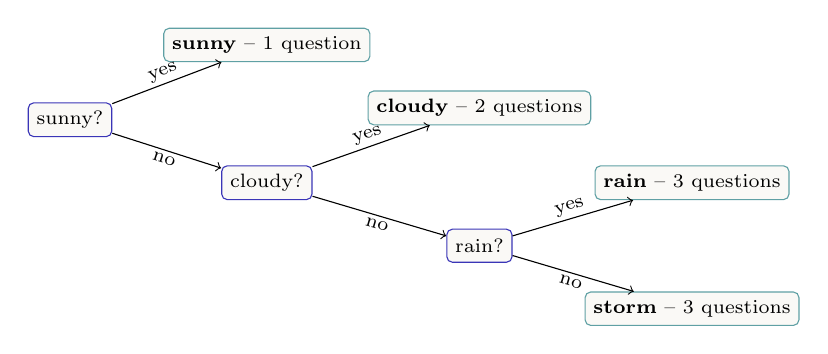
\begin{tikzpicture}[
  font=\scriptsize,
  q/.style={draw=RLBlue, fill=RLGray, rounded corners=2pt, inner sep=3pt,
            minimum height=4.2mm, align=center},
  leaf/.style={draw=RLGreen, fill=RLGray, rounded corners=2pt, inner sep=3pt,
               minimum height=4.2mm, align=center},
  lbl/.style={font=\scriptsize, inner sep=1.5pt}
]
  \node[q]    (q1) at (0,0)      {sunny?};
  \node[leaf] (l1) at (2.5,0.95) {\textbf{sunny} -- 1 question};
  \node[q]    (q2) at (2.5,-0.8) {cloudy?};
  \node[leaf] (l2) at (5.2,0.15) {\textbf{cloudy} -- 2 questions};
  \node[q]    (q3) at (5.2,-1.6) {rain?};
  \node[leaf] (l3) at (7.9,-0.8) {\textbf{rain} -- 3 questions};
  \node[leaf] (l4) at (7.9,-2.4) {\textbf{storm} -- 3 questions};
  \draw[->] (q1) -- node[lbl,above,sloped] {yes} (l1);
  \draw[->] (q1) -- node[lbl,below,sloped] {no}  (q2);
  \draw[->] (q2) -- node[lbl,above,sloped] {yes} (l2);
  \draw[->] (q2) -- node[lbl,below,sloped] {no}  (q3);
  \draw[->] (q3) -- node[lbl,above,sloped] {yes} (l3);
  \draw[->] (q3) -- node[lbl,below,sloped] {no}  (l4);
\end{tikzpicture}

\vspace{0.2em}
\raggedright
Average questions $= \tfrac12(1) + \tfrac14(2) + \tfrac18(3) + \tfrac18(3) = \mathbf{1.75}$. A rare outcome is expensive but seldom asked about; a common one is cheap and asked about often.
\end{frame}

\begin{frame}{Entropy}
\begin{rldefinition}
The \textbf{surprise} of an outcome is $\log_2 \tfrac{1}{p}$ -- how many yes/no questions it takes to pin down something of probability $p$. \emph{Weather:} sunny has $p = \tfrac12$, so $1$ bit; storm has $p = \tfrac18$, so $3$ bits.

\smallskip
The \textbf{entropy} $H(p)$ is the average surprise -- the average number of questions:
\[
H(p) \;=\; \sum_i p_i \log_2 \frac{1}{p_i} \;=\; -\sum_i p_i \log_2 p_i .
\]
\emph{Weather:} $H(p) = 1.75$ bits, exactly the tree's average.
\end{rldefinition}
\pause
\begin{itemize}
  \item \textbf{Certainty is free.} If one outcome has $p = 1$ the entropy is $0$: no questions needed.
  \item \textbf{Uniform is worst.} Four equally likely outcomes give $H = 2$ bits -- the most any four-outcome distribution can cost.
\end{itemize}
\end{frame}

\begin{frame}{Real Event: 360 Days of Weather in Bits}
\begin{columns}[T]
\column{0.50\textwidth}
\small
\begin{itemize}
  \item Each bar is one outcome's probability; the label above it is that outcome's surprise, $\log_2 \tfrac1p$.
  \pause
  \item \textbf{Entropy is the average of those labels}, weighted by the bars: $1.75$ bits.
  \pause
  \item Had the four outcomes been equally likely, every label would read $2$ bits and the average would be $2$. \textbf{Knowing the climate is worth $0.25$ bits a day} -- $90$ bits over those $360$ days.
  \pause
  \item \textbf{Read it:} entropy is low when probability is concentrated and high when it is spread out. It is the categorical answer to the question variance answers for numbers.
\end{itemize}
\column{0.48\textwidth}
\centering
\includegraphics[width=\linewidth]{figures/information_theory/info_entropy_weather.pdf}
\end{columns}
\end{frame}

\begin{frame}{When Is a Forecast Most Uncertain?}
\begin{columns}[T]
\column{0.50\textwidth}
\small
\begin{itemize}
  \item Take the simplest case -- rain or no rain -- and plot $H$ against the forecast probability.
  \pause
  \item \textbf{The peak is at $p = 0.5$}, where $H = 1$ bit: a fair coin is the most uncertain binary thing there is, and one question is always needed.
  \pause
  \item \textbf{Confidence is cheap either way.} A forecast of $0.11$ costs $0.50$ bits, and so does a forecast of $0.89$. Being sure it \emph{will} rain is as informative as being sure it will not.
  \pause
  \item \textbf{The curve is steep at the ends.} Moving a forecast from $0.5$ to $0.4$ buys almost nothing; moving it from $0.1$ to $0.01$ buys a lot.
\end{itemize}
\column{0.48\textwidth}
\centering
\includegraphics[width=\linewidth]{figures/information_theory/info_binary_entropy.pdf}
\end{columns}
\end{frame}

% ─── Cross-entropy ──────────────────────────────────────────────────────────
\begin{frame}{Why Do We Need Cross-Entropy?}
\begin{itemize}
  \item \textbf{The catch:} that question tree was built from the \emph{true} climate. Nobody hands you the true climate -- a forecaster has a belief $q$ and reality follows $p$.
  \pause
  \item \textbf{Everyday version:} a forecaster who thinks all four outcomes are equally likely will ask questions as if each cost $2$ bits. Reality still delivers sunny half the time, so he pays $2$ bits on a day that only needed $1$.
  \pause
  \item \textbf{The bill is a mixture:} how often each outcome \emph{actually} happens is set by $p$; how many questions each one \emph{costs him} is set by $q$.
  \pause
  \item \textbf{Cross-entropy} is that bill -- and it is the quantity you already minimise when you train a classifier.
\end{itemize}
\end{frame}

\begin{frame}{Cross-Entropy}
\begin{rldefinition}
The \textbf{cross-entropy} $H(p, q)$ is what you pay describing outcomes drawn from $p$ with a scheme built for $q$ -- \emph{real} frequencies, \emph{wrong} question tree:
\[
H(p, q) \;=\; -\sum_i p_i \log_2 q_i .
\]
\emph{Weather:} a forecaster who believes all four outcomes equally likely pays $2.00$ bits a day where the truth costs $1.75$.
\end{rldefinition}
\pause
\begin{itemize}
  \item \textbf{Never a bargain:} $H(p,q) \ge H(p)$, with equality only when $q = p$ -- the truth is its own cheapest scheme.
  \pause
  \item \textbf{And you have met it already,} under another name.
\end{itemize}
\end{frame}

\begin{frame}{Same Formula, Different Story}
\begin{itemize}
  \item Lecture 5 derived categorical cross-entropy as a negative log-likelihood: $-\sum_c y_c \log p_c$, with $y$ the one-hot label and $p$ the model's softmax.
  \pause
  \item \textbf{That is $H(y, p)$.} The one-hot label is a distribution putting all its mass on the true class, and the softmax is the belief being scored against it. Identical formula, no rearranging.
  \pause
  \item \textbf{Two readings of one number.} Lecture 5: \emph{how improbable was the data under my model?} Lecture 7: \emph{how many extra bits did my belief cost me?} Minimising either minimises the other.
  \pause
  \item \textbf{Bits or nats?} Frameworks use $\log_e$, so the unit is the \emph{nat} rather than the bit. It is a fixed factor of $\log 2 \approx 0.693$ and changes no decision -- our weather's $1.75$ bits is $1.21$ nats.
\end{itemize}
\end{frame}

\begin{frame}{Real Event: Three Forecasters, One Town}
\begin{columns}[T]
\column{0.50\textwidth}
\small
\begin{itemize}
  \item Three forecasters, the same town, the same $360$ days. The blue base is $H(p) = 1.75$; the coloured cap is what each one wastes.
  \pause
  \item \textbf{Knows the climate:} $1.75$ bits. Nothing wasted -- and still not zero.
  \pause
  \item \textbf{Assumes all four equal:} $2.00$ bits, wasting $0.25$ a day.
  \pause
  \item \textbf{Always says sunny} ($q = 0.90$ for sun): $2.57$ bits, wasting $0.82$. Confidence that is wrong is punished hardest -- $\log_2 \tfrac{1}{0.01}$ is $6.6$ bits on the day the storm arrives.
\end{itemize}
\column{0.48\textwidth}
\centering
\includegraphics[width=\linewidth]{figures/information_theory/info_cross_entropy_forecasters.pdf}
\end{columns}
\end{frame}

\begin{frame}{Why This Matters: The Loss You Cannot Get Below}
\begin{itemize}
  \item Every bar in that figure sat on the same blue base. \textbf{$H(p)$ is a floor} -- the part of the bill that comes from the world being uncertain, not from your model being wrong.
  \pause
  \item \textbf{So a cross-entropy loss of zero is not the target.} If two images with identical pixels genuinely carry different labels $70$/$30$ of the time, the best possible model still pays $H(0.7) = 0.88$ bits of loss on them. A model reporting near-zero training loss on noisy labels has memorised, not learned.
  \pause
  \item \textbf{Repeat this one:} \emph{cross-entropy splits into what the world does not know} ($H(p)$, unavoidable) \emph{plus what your model gets wrong} (the coloured cap). Only the second part is yours to reduce.
  \pause
  \item That second part has a name and a formula of its own -- the KL divergence, which opens Part 1.
\end{itemize}
\end{frame}

% \section{Lecture 7, Part 1: KL Divergence \& Mutual Information}

\begin{frame}
\vfill
\centering
{\color{RLBlue}\large Lecture 7}

\vspace{0.3em}
{\color{RLBlue}\Large\bfseries Part 1}

\vspace{0.6em}
{\Large KL Divergence \& Mutual Information}
\vfill
\end{frame}

\begin{frame}{Learning Goals}
\begin{itemize}
  \item Compute a KL divergence and read it as the avoidable part of a cross-entropy.
  \pause
  \item Explain why KL is not a distance, and what goes wrong if you treat it as one.
  \pause
  \item Use mutual information to say how much one answer tells you about another -- and recognise it as the criterion a decision tree splits on.
\end{itemize}
\end{frame}

% ─── KL divergence ──────────────────────────────────────────────────────────
\begin{frame}{Why Do We Need KL Divergence?}
\begin{itemize}
  \item \textbf{Why:} Part 0 ended with cross-entropy splitting into a floor you cannot move and a penalty you can. We want a name and a number for the second part alone.
  \pause
  \item \textbf{Everyday version:} the uniform forecaster paid $2.00$ bits a day where the truth cost $1.75$. The $1.75$ was the weather's fault. The extra $0.25$ was \emph{his}.
  \pause
  \item Subtracting the floor leaves a pure measure of \emph{how wrong the belief is}, with the world's own uncertainty removed. That is the KL divergence.
  \pause
  \item It answers questions the raw loss cannot: has my model moved closer to the truth, how far did this evidence shift my belief, and how far has a fine-tuned model drifted from the one it started as.
\end{itemize}
\end{frame}

\begin{frame}{KL Divergence}
\begin{rldefinition}
The \textbf{Kullback--Leibler divergence} $D_{\mathrm{KL}}(p \,\|\, q)$ is the cross-entropy minus the floor -- the extra cost of believing $q$ when the truth is $p$:
\[
D_{\mathrm{KL}}(p \,\|\, q) \;=\; H(p,q) - H(p) \;=\; \sum_i p_i \log_2 \frac{p_i}{q_i} .
\]
\emph{Weather:} the uniform forecaster has $2.00 - 1.75 = 0.25$ bits; the always-sunny one has $2.57 - 1.75 = 0.82$ bits.
\end{rldefinition}
\pause
\begin{itemize}
  \item \textbf{It is zero only for a perfect belief.} $D_{\mathrm{KL}} \ge 0$ always, and $= 0$ exactly when $q = p$ -- which is another way of saying the truth is its own cheapest description.
  \pause
  \item \textbf{Minimising cross-entropy is minimising KL.} They differ by $H(p)$, which does not depend on the model at all, so the two have the same minimiser.
\end{itemize}
\end{frame}

\begin{frame}{Real Event: How Much Did 100 Mornings Tell You?}
\begin{columns}[T]
\column{0.50\textwidth}
\small
\begin{itemize}
  \item Lecture 6's $7{:}40$ bus: prior Beta$(8,2)$, one morning at a time, plotting $D_{\mathrm{KL}}(\text{posterior} \,\|\, \text{prior})$.
  \pause
  \item \textbf{This is learning, measured.} At zero mornings the posterior \emph{is} the prior and the KL is exactly $0$. After $10$ mornings it is $0.66$ bits; after $100$, $1.76$.
  \pause
  \item \textbf{The jaggedness is real:} a late bus after a run of on-time ones pushes the posterior back toward the prior.
  \pause
  \item \textbf{Read it:} the prior was worth $10$ mornings, so the first ten roughly doubled what you knew -- the next $1.1$ bits took ninety more.
\end{itemize}
\column{0.48\textwidth}
\centering
\includegraphics[width=\linewidth]{figures/information_theory/info_kl_learning.pdf}
\end{columns}
\end{frame}

\begin{frame}{Why KL Is Not a Distance}
\begin{itemize}
  \item A distance is symmetric: the gap from A to B equals the gap from B to A. \textbf{KL is not.}
  \pause
  \item \textbf{The same two weather beliefs, swapped:} with $p$ the true climate and $q$ the always-sunny forecaster,
  \[
    D_{\mathrm{KL}}(p \,\|\, q) = 0.82 \text{ bits}, \qquad
    D_{\mathrm{KL}}(q \,\|\, p) = 0.54 \text{ bits}.
  \]
  \pause
  \item \textbf{Why the order matters:} $D_{\mathrm{KL}}(p \| q)$ averages over outcomes that \emph{really happen}, so it punishes $q$ for calling a real storm nearly impossible. Reverse it and those days barely count.
  \pause
  \item \textbf{The practical consequence:} minimising $D_{\mathrm{KL}}(p \| q)$ forces $q$ to put mass wherever the truth has any, giving a cautious, spread-out fit. Minimising $D_{\mathrm{KL}}(q \| p)$ lets $q$ pick one peak and ignore the rest. Two different answers from the same two distributions.
\end{itemize}
\end{frame}

\begin{frame}{Why This Matters: KL Is the Leash}
\begin{itemize}
  \item \textbf{Keeping a tuned model near its starting point.} Instruction tuning and RLHF add a KL penalty between the tuned model and the base model, so chasing a reward cannot pull the model into gibberish. The strength of that penalty is a dial you set (Module 5).
  \pause
  \item \textbf{Knowledge distillation.} A small model is trained to match a large one's full output distribution, not just its top answer. The objective is the KL between them -- which is why distillation transfers more than labels alone (Module 6, Lecture 2).
  \pause
  \item \textbf{Variational autoencoders.} The ELBO is a reconstruction term minus a KL between the encoder's distribution and a standard Gaussian prior -- the term that stops the latent space from scattering (Module 2).
  \pause
  \item \textbf{Repeat this one:} \emph{a KL term in a loss is always a leash -- it says ``fit the data, but do not wander far from this reference distribution''.}
\end{itemize}
\end{frame}

% ─── Mutual information ─────────────────────────────────────────────────────
\begin{frame}{Why Do We Need Mutual Information?}
\begin{itemize}
  \item \textbf{Why:} entropy scores one uncertain thing. Most questions involve two -- and what we want to know is whether looking at one \emph{reduces} our uncertainty about the other.
  \pause
  \item \textbf{Everyday version:} you want to know whether it will rain today. Glancing at the sky at $7$am tells you something. Checking whether today's date is even tells you nothing. Both are ``information'' in loose talk; only one of them is.
  \pause
  \item Lecture 2 defined independence as $P(A \cap B) = P(A)P(B)$ -- a yes/no verdict. Here we want the \emph{amount}: not ``are these related?'' but ``by how much?''
  \pause
  \item \textbf{The recipe:} measure your uncertainty about rain before looking, measure what is left after, and subtract.
\end{itemize}
\end{frame}

\begin{frame}{Mutual Information}
\begin{rldefinition}
The \textbf{conditional entropy} $H(Y \mid X)$ is how uncertain $Y$ still is once $X$ is known: the entropy of $Y$ within each answer, averaged over answers. The \textbf{mutual information} is the drop:
\[
I(X; Y) \;=\; H(Y) - H(Y \mid X) .
\]
\emph{Weather:} rain-or-storm has $H(Y) = 0.81$ bits; a grey sky at $7$am leaves $0.60$, so $I = 0.21$ bits.
\end{rldefinition}
\pause
\begin{itemize}
  \item \textbf{Never negative}, and exactly $0$ when $X$ and $Y$ are independent -- the quantitative version of Lecture 2's test.
  \pause
  \item \textbf{Symmetric}, unlike KL: what the sky says about rain equals what rain says about the sky.
\end{itemize}
\end{frame}

\begin{frame}{Real Event: Which Morning Question Should You Ask?}
\begin{columns}[T]
\column{0.50\textwidth}
\small
\begin{itemize}
  \item You may check one thing before leaving. The dashed line is $H(\text{wet}) = 0.81$ bits -- all there is to learn.
  \pause
  \item \textbf{Grey sky: $0.212$ bits.} It moves $P(\text{wet})$ from $0.25$ to $0.57$ when grey, and to $0.08$ when clear.
  \pause
  \item \textbf{Wind from the west: $0.022$ bits.} Related, but it only shifts $P(\text{wet})$ to $0.33$. A tenth as useful.
  \pause
  \item \textbf{Even-numbered date: exactly $0$} -- independent of the weather. \textbf{That ranking is feature selection}: how many bits does each candidate input actually buy?
\end{itemize}
\column{0.48\textwidth}
\centering
\includegraphics[width=\linewidth]{figures/information_theory/info_information_gain.pdf}
\end{columns}
\end{frame}

\begin{frame}{Why This Matters: Information Gain \emph{Is} Mutual Information}
\begin{itemize}
  \item A decision tree, at every node, asks: which question should I split on? It scores each candidate by \textbf{information gain} -- the entropy before the split, minus the average entropy of the two branches.
  \pause
  \item \textbf{That is the formula on the previous slide, unchanged.} $H(Y) - H(Y \mid X)$. The tree in Module 1, Lecture 5 is running exactly the calculation that ranked ``grey sky'' above ``wind'' above ``even date''.
  \pause
  \item So the guessing game from Part 0 was not an analogy. \textbf{A decision tree is twenty questions, played greedily}, and entropy is what tells it which question to ask next.
  \pause
  \item \textbf{Elsewhere in AI:} mutual information scores which features to keep before training, and contrastive objectives like InfoNCE maximise a bound on the mutual information between two views of the same thing -- which is how modern representations are learned without labels (Modules 2 and 3).
\end{itemize}
\end{frame}

\begin{frame}{Where This Goes Next}
\begin{itemize}
  \item \textbf{Lecture 8 -- the exponential family:} entropy reappears as the quantity a distribution maximises subject to what you know. The Gaussian, the Bernoulli and the Poisson all fall out of that single principle.
  \pause
  \item \textbf{Lecture 10 -- model evaluation:} a model's average negative log-likelihood on held-out data is its cross-entropy against reality, which is what perplexity reports.
  \pause
  \item \textbf{Module 1, Lecture 5 -- decision trees:} information gain, exactly as defined here.
  \pause
  \item \textbf{Modules 2, 5 and 6:} the KL term in a VAE, the KL leash in RLHF, and the KL objective in distillation -- one quantity, three places.
\end{itemize}
\end{frame}

\begin{frame}{Summary}
\begin{itemize}
  \item \textbf{Entropy} $H(p) = -\sum p_i \log_2 p_i$ is the average number of yes/no questions needed to pin down an outcome. It is $0$ for certainty and largest for a uniform distribution.
  \pause
  \item \textbf{Cross-entropy} $H(p,q) = -\sum p_i \log_2 q_i$ is what you pay using belief $q$ when reality is $p$. It is never below $H(p)$, and with $p$ a one-hot label it is the loss from Lecture 5.
  \pause
  \item \textbf{KL divergence} is the difference, $H(p,q) - H(p)$: the avoidable part. Zero only when $q = p$, never negative, and \emph{not} symmetric.
  \pause
  \item \textbf{Mutual information} $I(X;Y) = H(Y) - H(Y \mid X)$ is how many bits $X$ buys you about $Y$. Zero exactly when they are independent.
  \pause
  \item \textbf{One sentence to keep:} \emph{your loss is a cross-entropy, its floor is the world's own uncertainty, and everything above that floor is a KL divergence you can still remove.}
\end{itemize}
\end{frame}


% \section{Lecture 8, Part 0: The Exponential Family}

\begin{frame}
\vfill
\centering
{\color{RLBlue}\large Lecture 8}

\vspace{0.3em}
{\color{RLBlue}\Large\bfseries Part 0}

\vspace{0.6em}
{\Large The Exponential Family}
\vfill
\end{frame}

\begin{frame}{Learning Goals}
\begin{itemize}
  \item Rewrite a Bernoulli and a Categorical by hand, and recognize the logit and the softmax as what falls out.
  \pause
  \item Read the three pieces $\eta$, $T(x)$ and $A(\eta)$ off a distribution you already know.
  \pause
  \item Use $A'(\eta) = E[T(X)]$ to turn maximum likelihood into ``match the averages''.
\end{itemize}
\end{frame}

% ─── Motivation ─────────────────────────────────────────────────────────────
\begin{frame}{Why Do So Many Distributions Look Alike?}
\begin{itemize}
  \item \textbf{Why:} the two derivations in Lecture 5 came out suspiciously similar. Bernoulli: $\hat{p} = k/n$. Gaussian: $\hat{\mu} = \bar{x}$. Both answers were \emph{the average of something} -- and fitting a Poisson would have given $\hat{\lambda} = \bar{k}$, the average once more.
  \pause
  \item Lecture 6 had the same experience from the other side: every conjugate update turned out to be \emph{add counts to the prior}.
  \pause
  \item And the softmax has now appeared twice -- once as a Categorical in Lecture 3, once inside cross-entropy in Lecture 5 -- without anyone saying where it comes from.
  \pause
  \item \textbf{Those are not three coincidences.} Bernoulli, Poisson, Gaussian, Categorical, Beta and Dirichlet are all one family wearing different clothes. This lecture undresses them.
\end{itemize}
\end{frame}

% ─── Bernoulli rewrite: eta appears ─────────────────────────────────────────
\begin{frame}{Worked Example: Rewriting the Bernoulli}
\small
Take the Bernoulli of Lecture 3, written for $x \in \{0,1\}$, and do nothing but algebra:
\[
p^{x}(1-p)^{1-x}
\;=\; \exp\big( x\log p + (1-x)\log(1-p) \big)
\;=\; \exp\Big( x\,\underbrace{\log\tfrac{p}{1-p}}_{\textstyle \eta} \;+\; \log(1-p) \Big).
\]
\pause
\begin{itemize}
  \item \textbf{Nothing was assumed.} We took a logarithm and collected the terms in $x$ -- and one particular combination of $p$ \emph{appeared} on its own: $\eta = \log\frac{p}{1-p}$.
  \pause
  \item That combination already has a name: the \textbf{logit}. It is the number a classifier's final layer produces, \emph{before} any sigmoid is applied.
  \pause
  \item \textbf{Coffee shop:} $p = 0.3$ gives $\eta = \log\frac{0.3}{0.7} = -0.85$. Negative because pastries are the minority outcome, and $\eta = 0$ would mean $p = 0.5$.
\end{itemize}
\end{frame}

\begin{frame}{From Probability to Logit and Back}
\begin{columns}[T]
\column{0.50\textwidth}
\small
\begin{itemize}
  \item \textbf{Top:} $\eta = \log\frac{p}{1-p}$ stretches the interval $(0,1)$ out over the whole line. Certainty at either end runs off to $\pm\infty$.
  \pause
  \item \textbf{Bottom:} the inverse squashes it back, $p = \sigma(\eta) = \frac{1}{1+e^{-\eta}}$ -- the sigmoid.
  \pause
  \item \textbf{Why a network works in $\eta$:} a layer outputs any real number it likes. Probabilities would have to be kept inside $[0,1]$ by force; logits need no policing.
  \pause
  \item The orange dot is the same coffee shop on both panels: $p = 0.3 \leftrightarrow \eta = -0.85$.
\end{itemize}
\column{0.48\textwidth}
\centering
\includegraphics[width=0.96\linewidth]{figures/expfamily/expfamily_logit_map.pdf}
\end{columns}
\end{frame}

% ─── Categorical rewrite: softmax appears ───────────────────────────────────
\begin{frame}{Worked Example: Rewriting the Categorical}
\small
Write the cup size as a one-hot vector $x = (x_1, \dots, x_k)$ with exactly one entry equal to $1$:
\[
\prod_{c=1}^{k} p_c^{\,x_c}
\;=\; \exp\Big( \sum_{c=1}^{k} x_c \log p_c \Big),
\qquad \eta_c = \log p_c .
\]
\pause
\begin{itemize}
  \item Since $\sum_c e^{\eta_c} = \sum_c p_c = 1$, we may subtract $A(\eta) = \log\sum_c e^{\eta_c} = 0$ without changing anything -- and \emph{now} adding the same constant to every $\eta_c$ is harmless, because $A$ absorbs it.
  \pause
  \item So the $\eta_c$ are unnormalized \textbf{scores}, not log-probabilities. Inverting the map to recover the shares:
  \[
    p_c = \frac{e^{\eta_c}}{\sum_{j} e^{\eta_j}} .
  \]
  \pause
  \item \textbf{That is the softmax} -- derived, not introduced. \emph{Coffee shop:} scores $(-1.61, -0.69, -1.20)$ return exactly $(0.2,\, 0.5,\, 0.3)$, and so do those three scores plus $2$.
\end{itemize}
\end{frame}

% ─── The general form, now earned ───────────────────────────────────────────
\begin{frame}{The Exponential Family}
\begin{rldefinition}
A distribution is in the \textbf{exponential family} if it can be written
\[
p(x \mid \eta) = h(x)\,\exp\big( \eta^{\top} T(x) - A(\eta) \big) .
\]
\textbf{$T(x)$ -- the sufficient statistic:} the only thing the data gets to say. \emph{Bernoulli:} $T(x)=x$.\\
\textbf{$\eta$ -- the natural parameter:} the coordinate the family is straight in. \emph{Bernoulli:} the logit.\\
\textbf{$A(\eta)$ -- the log-partition function:} whatever it takes to make the total $1$. \emph{Bernoulli:} $\log(1+e^{\eta})$.\\
\textbf{$h(x)$ -- the base measure:} the leftover bookkeeping that never involves $\eta$. \emph{Bernoulli:} $1$.
\end{rldefinition}
\pause
\begin{itemize}
  \item The shape is the whole content: $x$ and $\eta$ meet \emph{only} in the product $\eta^{\top}T(x)$. Everything that follows in this lecture is a consequence of that one restriction.
\end{itemize}
\end{frame}

\begin{frame}{One Form, Four Distributions}
\footnotesize
\centering
\begin{tabular}{l|ccc}
Distribution & $T(x)$ & $\eta$ & $A(\eta)$ \\
\hline
Bernoulli$(p)$ & $x$ & $\log\frac{p}{1-p}$ & $\log(1+e^{\eta})$ \\[2pt]
Poisson$(\lambda)$ & $k$ & $\log \lambda$ & $e^{\eta}$ \\[2pt]
Gaussian$(\mu,\sigma^2)$, $\sigma$ known & $x$ & $\mu/\sigma^{2}$ & $\sigma^{2}\eta^{2}/2$ \\[2pt]
Categorical$(p_1,\dots,p_k)$ & one-hot $x$ & scores $\eta_c$ & $\log\sum_c e^{\eta_c}$ \\
\end{tabular}

\vspace{0.6em}
\raggedright
\begin{itemize}
  \item \textbf{The Beta and the Dirichlet are in it too}, with the roles swapped: there the \emph{probability} is the data, and $T(p) = (\log p, \log(1-p))$ with $\eta = (\alpha-1, \beta-1)$.
  \pause
  \item \textbf{Not everything is.} A Student-$t$ or a mixture of two Gaussians cannot be squeezed into this form -- which is exactly why they are harder to fit.
\end{itemize}
\end{frame}

% ─── A(eta) ─────────────────────────────────────────────────────────────────
\begin{frame}{Why Do We Need $A(\eta)$?}
\begin{itemize}
  \item \textbf{Why:} $h(x)e^{\eta^{\top}T(x)}$ is a perfectly good \emph{shape}, but its total is not $1$. $A(\eta)$ is the log of that total, subtracted off to fix it:
  \[
    A(\eta) = \log \sum_{x} h(x)\,e^{\eta^{\top}T(x)} .
  \]
  \pause
  \item \textbf{Numerical example, Bernoulli:} the two unnormalized weights are $e^{0}=1$ and $e^{\eta}$, so $A(\eta)=\log(1+e^{\eta})$. At $\eta = -0.85$ that is $\log(1.429) = 0.357$, which is exactly $-\log(1-p) = -\log 0.7$.
  \pause
  \item \textbf{For the Categorical it is the log-sum-exp}, $\log\sum_c e^{\eta_c}$ -- the same expression every deep learning framework computes to normalize a softmax.
  \pause
  \item So $A$ looks like bookkeeping. The next slide shows it is nothing of the kind.
\end{itemize}
\end{frame}

\begin{frame}{The Slope of $A$ Is the Mean}
\begin{columns}[T]
\column{0.50\textwidth}
\small
\begin{itemize}
  \item Differentiate $A$ once for the mean of $T$, twice for its variance:
  \[
    A'(\eta) = E_{\eta}[T], \qquad A''(\eta) = \mathrm{Var}_{\eta}(T).
  \]
  \pause
  \item \textbf{Bernoulli:} $A' = \sigma(\eta) = 0.30 = p$ at $\eta = -0.85$, and $A'' = p(1-p) = 0.21$ -- Lecture 3's variance.
  \pause
  \item \textbf{Poisson:} $A = e^{\eta}$, so $A' = A'' = \lambda$. \emph{That} is why its mean equals its variance -- the exponential is its own derivative.
\end{itemize}
\column{0.48\textwidth}
\centering
\includegraphics[width=0.96\linewidth]{figures/expfamily/expfamily_log_partition.pdf}
\end{columns}
\end{frame}

% ─── AI payoff 1 ────────────────────────────────────────────────────────────
\begin{frame}{Why This Matters: The Last Layer of a Classifier}
\begin{itemize}
  \item A classification network ends by producing $k$ raw numbers and pushing them through a softmax. Those raw numbers are called logits, and the name is not an analogy: \textbf{they are the natural parameters $\eta$ of a Categorical.}
  \pause
  \item \textbf{So the last layer of a classifier is an exponential-family parameterization}, and the sigmoid and the softmax are not design choices -- they are the inverse map back from $\eta$ to probabilities.
  \pause
  \item That also explains a practical detail: frameworks pair \texttt{logits} with the loss in one function rather than applying softmax first, because $\log\sum_c e^{\eta_c}$ is $A(\eta)$ and it is more stable computed once.
  \pause
  \item \textbf{Repeat this one:} \emph{a network predicts $\eta$; the link function converts it to a distribution.} That sentence is also the definition of a generalized linear model.
\end{itemize}
\end{frame}

% ─── MLE as moment matching ─────────────────────────────────────────────────
\begin{frame}{Worked Example: MLE Is Moment Matching}
\small
For $n$ independent draws the log-likelihood is a sum, and the exponential form collapses it:
\[
\ell(\eta) = \eta^{\top}\sum_{i=1}^{n} T(x_i) \;-\; n\,A(\eta) + \text{const},
\qquad
\frac{\partial \ell}{\partial \eta} = \sum_{i=1}^{n} T(x_i) \;-\; n\,A'(\eta).
\]
\pause
\begin{itemize}
  \item Set the derivative to zero and divide by $n$. Using $A'(\eta) = E_{\eta}[T]$:
  \[
    \boxed{\; E_{\hat{\eta}}[T(X)] \;=\; \frac{1}{n}\sum_{i=1}^{n} T(x_i) \;}
  \]
  \pause
  \item \textbf{In words:} pick the parameter whose predicted average matches the observed one. That is the whole of maximum likelihood for this family.
  \pause
  \item \textbf{Both of Lecture 5's results, and the Poisson for free:} $\sigma(\hat{\eta}) = \bar{x}$ gives $\hat{p} = k/n$; $\sigma^{2}\hat{\eta} = \bar{x}$ gives $\hat{\mu} = \bar{x}$; $e^{\hat{\eta}} = \bar{k}$ gives $\hat{\lambda} = \bar{k}$.
\end{itemize}
\end{frame}

\begin{frame}{Why This Matters: Fitting Means Matching Averages}
\begin{columns}[T]
\column{0.50\textwidth}
\small
\begin{itemize}
  \item The boxed equation, drawn twice: slide the red line -- the data's average -- and read off where it meets the model's mean curve.
  \pause
  \item \textbf{Bernoulli:} $66$ of $200$ orders, so the line sits at $0.33$ and $\hat{\eta} = -0.71$.
  \pause
  \item \textbf{Poisson:} $3.96$ arrivals per ten minutes, so $\hat{\eta} = \log 3.96 = 1.38$.
  \pause
  \item \textbf{In AI:} the gradient is \emph{observed} $T$ minus \emph{expected} $T$ -- the training signal for log-linear and energy-based models, and the reason they need some way to estimate $E_{\eta}[T]$.
\end{itemize}
\column{0.48\textwidth}
\centering
\includegraphics[width=0.96\linewidth]{figures/expfamily/expfamily_moment_matching.pdf}
\end{columns}
\end{frame}

% \section{Lecture 8, Part 1: Sufficient Statistics}

\begin{frame}
\vfill
\centering
{\color{RLBlue}\large Lecture 8}

\vspace{0.3em}
{\color{RLBlue}\Large\bfseries Part 1}

\vspace{0.6em}
{\Large Sufficient Statistics}
\vfill
\end{frame}

\begin{frame}{Learning Goals}
\begin{itemize}
  \item Say what a sufficient statistic is, and check a candidate with the factorization test.
  \pause
  \item Explain why conjugate updating in Lecture 6 was always ``add counts''.
  \pause
  \item Name what you may throw away from a dataset without losing anything about $\theta$ -- and what you may not.
\end{itemize}
\end{frame}

% ─── Motivation ─────────────────────────────────────────────────────────────
\begin{frame}{Why Do We Need Sufficient Statistics?}
\begin{itemize}
  \item \textbf{Why:} Lecture 5 fitted $p$ from $200$ coffee orders and the answer was $\hat{p} = 66/200$. Two hundred records went in; \emph{one number} came out.
  \pause
  \item \textbf{The uncomfortable question:} we still hold those $200$ records -- who bought what, in which order, on which morning. Did throwing all of that away cost us anything about $p$?
  \pause
  \item \textbf{The answer is no, and it is exact, not approximate.} Any two records with the same total of $66$ give the same likelihood curve, hence the same estimate, the same interval, and the same posterior.
  \pause
  \item So $66$ is not a summary of the data. For the question ``what is $p$?'' it \emph{is} the data.
\end{itemize}
\end{frame}

\begin{frame}{The Sufficient Statistic}
\begin{rldefinition}
A statistic $T$ is \textbf{sufficient} for $\theta$ when the data tells you nothing more about $\theta$ once you know $T$. Formally, $p(x \mid T(x), \theta)$ does not depend on $\theta$.

\smallskip
\textbf{Bernoulli:} the number of successes. \emph{$66$ pastry orders} -- the order they arrived in is irrelevant to $p$.\\
\textbf{Poisson:} the total count. \emph{Arrivals summed over all windows.}\\
\textbf{Gaussian:} the two sums $\sum x_i$ and $\sum x_i^{2}$ -- enough to recover $\bar{x}$ and $\hat{\sigma}^2$.
\end{rldefinition}
\pause
\begin{itemize}
  \item \textbf{Part 0 already proved it for the whole family.} The log-likelihood was $\eta^{\top}\sum_i T(x_i) - nA(\eta)$: the data reaches $\eta$ \emph{only} through $\sum_i T(x_i)$. Nothing else can matter, because nothing else is there.
\end{itemize}
\end{frame}

\begin{frame}{Three Records, One Likelihood Curve}
\begin{columns}[T]
\column{0.50\textwidth}
\small
\begin{itemize}
  \item Three ten-morning records, $20$ orders a morning: steady, one sell-out day, or slowly building. All total $66$ of $200$.
  \pause
  \item \textbf{The lower panel plots all three log-likelihoods.} You see one curve because they \emph{are} one curve: $\ell(p) = 66\log p + 134\log(1-p)$.
  \pause
  \item Same peak, same curvature. The shape of the record was never in the answer.
\end{itemize}
\column{0.48\textwidth}
\centering
\includegraphics[width=0.96\linewidth]{figures/expfamily/expfamily_sufficiency.pdf}
\end{columns}
\end{frame}

% ─── Fisher-Neyman ──────────────────────────────────────────────────────────
\begin{frame}{The Factorization Test}
\begin{rldefinition}
\textbf{Fisher--Neyman factorization.} $T$ is sufficient for $\theta$ exactly when the density splits into two pieces --
\[
p(x \mid \theta) = \underbrace{g\big(T(x),\, \theta\big)}_{\text{touches } \theta \text{ only via } T} \;\times\; \underbrace{h(x)}_{\text{no } \theta \text{ at all}} .
\]
\emph{Reading it:} if you can push every appearance of $\theta$ into a factor that sees the data only through $T$, then $T$ carries all the information.
\end{rldefinition}
\pause
\begin{itemize}
  \item \textbf{This is why the exponential family has such tidy statistics.} Its definition \emph{is} the factorization: $h(x)$ is the second piece and $\exp(\eta^{\top}T(x) - A(\eta))$ is the first.
  \pause
  \item So membership in the family hands you the sufficient statistic for free -- just read off $T$.
\end{itemize}
\end{frame}

\begin{frame}{Worked Example: What a Gaussian Needs}
\begin{itemize}
  \item Lecture 5 measured $40$ espresso shots and reported $\hat{\mu} = 29.88$\,ml, $\hat{\sigma} = 1.27$\,ml. Expanding the square in the density:
  \[
    \prod_i e^{-\frac{(x_i-\mu)^2}{2\sigma^2}}
    = \exp\Big( -\tfrac{1}{2\sigma^2}\textstyle\sum_i x_i^{2} + \tfrac{\mu}{\sigma^{2}}\sum_i x_i - \tfrac{n\mu^{2}}{2\sigma^{2}} \Big).
  \]
  \pause
  \item The data appears \emph{only} as $\sum_i x_i$ and $\sum_i x_i^{2}$. Here that is $1195.2$ and $35777.1$.
  \pause
  \item \textbf{Two numbers replace forty measurements} -- and would replace forty thousand. The sufficient statistic does not grow with the sample.
  \pause
  \item \textbf{But be careful what you are sufficient \emph{for}.} Those two numbers fix $\hat{\mu}$ and $\hat{\sigma}$, and say nothing about whether the shots were normally distributed at all. Checking the \emph{model} needs the raw data back.
\end{itemize}
\end{frame}

% ─── The Lecture 6 promise ──────────────────────────────────────────────────
\begin{frame}{Why Conjugacy Worked}
\begin{itemize}
  \item Lecture 6 showed that updating a Beta or a Dirichlet was pure counting, and left the reason open. Here it is.
  \pause
  \item The posterior is prior times likelihood, and the likelihood is the exponential form:
  \[
    p(\eta \mid x_{1:n}) \;\propto\; p(\eta)\,\exp\Big( \eta^{\top}\textstyle\sum_i T(x_i) - n A(\eta) \Big).
  \]
  \pause
  \item \textbf{The data enters through exactly two numbers:} $\sum_i T(x_i)$ and $n$. A prior that already stores a pretend $\sum T$ and a pretend $n$ therefore updates by \emph{adding} to them -- and stays in its own family.
  \pause
  \item \textbf{So ``a prior is worth $n$ observations'' was literal.} Beta$(8,2)$ stores $8$ successes out of $10$; the $22$ on-time mornings simply add. Nothing was analogy.
\end{itemize}
\end{frame}

% ─── AI payoffs ─────────────────────────────────────────────────────────────
\begin{frame}{Why This Matters: A Counter Instead of a Dataset}
\begin{itemize}
  \item If $\sum_i T(x_i)$ and $n$ are all that any estimate can use, you never have to store the data. Keep the running totals, discard each record as it passes, and the answer is \emph{identical} to the one you would get from the whole archive.
  \pause
  \item \textbf{Streaming estimation:} a shop tracking its pastry rate keeps two integers, not a database. The same trick runs on a sensor with no disk.
  \pause
  \item \textbf{In AI:} batch normalization keeps a running mean and variance -- precisely the Gaussian sufficient statistics -- rather than replaying the training set.
  \pause
  \item \textbf{Federated learning} turns on the same fact: a device can send $\sum T$ and $n$ instead of the records themselves, and the server's estimate loses nothing.
  \pause
  \item \textbf{The limit is real, though.} Sufficiency is always \emph{for a model}. Change the question -- outliers, drift, a different family -- and yesterday's counters no longer answer it.
\end{itemize}
\end{frame}

\begin{frame}{Why an AI Course Teaches the Exponential Family}
\begin{itemize}
  \item \textbf{It explains the output layer.} Sigmoid and softmax are the inverse maps from $\eta$ back to probabilities, and ``logit'' is the natural parameter's real name.
  \pause
  \item \textbf{It explains the training signal.} Fitting is matching expected statistics to observed ones, so the gradient is \emph{observed} $T$ minus \emph{expected} $T$ -- the recipe behind log-linear and energy-based models.
  \pause
  \item \textbf{It is the definition of a generalized linear model.} Predict $\eta$ with a linear function of the inputs and map back: identity link gives linear regression, logit link gives logistic regression, log link gives Poisson regression. One recipe, three familiar methods.
  \pause
  \item \textbf{It is what makes variational inference tractable.} Restricting an approximate posterior to an exponential family is what turns its training objective into arithmetic you can differentiate (Module 2, Lecture 13).
\end{itemize}
\end{frame}

\begin{frame}{Where This Goes Next}
\begin{itemize}
  \item \textbf{Lecture 9 -- regression:} least squares is the Gaussian member with $\eta$ a linear function of the inputs -- the first generalized linear model.
  \pause
  \item \textbf{Back to Lecture 7:} the KL divergence between two members of one family has a closed form built entirely from $A$ -- no integration needed.
  \pause
  \item \textbf{Module 1, Lecture 13 -- logistic regression:} the Bernoulli member with $\eta = w^{\top}x$. Its loss, its link and its gradient are all on the previous slides.
  \pause
  \item \textbf{Module 2 -- variational autoencoders:} Gaussian encoders and exponential-family posteriors, for exactly the tractability reason above.
\end{itemize}
\end{frame}

\begin{frame}{Summary}
\begin{itemize}
  \item A distribution is in the \textbf{exponential family} if $p(x\mid\eta) = h(x)\exp(\eta^{\top}T(x) - A(\eta))$. Bernoulli, Poisson, Gaussian, Categorical, Beta and Dirichlet all are; a mixture is not.
  \pause
  \item The \textbf{natural parameter} of a Bernoulli is the logit, and the inverse map for a Categorical is the softmax -- so a classifier's last layer is this family in disguise.
  \pause
  \item $A'(\eta) = E[T(X)]$ and $A''(\eta) = \mathrm{Var}(T(X))$. That is why the Poisson's mean equals its variance, and it is where every mean in Lecture 5 came from.
  \pause
  \item \textbf{Maximum likelihood is moment matching:} pick $\hat\eta$ so the model's expected statistic equals the observed average. One line replaces three separate derivations.
  \pause
  \item A \textbf{sufficient statistic} is everything the data can say about $\theta$. It explains why conjugate updating was counting, and why a running total can replace an archive -- for that model, and no other.
\end{itemize}
\end{frame}


% \section{Lecture 9, Part 0: Correlation \& Regression}

\begin{frame}
\vfill
\centering
{\color{RLBlue}\large Lecture 9}

\vspace{0.3em}
{\color{RLBlue}\Large\bfseries Part 0}

\vspace{0.6em}
{\Large Correlation \& Regression}
\vfill
\end{frame}

\begin{frame}{Learning Goals}
\begin{itemize}
  \item Measure how two quantities move together with covariance, and make that measurement unit-free with the correlation $r$.
  \pause
  \item Fit a straight line by ordinary least squares, read its slope, and use its residuals to ask whether a line was the right shape.
  \pause
  \item Interpret $R^2$, and explain why fitting a line by least squares is maximum likelihood estimation in disguise.
\end{itemize}
\end{frame}

% ─── Covariance and correlation ─────────────────────────────────────────────
\begin{frame}{Why Do We Need Correlation?}
\begin{itemize}
  \item Everything so far described \emph{one} quantity at a time -- a mean, a spread, a distribution. But the useful questions are almost always about a \emph{pair}: do warm days sell more iced coffee, do extra study hours raise the mark, does a longer commute mean a later arrival?
  \pause
  \item Lecture 4 already produced the number for this. The covariance of temperature and iced coffees over $300$ trading days was $49.6$ -- positive, so they rise together.
  \pause
  \item \textbf{But $49.6$ what?} Its units are $^\circ$C$\,\cdot\,$cups. Record the temperature in Fahrenheit and the same relationship reports $89.3$ instead. A number whose size depends on the units cannot say whether a relationship is \emph{strong}.
  \pause
  \item So we need the covariance rescaled into something comparable across quantities. That is the correlation.
\end{itemize}
\end{frame}

\begin{frame}{Covariance and Correlation}
\begin{rldefinition}
\textbf{Covariance} -- the average product of the two deviations from their means: positive when the pair rises together, negative when one rises as the other falls.
\[
  s_{xy} = \frac{1}{n-1}\sum_{i=1}^{n}(x_i - \bar{x})(y_i - \bar{y}) = 49.6\ ^\circ\text{C}\cdot\text{cups}.
\]
\textbf{Correlation} -- that covariance divided by both standard deviations, which cancels the units and traps the answer in $[-1,1]$:
$r = s_{xy}/(s_x s_y) = 49.6/(5.65 \times 11.33) = 0.77$.
\end{rldefinition}
\pause
\begin{itemize}
  \item $r = +1$ is a perfect rising line, $r = -1$ a perfect falling one, $r = 0$ no \emph{straight-line} relationship. Here $0.77$ is strong and positive.
\end{itemize}
\end{frame}

\begin{frame}{Real Event: Hot Days and Iced Coffee}
\begin{columns}[T]
\column{0.50\textwidth}
\small
\begin{itemize}
  \item The grey crosshair marks the mean point $(21.8\,^\circ$C$,\ 39.5$ cups$)$ and cuts the plot into four quadrants.
  \pause
  \item \textbf{Why the covariance comes out positive:} a warm, busy day sits upper-right, where both deviations are positive, so their product is positive. A cold, quiet day sits lower-left, where both are negative -- and a negative times a negative is positive again.
  \pause
  \item Days in the other two quadrants contribute negative products. The covariance is just the average, so it is positive when the upper-right and lower-left days win.
\end{itemize}
\column{0.48\textwidth}
\centering
\includegraphics[width=\linewidth]{figures/regression/regression_scatter_corr.pdf}
\end{columns}
\end{frame}

% ─── Regression ─────────────────────────────────────────────────────────────
\begin{frame}{Why Do We Need a Line, Not Just a Number?}
\begin{itemize}
  \item $r = 0.77$ says the relationship is strong and positive. It does \emph{not} say how much.
  \pause
  \item The shop's actual question is: \emph{tomorrow is forecast $3^\circ$ warmer -- how many more cups should I prepare?} A correlation cannot answer that; it has no units left to answer it with.
  \pause
  \item A \textbf{line} can. Its slope is a rate -- cups per degree -- and it also predicts at temperatures we have never recorded.
  \pause
  \item Fitting that line is the smallest possible act of machine learning: choose parameters so the predictions miss the data as little as possible.
\end{itemize}
\end{frame}

\begin{frame}{Ordinary Least Squares}
\begin{rldefinition}
\textbf{Ordinary least squares} -- of all lines $\hat{y} = a + bx$, take the one whose vertical gaps to the data are smallest in total, measured by the sum of \emph{squared} gaps:
\[
  (a, b) = \arg\min_{a,b} \sum_{i=1}^{n}\big(y_i - a - b x_i\big)^2 .
\]
Minimising gives closed forms, not a search: $b = s_{xy}/s_x^2$ and $a = \bar{y} - b\,\bar{x}$.
\end{rldefinition}
\pause
\begin{itemize}
  \item That second formula says the line \textbf{always passes through the mean point} $(\bar{x}, \bar{y})$, so the slope alone fixes it.
  \pause
  \item \textbf{Why squared gaps?} They make the minimisation solvable in closed form and punish one big miss more than several small ones. Shortly, Lecture 5 supplies the real reason.
\end{itemize}
\end{frame}

\begin{frame}{Worked Example: Fitting the Line by Hand}
\begin{itemize}
  \item Everything needed is already in Lecture 4's covariance matrix: $s_x^2 = 31.9$, $s_{xy} = 49.6$, with $\bar{x} = 21.81\,^\circ$C and $\bar{y} = 39.49$ cups.
  \pause
  \item \textbf{Slope:} $b = \dfrac{s_{xy}}{s_x^2} = \dfrac{49.6}{31.9} = 1.5548$ cups per degree. \textbf{Intercept:} $a = \bar{y} - b\bar{x} = 39.49 - 1.5548(21.81) = 5.6$ cups, giving
  \[ \hat{y} = 5.6 + 1.55\,x \]
  \pause
  \item \textbf{Reading the slope:} each extra degree sells about $1.55$ more iced coffees, so a forecast $3^\circ$ warmer means roughly $5$ extra cups. That is the shop's answer.
  \pause
  \item \textbf{Predicting:} at $25^\circ$C, $\hat{y} = 5.6 + 1.55(25) = 44$ cups. The intercept $5.6$ is a formality -- it is sales at $0^\circ$C, far outside anything observed.
\end{itemize}
\end{frame}

\begin{frame}{Real Event: The Fitted Line and Its Residuals}
\begin{columns}[T]
\column{0.50\textwidth}
\small
\begin{itemize}
  \item A \textbf{residual} is what the line missed by: $e_i = y_i - \hat{y}_i$. The red segments are the twelve largest.
  \pause
  \item \textbf{Example:} one day reached $22.4^\circ$C and sold $28$ cups against a predicted $40.5$, so $e = 28 - 40.5 = -12.5$. Least squares forces the residuals to average exactly zero, so only their size matters: here $7.2$ cups.
  \pause
  \item \textbf{The lower panel is the real test.} Residuals against temperature show no leftover pattern -- no curve, no fanning -- so a line was the right shape. An arc there would mean real structure was missed.
\end{itemize}
\column{0.48\textwidth}
\centering
\includegraphics[width=\linewidth]{figures/regression/regression_fit_residuals.pdf}
\end{columns}
\end{frame}

% ─── R-squared ──────────────────────────────────────────────────────────────
\begin{frame}{Why Do We Need $R^2$?}
\begin{columns}[T]
\column{0.50\textwidth}
\small
\begin{rldefinition}
\footnotesize
$R^2$ -- the share of the outcome's variation the line accounts for: compare the gaps to a flat line at $\bar{y}$ with the gaps to the fitted line.
\[
  R^2 = 1 - \frac{\mathrm{SS}_{\text{res}}}{\mathrm{SS}_{\text{tot}}}
      = 1 - \frac{15{,}348}{38{,}385} = 0.60 .
\]
\end{rldefinition}
\pause
\begin{itemize}
  \item Knowing the temperature removes $60\%$ of the guesswork about the day's sales.
  \pause
  \item With one predictor, $R^2$ is exactly $r^2$ -- to full precision $r = 0.7747$, and $0.7747^2 = 0.60$.
\end{itemize}
\column{0.48\textwidth}
\centering
\includegraphics[width=\linewidth]{figures/regression/regression_r_squared.pdf}
\end{columns}
\end{frame}

\begin{frame}{Why This Matters: Least Squares \emph{Is} Maximum Likelihood}
\begin{itemize}
  \item Nothing so far justified \emph{squared} gaps. Lecture 5 did. Assume each day's sales are the line plus Gaussian noise, $y_i \sim \mathcal{N}(a + b x_i,\ \sigma^2)$, and the negative log-likelihood was
  \[
    -\ell = \underbrace{\tfrac{n}{2}\log(2\pi\sigma^2)}_{\text{no } a, b \text{ in here}} \;+\; \frac{1}{2\sigma^2}\sum_{i=1}^{n}\big(y_i - a - b x_i\big)^2 .
  \]
  \pause
  \item Only the second term involves $a$ and $b$, and $1/2\sigma^2$ is a positive constant. \textbf{So maximising the likelihood and minimising the squared gaps are the same act} -- least squares was never an arbitrary penalty. The residual spread estimates the noise: $\hat{\sigma} \approx 7.2$ cups.
  \pause
  \item \textbf{Why an AI course teaches this:} this is the smallest trained model in the course -- two parameters, fitted by maximum likelihood. Everything later swaps $a + bx$ for greater capacity and keeps the recipe: \emph{write the negative log-likelihood, then minimise it}. Add a penalty on $b$ and you have ridge and lasso (Module 1, Lecture 12).
\end{itemize}
\end{frame}

% ─── What correlation misses ────────────────────────────────────────────────
\begin{frame}{Real Event: What the Correlation Cannot See}
\begin{columns}[T]
\column{0.50\textwidth}
\small
\begin{itemize}
  \item Same $300$ days, now \emph{total} drinks. Cold days sell hot drinks, hot days iced, mild days fewest of either.
  \pause
  \item \textbf{$r = -0.06$}, and a straight line explains $R^2 = 0.00$. On those two numbers you would report ``temperature does not affect total sales''.
  \pause
  \item Look at the picture: the relationship is strong and obvious, and a curve explains $R^2 = 0.55$. \textbf{$r$ measures one thing only -- straight-line association} -- so a relationship that falls and then rises averages out to nothing, and $r$ reports the nothing.
\end{itemize}
\column{0.48\textwidth}
\centering
\includegraphics[width=\linewidth]{figures/regression/regression_nonlinear.pdf}
\end{columns}
\end{frame}

\begin{frame}{Anscombe's Quartet, Revisited}
\begin{itemize}
  \item Lecture 1 closed with four datasets sharing ``mean $x = 9.0$, correlation $\approx 0.816$, and the same regression line $y = 3.00 + 0.5x$'' -- every one of those terms was used before it was defined. Now they all have definitions.
  \pause
  \item Those four share $r = 0.816$, so they also share $R^2 = 0.816^2 = 0.67$: each line appears to account for two-thirds of the variation. Only one of the four earns it.
  \pause
  \item \textbf{What the residual plot would have caught.} Set~II's residuals trace a clean arc -- the wrong shape, exactly like the total-drinks slide. Sets~III and~IV have one point carrying the whole fit, which stands out as a single huge residual.
  \pause
  \item \textbf{So the working rule is:} the slope, $r$ and $R^2$ are a summary, never a verdict. Plot the fit and plot the residuals before believing any of them.
\end{itemize}
\end{frame}

\begin{frame}{Correlation Is Not Causation}
\begin{itemize}
  \item The shop's iced coffee sales correlate strongly with the sunglasses sold by the shop next door. Neither causes the other: the hot weather causes both. A third quantity driving two others is a \textbf{confounder}.
  \pause
  \item Nothing in $r$, the slope or $R^2$ can detect this. They are computed from two columns of numbers and know nothing about what produced them.
  \pause
  \item \textbf{Lecture 2 showed the sharper version.} In Simpson's paradox, conditioning on the department \emph{reversed} the admissions comparison. A correlation computed on pooled data can point the wrong way entirely.
  \pause
  \item \textbf{The practical split:} for \emph{prediction}, correlation is enough -- sunglasses next door genuinely help forecast iced coffee. For \emph{intervention}, it is useless: handing out free sunglasses will not sell one extra cup.
\end{itemize}
\end{frame}

% \section{Lecture 9, Part 1: Multivariate Statistics}

\begin{frame}
\vfill
\centering
{\color{RLBlue}\large Lecture 9}

\vspace{0.3em}
{\color{RLBlue}\Large\bfseries Part 1}

\vspace{0.6em}
{\Large Multivariate Statistics}
\vfill
\end{frame}

\begin{frame}{Learning Goals}
\begin{itemize}
  \item Read a covariance matrix and a correlation matrix, and say why the second exists.
  \pause
  \item Interpret the eigenvectors of a covariance matrix as directions in the data and its eigenvalues as the variance along them.
  \pause
  \item Explain what principal component analysis does, and why standardizing first usually matters.
\end{itemize}
\end{frame}

% ─── From pairs to a matrix ────────────────────────────────────────────────
\begin{frame}{Why Do We Need a Whole Matrix?}
\begin{itemize}
  \item Part 0 handled \emph{one} pair. Real records have more columns: the shop logs the temperature, the iced coffees \emph{and} the hot drinks every day.
  \pause
  \item With $k$ quantities there are $\tfrac{k(k-1)}{2}$ pairs -- $3$ for three columns, $45$ for ten, $4950$ for a hundred. Quoting them one at a time stops working almost immediately.
  \pause
  \item \textbf{So collect them in a square table.} Lecture 4 already built it for two columns; nothing changes except its size.
\end{itemize}
\end{frame}

\begin{frame}{The Covariance Matrix and the Correlation Matrix}
\begin{rldefinition}
The \textbf{covariance matrix} $\Sigma$ of $k$ quantities is $k \times k$: the diagonal entry $\Sigma_{ii}$ is the variance of quantity $i$, and the off-diagonal $\Sigma_{ij}$ is the covariance of $i$ with $j$. It is symmetric, because $\Sigma_{ij} = \Sigma_{ji}$.
The \textbf{correlation matrix} is the same table with every entry divided by both standard deviations, so its diagonal is all $1$s and every entry sits in $[-1,1]$.
\end{rldefinition}
\pause
\begin{itemize}
  \item For the shop's three columns -- temperature ($^\circ$C), iced coffees, hot drinks:
  \[
    \Sigma =
    \begin{pmatrix}
      31.9 & 49.6 & -69.5 \\
      49.6 & 128.4 & -107.4 \\
      -69.5 & -107.4 & 206.0
    \end{pmatrix}
  \]
  \pause
  \item Is $-107.4$ a stronger link than $49.6$? \textbf{The covariance matrix cannot say} -- its entries carry three different unit pairs. That is exactly why the correlation matrix exists.
\end{itemize}
\end{frame}

\begin{frame}{Real Event: Reading a Correlation Matrix}
\begin{columns}[T]
\column{0.50\textwidth}
\small
\begin{itemize}
  \item Now the entries are comparable. \textbf{Temperature and hot drinks, $-0.86$}, is the strongest relationship in the table -- stronger than temperature and iced coffee at $+0.77$.
  \pause
  \item \textbf{Iced and hot drinks correlate $-0.66$}, yet neither causes the other. The temperature drives both, in opposite directions -- the confounder from the end of Part 0, now visible in the table.
  \pause
  \item The diagonal is always $1$ (everything is perfectly correlated with itself) and the matrix is symmetric, so only the three entries above the diagonal carry information.
\end{itemize}
\column{0.48\textwidth}
\centering
\includegraphics[width=\linewidth]{figures/regression/regression_corr_matrix.pdf}
\end{columns}
\end{frame}

% ─── Eigendecomposition ────────────────────────────────────────────────────
\begin{frame}{Why Do We Need the Eigenvectors of $\Sigma$?}
\begin{itemize}
  \item Look again at the scatter from Part 0. The cloud is a tilted ellipse, and its natural axes are \emph{along} the cloud and \emph{across} it -- neither of which is the temperature axis or the cups axis.
  \pause
  \item Describing a day as (temperature, cups) therefore spends two numbers on something largely redundant: knowing one already tells you most of the other, which is what $r = 0.77$ said.
  \pause
  \item \textbf{So ask a sharper question:} is there a single direction that captures most of the variation? If there is, one number per day might be almost as good as two.
  \pause
  \item $\Sigma$ already knows the answer -- it is the matrix that drew the ellipse in Lecture 4. Getting it out is an eigenvalue problem.
\end{itemize}
\end{frame}

\begin{frame}{Eigenvectors of a Covariance Matrix}
\begin{rldefinition}
An \textbf{eigenvector} of $\Sigma$ is a direction $v$ that $\Sigma$ only stretches, never rotates: $\Sigma v = \lambda v$. Its \textbf{eigenvalue} $\lambda$ is the stretch factor -- and for a covariance matrix, $\lambda$ is the \emph{variance of the data measured along $v$}.
\end{rldefinition}
\pause
\begin{itemize}
  \item Decomposing the temperature-and-iced-coffee block of that matrix gives
  \[
    \lambda_1 = 149.3,\quad v_1 = (0.39,\ 0.92)
    \qquad
    \lambda_2 = 11.0,\quad v_2 = (-0.92,\ 0.39)
  \]
  \pause
  \item $v_1 \cdot v_2 = 0$: the two directions are perpendicular. A symmetric matrix always obliges.
  \pause
  \item \textbf{And the variance is conserved:} $\lambda_1 + \lambda_2 = 160.3$, which is exactly $31.9 + 128.4$, the sum of the original variances. The decomposition does not create or destroy variation -- it \emph{redistributes} it onto better axes.
\end{itemize}
\end{frame}

\begin{frame}{Real Event: The Two Principal Directions}
\begin{columns}[T]
\column{0.50\textwidth}
\small
\begin{itemize}
  \item $v_1$ runs up the long axis of the cloud, $67^\circ$ from the temperature axis: the ``warm and busy $\leftrightarrow$ cold and quiet'' direction.
  \pause
  \item $v_2$ is perpendicular -- how unusual a day is \emph{for its temperature}, which is the residual of Part 0 in another guise.
  \pause
  \item \textbf{The arrows are drawn $2\sqrt{\lambda}$ long}, because $\lambda$ is a variance and $\sqrt{\lambda}$ a standard deviation: $12.2$ along $v_1$ against $3.3$ along $v_2$.
  \pause
  \item \textbf{The split:} $93.2\%$ of all the variation lies along $v_1$, and only $6.8\%$ across it.
\end{itemize}
\column{0.48\textwidth}
\centering
\includegraphics[width=\linewidth]{figures/regression/regression_pca_axes.pdf}
\end{columns}
\end{frame}

\begin{frame}{Why This Matters: That Was PCA}
\begin{itemize}
  \item Replace each day's two numbers with a \emph{single} number -- how far along $v_1$ it sits -- and you keep $93.2\%$ of the variation and throw away $6.8\%$. Two columns become one, at a measured price.
  \pause
  \item \textbf{That is principal component analysis, in full.} Eigendecompose the covariance matrix, sort the eigenvalues, keep the top few directions, project the data onto them. Module 1, Lecture 2 derives the same thing geometrically -- as the projection that loses the least -- and arrives here.
  \pause
  \item The eigenvalue shares are the ``explained variance'' plot you will meet there: keep enough components to reach $90\%$ or $95\%$, and read off how many you needed.
  \pause
  \item \textbf{Why an AI course teaches this:} a dataset with $1000$ correlated columns rarely has $1000$ directions worth of information. PCA measures how many it really has, and that same eigendecomposition is what whitening, the covariance ellipses of Gaussian mixture models, and spectral methods on graphs all rest on.
\end{itemize}
\end{frame}

\begin{frame}{A Warning: PCA Follows the Units}
\begin{itemize}
  \item $v_1 = (0.39, 0.92)$ leans heavily toward cups. That is not because cups matter more -- it is because cups \emph{vary over bigger numbers}: variance $128.4$ against temperature's $31.9$.
  \pause
  \item Record the same temperatures in Fahrenheit and their variance is multiplied by $1.8^2 = 3.24$; the axes swing, and the ``$93.2\%$'' changes. \textbf{A covariance matrix answers in whatever units you handed it.}
  \pause
  \item \textbf{The fix is to standardize first} -- replace each column by its z-scores from Lecture 4. Every variance becomes $1$, and the covariance matrix of the standardized data \emph{is} the correlation matrix.
  \pause
  \item Doing that here gives eigenvalues $1 + r = 1.77$ and $1 - r = 0.23$, a $88.7\%/11.3\%$ split rather than $93.2\%/6.8\%$. Same data, honest answer -- standardize unless the columns are already in comparable units.
\end{itemize}
\end{frame}

\begin{frame}{Where This Goes Next}
\begin{itemize}
  \item \textbf{Lecture 10 -- model evaluation:} the $R^2 = 0.60$ here was measured on the very days the line was fitted to, which flatters it. Held-out data and cross-validation are how to get an honest number.
  \pause
  \item \textbf{Module 1, Lecture 2 -- PCA:} the same eigendecomposition, derived geometrically as the projection that loses the least.
  \pause
  \item \textbf{Module 1, Lecture 12 -- ridge and lasso:} least squares plus a penalty on the coefficients. Lecture 6 already showed that penalty is a prior in disguise.
  \pause
  \item \textbf{Module 1, Lecture 13 -- logistic regression:} the same recipe with a Bernoulli outcome instead of a Gaussian one, so cross-entropy replaces squared error.
\end{itemize}
\end{frame}

\begin{frame}{Summary}
\begin{itemize}
  \item \textbf{Covariance} says which way a pair moves together; \textbf{correlation} $r = s_{xy}/(s_x s_y)$ says how strongly, unit-free and inside $[-1,1]$.
  \pause
  \item \textbf{Least squares} fits $\hat{y} = a + bx$ with $b = s_{xy}/s_x^2$ through the mean point -- and it \emph{is} maximum likelihood under Gaussian noise, which is why the gaps are squared.
  \pause
  \item \textbf{$R^2$} is the share of variation the line accounts for, and equals $r^2$ for a single predictor. Residual plots, not $R^2$, are what reveal a wrong shape.
  \pause
  \item \textbf{$r$ sees straight lines only} -- a U-shaped relationship can give $r = -0.06$ with a curve explaining $55\%$ -- and no correlation, however strong, establishes causation.
  \pause
  \item \textbf{The covariance matrix} holds every pair at once; its \textbf{eigenvectors} are the directions the data actually varies along and its \textbf{eigenvalues} the variance along them. Keeping the largest few is PCA -- after standardizing, unless the columns share units.
\end{itemize}
\end{frame}


% \section{Lecture 10, Part 0: Model Evaluation}

\begin{frame}
\vfill
\centering
{\color{RLBlue}\large Lecture 10}

\vspace{0.3em}
{\color{RLBlue}\Large\bfseries Part 0}

\vspace{0.6em}
{\Large Model Evaluation}
\vfill
\end{frame}

\begin{frame}{Learning Goals}
\begin{itemize}
  \item Say what a training, validation and test set are each for, and why a test set is spent the moment you look at it.
  \pause
  \item Read the bias--variance tradeoff off a measured error curve, and explain why more capacity eventually hurts.
  \pause
  \item Put an honest interval around a reported metric using cross-validation and the bootstrap.
\end{itemize}
\end{frame}

% ─── Train / validation / test ──────────────────────────────────────────────
\begin{frame}{Why Do We Need a Test Set At All?}
\begin{itemize}
  \item \textbf{Why:} we never care how well a rule describes the data we already have. We care how it does on a day we have not seen. Those two numbers can be wildly different.
  \pause
  \item \textbf{Everyday example:} a student works through ten past papers until they can reproduce every answer from memory. Their score on those ten papers is $100\%$. It says nothing about tomorrow's exam, because the exam is the only paper they have not memorised.
  \pause
  \item \textbf{Numerical example:} the coffee shop fits a curve through $20$ days of iced-coffee sales. A wiggly enough curve scores an error of $1.5$ cups on those $20$ days -- and $27.7$ cups on $40$ fresh days.
  \pause
  \item The error on data you fitted is not an estimate of anything. It is a measure of how hard you tried.
\end{itemize}
\end{frame}

\begin{frame}{Training, Validation and Test}
\begin{rldefinition}
\textbf{Training set} -- the data the rule is fitted on. \emph{The past papers you practise with.}

\smallskip
\textbf{Validation set} -- held-out data used to \emph{choose} between candidate rules: how wiggly a curve, how deep a tree. \emph{The mock exam that tells you which revision method is working.}

\smallskip
\textbf{Test set} -- held out and untouched until the very end, used once to report how well the chosen rule does. \emph{The real exam.}
\end{rldefinition}
\pause
\begin{itemize}
  \item The split matters because each set answers a different question. Choosing on the test set turns it into a validation set, and then nothing is left to report with.
\end{itemize}
\end{frame}

\begin{frame}{Real Event: Fitting Twenty Days of Sales}
\begin{columns}[T]
\column{0.50\textwidth}
\small
\begin{itemize}
  \item The shop records the day's high temperature and iced coffees sold, for $20$ days. Sales stay flat while it is cool, then climb.
  \pause
  \item \textbf{Degree $1$} -- a straight line. It cannot bend, so it misses the flat stretch and the top: error $2.84$ training, $3.33$ test.
  \pause
  \item \textbf{Degree $3$} -- follows the real shape: $2.03$ and $2.65$.
  \pause
  \item \textbf{Degree $9$} -- passes near every dot, even predicting \emph{negative} sales near $21^\circ$C to get there: $1.48$ training, $27.7$ test.
\end{itemize}
\column{0.48\textwidth}
\centering
\includegraphics[width=\linewidth]{figures/evaluation/evaluation_polynomial_fits.pdf}
\end{columns}
\end{frame}

% ─── Bias-variance ──────────────────────────────────────────────────────────
\begin{frame}{Why Does More Capacity Stop Helping?}
\begin{itemize}
  \item \textbf{Why:} a fit can be wrong for two opposite reasons, and fixing one makes the other worse.
  \pause
  \item \textbf{Too rigid} -- a straight line cannot bend to the truth, however much data it gets. It is wrong the same way every time: that is \textbf{bias}.
  \pause
  \item \textbf{Too flexible} -- a degree-$9$ curve chases the noise in whichever $20$ days it saw. Show it $20$ different days and it comes out a different shape: that is \textbf{variance}.
  \pause
  \item \textbf{And some error is nobody's fault:} two days at the same temperature still sell different amounts.
\end{itemize}
\end{frame}

\begin{frame}{The Bias--Variance Tradeoff}
\begin{rldefinition}
The error a rule makes on fresh data splits into three parts:
\[
\underbrace{\text{bias}^2}_{\text{too rigid to fit the truth}}
\; + \;
\underbrace{\text{variance}}_{\text{changes too much with the sample}}
\; + \;
\underbrace{\text{noise}}_{\text{irreducible}}
\]
\emph{Everyday:} the student who memorised ten papers has low bias and huge variance -- ask a question they did not memorise and the answer is anyone's guess. The student who answers ``it depends'' to everything has low variance and huge bias.
\end{rldefinition}
\pause
\begin{itemize}
  \item Adding capacity trades bias down and variance up. There is a point where the trade stops paying, and only held-out data can tell you where it is.
\end{itemize}
\end{frame}

\begin{frame}{Where Does the Test Error Turn Around?}
\begin{columns}[T]
\column{0.50\textwidth}
\small
\begin{itemize}
  \item Same $20$ training days, every degree from $1$ to $10$, error measured on the $40$ test days.
  \pause
  \item \textbf{Training error only ever falls} -- $2.84$ down to $1.47$. It has to: more capacity can always fit the same points better.
  \pause
  \item \textbf{Test error falls, bottoms out at degree $3$ ($2.65$), then climbs} -- $4.8$ at degree $7$, then $22$, $28$, $34$. It wobbles on the way: $40$ test days is not many.
  \pause
  \item \textbf{Read it:} the gap between the curves \emph{is} the overfitting. Watching only the green line, degree $10$ looks like your best model ever.
\end{itemize}
\column{0.48\textwidth}
\centering
\includegraphics[width=\linewidth]{figures/evaluation/evaluation_bias_variance.pdf}
\end{columns}
\end{frame}

\begin{frame}{Why This Matters: Capacity Is Not Free}
\begin{itemize}
  \item \textbf{The promise, cashed:} every model you meet from here on has a capacity dial -- the depth of a decision tree, the number of neighbours in k-NN, the width of a network, the strength of a penalty term.
  \pause
  \item \textbf{Repeat this one:} \emph{training error always falls with capacity, so it can never tell you when to stop.} Only held-out data can.
  \pause
  \item \textbf{Module 1, Lecture 5} prunes decision trees for exactly this reason: an unpruned tree can put every training point in its own leaf, which is degree $10$ wearing a different hat.
  \pause
  \item \textbf{Module 1, Lecture 14} returns to this curve by name, and the whole of \textbf{regularization} (Module 1, Lecture 12) is machinery for holding variance down without giving up the flexibility.
\end{itemize}
\end{frame}

% ─── Cross-validation ───────────────────────────────────────────────────────
\begin{frame}{Why Do We Need Cross-Validation?}
\begin{itemize}
  \item \textbf{Why:} holding out a validation set costs you data twice -- the held-out days cannot be trained on, and the score from a handful of days is itself noisy.
  \pause
  \item \textbf{$k$-fold cross-validation:} split the training data into $k$ equal parts. Train on $k-1$ of them, score on the one left out, and repeat until every part has been the held-out one exactly once. Average the $k$ scores.
  \pause
  \item Every observation is used for training $k-1$ times and for scoring once. Nothing is wasted, and you get $k$ scores instead of one -- so you can see how much the answer wobbles.
  \pause
  \item \textbf{The cost is arithmetic:} you fit the model $k$ times instead of once. With $k = 5$ that is usually a bargain; on a model that takes a week to train, it is not.
\end{itemize}
\end{frame}

\begin{frame}{Worked Example: Five Folds by Hand}
\begin{itemize}
  \item Take the shop's $20$ training days, shuffle them, and cut into $5$ folds of $4$ days. Fit the degree-$3$ curve five times, each time scoring on the fold left out:
\end{itemize}
\centering
\small
\begin{tabular}{l|ccccc}
Fold held out & $1$ & $2$ & $3$ & $4$ & $5$ \\
\hline
Error (cups)  & $2.60$ & $1.57$ & $2.19$ & $2.58$ & $3.66$ \\
\end{tabular}

\vspace{0.4em}
\raggedright
\begin{itemize}
  \item[] \pause
  \item Mean $= 2.52$ cups, standard deviation $= 0.76$. \pause
  \item \textbf{The spread is the point.} Had we held out only fold $2$ we would have reported $1.57$; had we held out only fold $5$, $3.66$. Either number alone would have been an accident of which days landed where.
\end{itemize}
\end{frame}

% ─── Uncertainty on a metric ────────────────────────────────────────────────
\begin{frame}{Why Do We Need an Interval on a Metric?}
\begin{itemize}
  \item \textbf{Why:} a test score is computed from a \emph{sample} of fresh data, so Lecture 5 applies: it is a random variable with a standard error.
  \pause
  \item \textbf{The problem:} $\sigma/\sqrt{n}$ applies to a mean. A median, an RMSE or an AUC is not a mean, and has no tidy formula.
  \pause
  \item \textbf{The bootstrap:} resample the test set \emph{with replacement} to the same size, recompute the metric, repeat thousands of times. The spread of those values estimates the spread of the metric.
  \pause
  \item It works because the test set is our best stand-in for the population -- drawing from it imitates drawing a fresh test set, the thing we cannot afford.
\end{itemize}
\end{frame}

\begin{frame}{How Precise Is That Error Number?}
\begin{columns}[T]
\column{0.50\textwidth}
\small
\begin{itemize}
  \item The degree-$3$ curve scores $\mathrm{RMSE} = 2.65$ cups on the $40$ test days. Resample those $40$ days $10{,}000$ times.
  \pause
  \item Middle $95\%$ of the resampled scores: $[2.03,\; 3.24]$ -- an interval more than a cup wide.
  \pause
  \item \textbf{Read it:} ``the error is $2.65$'' is really ``the error is somewhere around $2$ to $3.2$, and $40$ days is not enough to say better''.
  \pause
  \item A rival model scoring $2.60$ has not beaten this one. Their intervals overlap almost entirely.
\end{itemize}
\column{0.48\textwidth}
\centering
\includegraphics[width=\linewidth]{figures/evaluation/evaluation_bootstrap.pdf}
\end{columns}
\end{frame}

\begin{frame}{Why This Matters: $0.3\%$ Is Not a Difference}
\begin{itemize}
  \item \textbf{The promise, cashed:} leaderboards, papers and release notes all report a single accuracy. That number is an estimate, and it comes with a standard error whether or not anyone prints it.
  \pause
  \item \textbf{Numerical example:} a classifier at $90\%$ accuracy on a $1000$-example test set has $\mathrm{SE} = \sqrt{0.9 \times 0.1 / 1000} = 0.0095$, so a $95\%$ interval of roughly $\pm 1.9$ percentage points.
  \pause
  \item So $90.0\%$ against $90.3\%$ is not a result. The intervals sit almost exactly on top of each other, and rerunning with a different test split could easily swap the winner.
  \pause
  \item \textbf{Repeat this one:} \emph{halving the uncertainty on a metric needs four times the test data} -- the $\sqrt{n}$ of Lecture 5. At $10{,}000$ examples the interval is $\pm 0.6$ points, and only then is $0.3\%$ worth arguing about.
\end{itemize}
\end{frame}

% \section{Lecture 10, Part 1: Hypothesis Testing \& Calibration}

\begin{frame}
\vfill
\centering
{\color{RLBlue}\large Lecture 10}

\vspace{0.3em}
{\color{RLBlue}\Large\bfseries Part 1}

\vspace{0.6em}
{\Large Hypothesis Testing \& Calibration}
\vfill
\end{frame}

\begin{frame}{Learning Goals}
\begin{itemize}
  \item State a null hypothesis for a model comparison, and read a $p$-value as the answer to a specific question.
  \pause
  \item Run a permutation test, and say why it needs no formula for the metric being compared.
  \pause
  \item Tell accuracy from calibration, and read a reliability diagram.
\end{itemize}
\end{frame}

% ─── p-values through model comparison ──────────────────────────────────────
\begin{frame}{Why Do We Need a $p$-Value?}
\begin{itemize}
  \item \textbf{Why:} two things always score differently. The question is never ``is B ahead of A?'' -- it is ``is B ahead by more than shuffling the customers around would produce anyway?''
  \pause
  \item \textbf{Everyday example:} the shop prints two menu layouts. Of $60$ customers shown menu A, $21$ buy a pastry ($35\%$). Of $60$ shown menu B, $30$ buy ($50\%$).
  \pause
  \item Fifteen percentage points looks decisive. But if the layouts were identical and we simply split $120$ customers into two groups at random, how often would we see a gap that big by luck alone?
  \pause
  \item That question has a number as its answer, and the number is the $p$-value. Without it, ``B is better'' is a description of one afternoon, not a finding.
\end{itemize}
\end{frame}

\begin{frame}{Null and Alternative Hypotheses}
\begin{rldefinition}
The \textbf{null hypothesis} $H_0$ is the boring explanation: nothing is going on, and what we saw is ordinary variation. \emph{Here: the two menus have the same buy rate, and which customer saw which menu was irrelevant.}

\smallskip
The \textbf{alternative} $H_1$ is what we would need evidence for. \emph{Here: the menus genuinely differ.}

\smallskip
The \textbf{$p$-value} is the probability of seeing a result at least as extreme as ours \emph{if $H_0$ were true}. \emph{Here: if the menus were identical, how often would the gap reach $15$ points?}
\end{rldefinition}
\pause
\begin{itemize}
  \item A small $p$-value means the boring explanation struggles to produce what we saw. It does not say how big the effect is, or that it matters.
\end{itemize}
\end{frame}

\begin{frame}{The Permutation Test}
\begin{itemize}
  \item \textbf{The idea:} if the menu made no difference, then each customer's decision to buy was going to happen regardless of which label they were given. The labels are interchangeable.
  \pause
  \item So: pool all $120$ customers, \textbf{shuffle the labels}, split into two groups of $60$, and recompute the gap. That is one draw from ``what luck alone produces''.
  \pause
  \item Repeat thousands of times. The histogram of shuffled gaps \emph{is} the distribution under $H_0$ -- built, not assumed.
  \pause
  \item \textbf{Why this is worth knowing:} it needs no formula for the thing being compared. Swap buy rates for a median, an F1 score or an AUC and the same shuffle works unchanged. No normal approximation, no sample-size condition.
\end{itemize}
\end{frame}

\begin{frame}{Real Event: Two Menu Layouts}
\begin{columns}[T]
\column{0.50\textwidth}
\small
\begin{itemize}
  \item $20{,}000$ shuffles of the same $120$ customers. The grey histogram is every gap chance alone produced.
  \pause
  \item Our $+0.15$ sits inside it, not beyond it: a gap that big turned up in $\mathbf{13.8\%}$ of shuffles, so $p = 0.14$.
  \pause
  \item \textbf{Read it:} $35\%$ against $50\%$ on $60$ customers each is what an identical pair of menus produces about one afternoon in seven.
  \pause
  \item \textbf{What would settle it:} the same gap on about $90$ customers per menu reaches $p < 0.05$. The effect did not change -- the evidence did.
\end{itemize}
\column{0.48\textwidth}
\centering
\includegraphics[width=\linewidth]{figures/evaluation/evaluation_permutation.pdf}
\end{columns}
\end{frame}

\begin{frame}{What a $p$-Value Is Not}
\begin{rlpitfall}
$p = 0.14$ does \emph{not} mean there is a $14\%$ chance the menus are the same. The $p$-value is computed \emph{assuming} $H_0$ -- it is $P(\text{data} \mid H_0)$, never $P(H_0 \mid \text{data})$. Lecture 2 called swapping those two the prosecutor's fallacy.
\end{rlpitfall}
\pause
\begin{itemize}
  \item \textbf{A large $p$ is not proof of no effect.} It means this much data could not distinguish the menus. Absence of evidence, not evidence of absence.
  \pause
  \item \textbf{A small $p$ is not a big effect.} With $200{,}000$ customers per menu, a gap of $0.4$ points clears $p < 0.05$ -- statistically certain and commercially pointless.
  \pause
  \item \textbf{$0.05$ is a convention, not a law of nature.} Nothing changes about the world between $p = 0.049$ and $p = 0.051$.
\end{itemize}
\end{frame}

\begin{frame}{Type I and Type II Errors}
\begin{itemize}
  \item Deciding from a test means two ways to be wrong, and they trade against each other:
\end{itemize}
\centering
\small
\begin{tabular}{l|cc}
                        & $H_0$ is true       & $H_0$ is false      \\
\hline
Reject $H_0$            & \textbf{Type I} (false alarm) & correct \\
Do not reject $H_0$     & correct             & \textbf{Type II} (missed it) \\
\end{tabular}

\vspace{0.4em}
\raggedright
\begin{itemize}
  \item[] \pause
  \item \textbf{This is Lecture 2's screening table under new names.} A Type I error is a false positive; a Type II error is a false negative. The medical test that flagged $495$ healthy people made $495$ Type I errors. \pause
  \item The threshold controls the trade: demanding $p < 0.01$ instead of $p < 0.05$ makes false alarms rarer and misses more commoner. \pause
  \item \textbf{And the base rate still rules.} If most of the ideas you test are duds, most of your ``significant'' results are false alarms -- exactly the arithmetic of Lecture 2.
\end{itemize}
\end{frame}

\begin{frame}{Why This Matters: Testing Many Models}
\begin{itemize}
  \item \textbf{The promise, cashed:} tuning a model means trying many configurations and keeping the best on validation data. Every comparison is a test, and every test gets its own chance of a false alarm.
  \pause
  \item \textbf{Numerical example:} at a $5\%$ threshold, the chance of \emph{at least one} false alarm across $m$ independent tests is $1 - 0.95^{m}$:
\end{itemize}
\centering
\small
\begin{tabular}{l|cccc}
Tests $m$              & $1$ & $10$ & $20$ & $50$ \\
\hline
$P(\ge 1$ false alarm$)$ & $0.05$ & $0.40$ & $0.64$ & $0.92$ \\
\end{tabular}

\vspace{0.4em}
\raggedright
\begin{itemize}
  \item[] \pause
  \item Try fifty hyperparameter settings and something will look brilliant on validation data essentially every time. \pause
  \item \textbf{Repeat this one:} \emph{the best of many validation scores is biased upward, so the winner must be re-measured on the untouched test set.} This is the real reason for the three-way split.
\end{itemize}
\end{frame}

% ─── Calibration ────────────────────────────────────────────────────────────
\begin{frame}{Why Do We Need Calibration?}
\begin{itemize}
  \item \textbf{Why:} most useful predictions are not a label but a \emph{probability} -- ``$70\%$ chance of rain'', ``$90\%$ sure this is a cat''. Accuracy grades the label and ignores the number attached to it.
  \pause
  \item \textbf{Everyday example:} two forecasters both say ``$70\%$ chance of rain'' on the same $100$ days. It rains on $70$ of them for the first and on $45$ for the second. Both were ``right'' on the rainy days. Only one of them meant anything by $70\%$.
  \pause
  \item A forecast is \textbf{calibrated} when the stated probability matches the observed frequency: of all the days labelled $70\%$, about $70\%$ should rain.
  \pause
  \item This is checkable without knowing anything about how the forecast was made -- just group the predictions by what was claimed and count what happened.
\end{itemize}
\end{frame}

\begin{frame}{Real Event: Two Forecasters}
\begin{columns}[T]
\column{0.50\textwidth}
\small
\begin{itemize}
  \item $400$ predictions at each stated level: what they said against what happened. Perfect calibration is the diagonal.
  \pause
  \item \textbf{Honest:} stated $0.95$ happened $0.958$ of the time; average gap $0.01$.
  \pause
  \item \textbf{Overconfident:} a stated $0.95$ happens only $\mathbf{0.76}$ of the time, and a stated $0.05$ still happens $0.22$ of the time. Average gap $0.12$.
  \pause
  \item This is a \textbf{reliability diagram}; the average vertical gap is the \emph{calibration error}. Both could have identical accuracy.
\end{itemize}
\column{0.48\textwidth}
\centering
\includegraphics[width=0.86\linewidth]{figures/evaluation/evaluation_reliability.pdf}
\end{columns}
\end{frame}

\begin{frame}{Why This Matters: Confident and Wrong}
\begin{itemize}
  \item \textbf{The promise, cashed:} a classifier's softmax output is read as a probability all the time -- to decide when to escalate to a human, when to abstain, how to combine several models.
  \pause
  \item \textbf{Repeat this one:} \emph{a model that is $90\%$ confident should be right $90\%$ of the time.} Modern networks routinely are not: they are accurate and badly overconfident at once, which is the red curve.
  \pause
  \item Fixing it does not require retraining. \textbf{Temperature scaling} divides the scores by a single number chosen on validation data, which flattens or sharpens the whole curve until it sits on the diagonal (Module 2).
  \pause
  \item \textbf{Where it bites:} any system that acts on a confidence threshold. An overconfident model never escalates, because it is never in doubt.
\end{itemize}
\end{frame}

% ─── Closing the module ─────────────────────────────────────────────────────
\begin{frame}{Where Module 0 Goes Next}
\small
\begin{itemize}
  \item \textbf{Bayes' theorem} (L2) $\rightarrow$ Naive Bayes for text, \textbf{Module 3, Lecture 6}.
  \pause
  \item \textbf{Maximum likelihood} (L5) $\rightarrow$ cross-entropy as the loss of a classifier, \textbf{Module 1, Lecture 13}, and every loss function after it.
  \pause
  \item \textbf{Bayesian inference and MAP} (L6) $\rightarrow$ Ridge as a Gaussian prior and Lasso as a Laplace one, \textbf{Module 1, Lecture 12}.
  \pause
  \item \textbf{Entropy and information gain} (L7) $\rightarrow$ how a decision tree chooses a split, \textbf{Module 1, Lecture 5}.
  \pause
  \item \textbf{Covariance and its eigenvectors} (L9) $\rightarrow$ PCA, \textbf{Module 1, Lecture 2}.
  \pause
  \item \textbf{Today} $\rightarrow$ ROC/AUC, cross-validation and hyperparameter search, \textbf{Module 1, Lecture 14}.
\end{itemize}
\pause
\begin{rlintuition}
Nothing here was preparation for its own sake: every lecture derives something you are about to use.
\end{rlintuition}
\end{frame}

\begin{frame}{Summary}
\begin{itemize}
  \item Training error measures effort, not quality. Only held-out data estimates performance, and the test set is spent the moment you choose on it.
  \pause
  \item Error on fresh data $=$ bias $+$ variance $+$ noise. Training error always falls with capacity, so it can never tell you when to stop.
  \pause
  \item Cross-validation reuses scarce data and shows how much the score wobbles; the bootstrap puts an interval on any metric, formula or not.
  \pause
  \item A $p$-value answers ``how often would chance alone do this?'' -- and a permutation test answers it by shuffling, assuming nothing.
  \pause
  \item Accuracy grades the label; calibration grades the confidence. A model can be excellent at one and useless at the other.
\end{itemize}
\end{frame}


\end{document}
